\documentclass[unicode,11pt,a4paper,oneside,numbers=endperiod,openany]{scrartcl}

\renewcommand{\thesubsection}{\arabic{subsection}}

\usepackage{ifthen}
\usepackage[utf8]{inputenc}
\usepackage{graphics}
\usepackage{graphicx}
\usepackage{hyperref}
\usepackage{amsmath}

\pagestyle{plain}
\voffset -5mm
\oddsidemargin  0mm
\evensidemargin -11mm
\marginparwidth 2cm
\marginparsep 0pt
\topmargin 0mm
\headheight 0pt
\headsep 0pt
\topskip 0pt        
\textheight 255mm
\textwidth 165mm

\newcommand{\duedate} {}
\newcommand{\setduedate}[1]{%
\renewcommand\duedate {\textbf{Due date:}~ #1}}
\newcommand\isassignment {false}
\newcommand{\setassignment}{\renewcommand\isassignment {true}}
\newcommand{\ifassignment}[1]{\ifthenelse{\boolean{\isassignment}}{#1}{}}
\newcommand{\ifnotassignment}[1]{\ifthenelse{\boolean{\isassignment}}{}{#1}}

\newcommand{\assignmentpolicy}{
\begin{table}[h]
\begin{center}
\scalebox{0.8} {%
\begin{tabular}{|p{0.02cm}p{16cm}|}
\hline
&\\
\multicolumn{2}{|c|}{\Large\textbf{Numerical Computing 2023 ---  Submission Instructions}}\\
\multicolumn{2}{|c|}{\large\textbf{(Please, notice that following instructions are mandatory: }}\\
\multicolumn{2}{|c|}{\large\textbf{submissions that don't comply with, won't be considered)}}\\
&\\
\textbullet & Assignments must be submitted to \href{https://www.icorsi.ch/course/view.php?id=14666}{iCorsi} (i.e. in electronic format).\\
\textbullet & Provide both executable package and sources (e.g. C/C++ files, MATLAB). 
If you are using libraries, please add them in the file. Sources must be organized in directories called:\\
\multicolumn{2}{|c|}{\textit{Project\_number\_lastname\_firstname}}\\
& and  the  file must be called:\\
\multicolumn{2}{|c|}{\textit{project\_number\_lastname\_firstname.zip}}\\
\multicolumn{2}{|c|}{\textit{project\_number\_lastname\_firstname.pdf}}\\
\textbullet &  The TAs will grade your project by reviewing your project write-up, and looking at the implementation you attempted, and benchmarking your code's performance.\\

\textbullet & You are allowed to discuss all questions with anyone you like; however: (i) your submission must list anyone you discussed problems with and (ii) you must write up your submission independently.\\
\hline
\end{tabular}
}
\end{center}
\end{table}
}
\newcommand{\punkte}[1]{\hspace{1ex}\emph{\mdseries\hfill(#1~\ifcase#1{Points}\or{Points}\else{Points}\fi)}}


\newcommand\serieheader[6]{
\thispagestyle{empty}%
\begin{flushleft}

\includegraphics[width=0.45\textwidth]{CI_logo}
\end{flushleft}
  \noindent%
  {\large\ignorespaces{\textbf{#1}}\hspace{\fill}\ignorespaces{ \textbf{#2}}}\\ \\%
  {\large\ignorespaces #3 \hspace{\fill}\ignorespaces #4}\\
  \noindent%
  \bigskip
  \hrule\par\bigskip\noindent%
  \bigskip {\ignorespaces {\Large{\textbf{#5}}}
  \hspace{\fill}\ignorespaces \large \ifthenelse{\boolean{\isassignment}}{\duedate}{#6}}
  \hrule\par\bigskip\noindent%  \linebreak
 }

\makeatletter
\def\enumerateMod{\ifnum \@enumdepth >3 \@toodeep\else
      \advance\@enumdepth \@ne
      \edef\@enumctr{enum\romannumeral\the\@enumdepth}\list
      {\csname label\@enumctr\endcsname}{\usecounter
        {\@enumctr}%%%? the following differs from "enumerate"
	\topsep0pt%
	\partopsep0pt%
	\itemsep0pt%
	\def\makelabel##1{\hss\llap{##1}}}\fi}
\let\endenumerateMod =\endlist
\makeatother




\usepackage{textcomp}





\usepackage{graphicx} % Include the package for graphics
\usepackage{xcolor}
\usepackage{float}
\usepackage{amsmath}
\usepackage{amssymb}

\usepackage{listings}
\usepackage{color}

\definecolor{dkgreen}{rgb}{0,0.6,0}
\definecolor{gray}{rgb}{0.5,0.5,0.5}
\definecolor{mauve}{rgb}{0.58,0,0.82}

\lstset{
  frame=tb,
  language=Matlab,
  aboveskip=3mm,
  belowskip=3mm,
  showstringspaces=false,
  columns=flexible,
  basicstyle={\small\ttfamily},
  numbers=left,                  % Enable line numbering on the left
  numberstyle=\tiny\color{gray}, % Style for line numbers
  keywordstyle=\color{blue},
  commentstyle=\color{dkgreen},
  stringstyle=\color{mauve},
  breaklines=true,
  breakatwhitespace=true,
  tabsize=3
}


\begin{document}


\setassignment
\setduedate{17 January, 2024}

\serieheader{Numerical Computing}{2023}{Student: Nicolo' Tafta}{Discussed with: chatGPT}{Numerical Computing Final Exam}{}
\newline

% \assignmentpolicy

\section{Project 1 - PageRank Algorithm and Social Networks}
The initial project queries, along with additional information from the presentation slides, comprise this chapter. Notably, this section has less extensive documentation compared to others, primarily due to the limited details provided in the slides. For a more comprehensive grasp of this topic, it's advisable to consult both the slides and the relevant textbook. Contributions for enriching the content of this chapter are welcome, and interested individuals are encouraged to submit a pull request with their additions.

\subsection{Understanding PageRank}
The PageRank algorithm, a seminal creation of Google's co-founders Larry Page and Sergey Brin, fundamentally revolutionized web search technologies. It operates on a principle that evaluates the importance of web pages based solely on the network of links within the World Wide Web. When a specific query is made, Google employs the PageRank algorithm to sift through the vast web, identifying pages relevant to the query and ordering them based on their PageRank.

The core idea of PageRank can be visualized as a random surfer model. In this model, navigation across the web is simulated by randomly following outbound links from one web page to another. This process, however, encounters challenges such as dead ends (web pages lacking outbound links) and loops within tightly knit clusters of web pages. To mitigate these issues, PageRank introduces a randomization factor: at certain intervals, the surfer is directed to a randomly chosen web page, breaking free from loops and dead ends.
\newline
This model is mathematically conceptualized as a \textbf{Markov Chain} or \textbf{Markov Process}, where the probability of transitioning from one page to another is determined by the structure of the web's link network. The essence of PageRank lies in its recursive nature: a page is deemed significant and thus assigned a high rank if it is linked by other pages that are themselves of high rank. This recursive evaluation of page importance forms the backbone of the PageRank algorithm.
\newline \newline
A matrix is called \textit{col-stochastic} if it satisfies two conditions:
\begin{enumerate}
 \item {\textbf{Non-negativity}: every element in the matrix is non-negative. This means all entries $a_{ij}$ of the matrix are greater than or equal to zero ($a_{ij} \geq 0)$}
 \item{\textbf{Column Sum Equals One}: The sum of the elements in each column is equal to one.}
\end{enumerate}

\subsection{Numerical Methods for Eigenvalue Problems}

\subsubsection{Power Method}

The Power Method is an iterative algorithm used to compute the dominant eigenvalue and corresponding eigenvector of a matrix. It is especially effective for large matrices where determining all eigenvalues is not feasible.
\newline
\textbf{The Power Iteration}: An approximation method for computing the eigenvectors of a matrix. It uses the following recursive formula to find the principal eigenvector $r$ of a matrix $M$:
\[
 r^{n+1}=\frac{M\cdot r^n}{||M\cdot r^n||}
\]
In case of PR, $M$ is col-stochastic, and $r$ is a probability vector, therefore $||M \cdot r||=1$, and we reduce the power iteration to:
\[
 r^{n+1} = M \cdot r^n
\]



\textbf{Power Iteration method:}
\begin{enumerate}
\item {\textbf{Input}: Graph $M$ with $n$ nodes and $m$ links.}
\item{\textbf{Initalize}: $r_0=[1/n,...,1/n]^T$}
\item{\textbf{While} $|r_k-r_{k-1}|_1 \geq \epsilon $ do:}
\item{\quad $\tilde{r}=M\cdot r_{k-1}$}
\item{\quad $r_k=\tilde{r}/||\tilde{r}||$}
\item{\textbf{end while}}
\end{enumerate}

Flow equations in matrix form $r=M\cdot r$:
\begin{itemize}
 \item{$x$ is an eigenvector with corresponding eigenvalue $\lambda$ if: $Ax=\lambda x$}
 \item{$r$ (the rank vector) is an eigenvector of the col. stochastic web adjacency matrix $M$}
 \item {Starting from any stochastic $u$, the rank $r$ is the limit $M \cdot M \cdots Mu$}
 \item{The associated Eigenvalue $\lambda=1$}
 \item{We can efficiently solve for $r$.}
\end{itemize}


\textbf{Convergence:} The method converges to the eigenvector associated with the largest eigenvalue, assuming that the largest eigenvalue's magnitude is strictly greater than the second largest.

\subsubsection{Inverse Iteration Method (Shift and Invert)}

Inverse Iteration, often used with a shift (known as Shift and Invert), is a technique to find an eigenvalue and its corresponding eigenvector close to a given target \( \mu \).

\begin{itemize}
 \item {The power Iteration has cost $O(n^2)$ (matrix-vector product) per iteration.}
 \item{Convergence can be very slow if for eigenvalues $\lambda_1 > \lambda_2 > ... \lambda_n$ of the matrix $A \in \mathbb{R}^{nxn}$we have $|\frac{\lambda_2}{\lambda_1}| ~ 1$}
 \item{Shift and invert technique improves the convergence rate, but solves a linear systems at each iteration with $O(n^3)$ cost.}
\end{itemize}

\textbf{Algorithm Inverse Iteration:}
\begin{enumerate}
\item{ \textbf{Input:} Graph $A$, Intial guess $v_0$, shift $\alpha$}
\item{\textbf{Initialize} $r_0 = [1/n,...,1/1n]^T$}
\item {\textbf{for} k=1,2,..., until termination criteria $do$:}
\item{\quad Solve ($A-\alpha I$)$\tilde{v} = v_{k-1}$}
\item{\quad $v_k=\tilde{v}/||v||$}
\item{\quad $\lambda^k = v^T_kAv_k$}
\item {end for}
\end{enumerate}
Shift and inverse technique, main idea:
\begin{itemize}
\item{$\lambda_i$: eigs of $A$, then $\lambda_i-\alpha$: of $A \alpha I$, and $\mu_i=\frac{1}{\lambda_i-a}$: of $B=(A-\alpha I)^{-1}$}
\item{If $\alpha ~= \lambda_1 \quad \Rightarrow \quad$ Rapid Convergence}
\item{Popular choices for $\alpha =|A|_1$ or $\alpha = \lambda^{k-1}$}
\item {If $\alpha$ is fixed, inversion of $B$ takes place outside the for loop.}
 \item {If $v_0$ normalized, $\lambda^0=v_0^TAv+0$ and $\alpha=\lambda^{k-1}$, the Rayleight quotiient is approximated.}
 \item{$\lambda(v)=\frac{v^TAv}{v^Tv}$}
 \item{Cubic convergence justifies increased cost/iteration.}
\end{itemize}


\textbf{Usage:} This method is particularly useful when the largest eigenvalue is not of primary interest, or when the target is to find eigenvalues close to a specific value \( \mu \).

\subsection{Comparison of Methods}

\begin{itemize}
    \item \textbf{Power Method:} Best suited for finding the largest eigenvalue. Simple to implement but may converge slowly if the gap between the largest and second-largest eigenvalues is narrow.
    \item \textbf{Inverse Iteration:} Ideal for locating eigenvalues near a specific target \( \mu \). Requires more computation due to matrix inversion or solving a system of linear equations at each step.
\end{itemize}



\subsection{Theorectical Questions}

\subsubsection{Eigenvectors, Eigenvalues, and Eigenbasis}
\begin{itemize}
    \item \textbf{Eigenvector}: An eigenvector of a matrix \( A \) is a non-zero vector \( \mathbf{v} \) which, when multiplied by \( A \), results in a scaled version of \( \mathbf{v} \), i.e., \( A\mathbf{x} = \lambda\mathbf{x} \) for some scalar \( \lambda \).
    \item \textbf{Eigenvalue}: The scalar \( \lambda \) in the equation \( A\mathbf{x} = \lambda\mathbf{x} \) is the eigenvalue corresponding to eigenvector \( \mathbf{x} \).
    \item \textbf{Eigenbasis}: An eigenbasis of a square matrix \( A \) is a set of linearly independent eigenvectors of \( A \) that span the entire vector space.
\end{itemize}

\subsubsection{Assumptions for Convergence of the Power Method}
\begin{itemize}
    \item The matrix should preferably be \textbf{symmetric}; asymmetric matrices may lead to inaccurate results.
    \item A \textbf{dominant eigenvalue} is necessary; if multiple eigenvalues have the same magnitude, the method may not converge properly.
    \item \textbf{Linearly independent eigenvectors} are required.
    \item The \textbf{initial guess} significantly impacts the convergence rate.
\end{itemize}

\subsubsection{Shift and Invert Approach}
The Shift and Invert approach is used when the Power Method's asymptotic error constant \( \left(\frac{\lambda_1}{\lambda_2}\right) \) is small, and \( \lambda_2 \) is very close to \( \lambda_1 \). This method involves shifting the matrix \( A \) by a scalar \( \alpha \) and then inverting it. The choice of \( \alpha \) is crucial, and the approach is computationally intensive, making it suitable for smaller problems.

\subsubsection{Cost Difference: Power Method vs. Inverse Iteration}
\begin{itemize}
    \item \textbf{Power Method}: Involves matrix-vector multiplication with complexity \( O(n^2) \).
    \item \textbf{Inverse Iteration}: Involves solving a linear system in each iteration with complexity \( O(n^3) \).
\end{itemize}

\subsubsection{Rayleigh Quotient}
The Rayleigh Quotient for a vector \( \mathbf{V} \) is defined as \( \mu(\mathbf{V}) = \frac{\mathbf{V}^T A \mathbf{V}}{\mathbf{V}^T \mathbf{V}} \). It provides the associated eigenvalue for an eigenvector \( \mathbf{V} \), or an approximation of an eigenvalue in a least-squares sense. The quotient \( \mu(\mathbf{V}_k) \) gives an estimate for the eigenvalue \( \lambda_1 \) in the \( k \)-th iteration.



\subsubsection{Definition of a Clique}

In the context of graph theory, a \textbf{clique} is a subset of vertices within a graph such that every two distinct vertices are connected by an edge. In other words, a clique is a complete subgraph of a graph.

Formally, given a graph \( G = (V, E) \), where \( V \) is the set of vertices and \( E \) is the set of edges, a clique in \( G \) is a subset \( C \subseteq V \) such that for every pair of vertices \( v, w \in C \), there is an edge \( (v, w) \in E \).

\textbf{Characteristics:}
\begin{itemize}
    \item In a clique, every vertex is adjacent to all other vertices in the clique.
    \item The number of edges in a clique of \( n \) vertices is \( \frac{n(n-1)}{2} \), representing a fully connected subgraph.
    \item The size of the largest clique in a graph is known as the \textit{clique number} of the graph.
\end{itemize}

\textbf{Example:}
A simple example of a clique is a triangle in a network, where three nodes are all connected to each other. In a social network, a clique might represent a group of friends where every person is directly connected to every other person in the group.



\subsection{Reverse Cuthill-McKee Ordering}

The \textit{Reverse Cuthill-McKee Ordering} is an algorithm used in numerical linear algebra to reorder the rows and columns of a sparse matrix with the goal of reducing its bandwidth.

\subsubsection{Bandwidth of a Matrix}
The bandwidth of a matrix refers to the maximum distance of non-zero elements from the main diagonal. In matrices with low bandwidth, non-zero elements are concentrated close to the diagonal. Reducing the bandwidth of a matrix is often desirable for computational efficiency.

\subsubsection{Cuthill-McKee Algorithm}
Developed by Edward Cuthill and James McKee, this algorithm reorders a sparse matrix to minimize its bandwidth. The process involves:
\begin{itemize}
    \item Starting from a vertex (row or column) with the lowest degree (fewest non-zero elements).
    \item Performing a breadth-first search to order the vertices.
    \item The resulting ordering of vertices is used to permute the rows and columns of the matrix.
\end{itemize}

\subsubsection{Reverse Ordering}
The \textit{Reverse Cuthill-McKee Ordering} is an extension where the order determined by the Cuthill-McKee algorithm is then reversed. This reversal often further reduces the bandwidth, improving the efficiency of matrix computations.

\subsection{Applications}
\begin{itemize}
    \item \textbf{Matrix Computations}: Particularly beneficial for the efficient computation of large sparse matrices in linear systems and eigenvalue problems.
    \item \textbf{Graph Theory}: Used in optimizing the representation of graphs as adjacency matrices.
    \item \textbf{Scientific Computing}: Crucial in areas like finite element analysis, where sparse matrices are common.
\end{itemize}

\subsubsection{MATLAB Implementation}
MATLAB implements this ordering through the \texttt{symrcm} function, which takes a sparse matrix and returns a permutation vector to rearrange the matrix, minimizing bandwidth.


\subsection{Explanation of MATLAB Pagerank1 Function - POWER METHOD}

\subsubsection{Function Definition}
\begin{lstlisting}
function x = pagerank1(U, G, p)
\end{lstlisting}
- \textbf{Purpose}: Defines the function `pagerank1` to compute the PageRank of web pages.
- \textbf{Inputs}:
  - `U`: A cell array of URLs.
  - `G`: An adjacency matrix representing web page links.
  - `p`: The damping factor, typically set to 0.85.

\subsubsection{Set Default Damping Factor}
\begin{lstlisting}
if nargin < 3, p = .85; end
\end{lstlisting}
- \textbf{Purpose}: Sets `p` to 0.85 if not provided.
- \textbf{Theory}: The damping factor models the probability of following links.

\subsubsection{Calculate Out-Degrees and In-Degrees}
\begin{lstlisting}
[~, n] = size(G);
c = sum(G, 1);
r = sum(G, 2);
\end{lstlisting}
- \textbf{Purpose}: Determines the out-degree (`c`) and in-degree (`r`) for each page.
- \textbf{Theory}:
  - `c`: Out-degree is the number of outbound links.
  - `r`: In-degree is the number of inbound links.

\subsubsection{Create Diagonal Matrix D}
\begin{lstlisting}
k = find(c ~= 0);
D = sparse(k, k, 1./c(k), n, n);
\end{lstlisting}
- \textbf{Purpose}: Creates a diagonal matrix `D` with reciprocal out-degrees.
- \textbf{Theory}: Normalizes `G` for the transition probability matrix.

\subsubsection{Initialize Power Method}
\begin{lstlisting}
e = ones(n, 1);
G = p * G * D;
z = ((1 - p) * (c ~= 0) + (c == 0)) / n;
x = e / n;
\end{lstlisting}
- \textbf{Purpose}: Prepares the Power Method iteration.
- \textbf{Theory}: Modifies `G` for transition probabilities and handles dangling nodes.

\subsubsection{Power Method Iteration}
\begin{lstlisting}
tollerance = 0.0001;
x_old = 0;
while norm(x - x_old, 1) > tollerance
  x_old = x;
  x = G * x + e * (z * x);
end
\end{lstlisting}
- \textbf{Purpose}: Executes the Power Method for PageRank.
- \textbf{Theory}: Iteratively refines the PageRank vector.

\subsubsection{Normalize PageRank Vector}
\begin{lstlisting}
x = x / sum(x);
\end{lstlisting}
- \textbf{Purpose}: Ensures the sum of PageRank values is 1.
- \textbf{Theory}: PageRank is a probability distribution.

\subsubsection{Display Results}
\begin{lstlisting}
shg; bar(x); title('Page Rank');
\end{lstlisting}
- \textbf{Purpose}: Shows a bar graph of the PageRank values.

\subsubsection{Print Dominant URLs}
\begin{lstlisting}
if nargout < 1
  % ... code to print URLs and ranks ...
end
\end{lstlisting}
- \textbf{Purpose}: Prints PageRanks and URLs if no output argument is specified.




\subsection{Explanation of MATLAB Pagerank2 Function - INVERSE}

\subsubsection{Function Definition}
\begin{lstlisting}
function x = pagerank1(U, G, p)
\end{lstlisting}
- \textbf{Purpose}: Defines the function `pagerank1` to compute the PageRank of web pages.
- \textbf{Inputs}:
  - `U`: A cell array of URLs.
  - `G`: An adjacency matrix representing web page links.
  - `p`: The damping factor, typically set to 0.85.

\subsubsection{Set Default Damping Factor}
\begin{lstlisting}
if nargin < 3, p = .85; end
\end{lstlisting}
- \textbf{Purpose}: Sets `p` to 0.85 if not provided.
- \textbf{Theory}: The damping factor models the probability of following links.

\subsubsection{Calculate Out-Degrees and In-Degrees}
\begin{lstlisting}
[~, n] = size(G);
c = sum(G, 1);
r = sum(G, 2);
\end{lstlisting}
- \textbf{Purpose}: Determines the out-degree (`c`) and in-degree (`r`) for each page.
- \textbf{Theory}:
  - `c`: Out-degree is the number of outbound links.
  - `r`: In-degree is the number of inbound links.

\subsubsection{Create Diagonal Matrix D}
\begin{lstlisting}
k = find(c ~= 0);
D = sparse(k, k, 1./c(k), n, n);
\end{lstlisting}
- \textbf{Purpose}: Creates a diagonal matrix `D` with reciprocal out-degrees.
- \textbf{Theory}: Normalizes `G` for the transition probability matrix.

\subsubsection{Initialize Inverse Method}
\begin{lstlisting}
z = ((1-p) * (c~=0) + (c==0)) /n;
x = e/n;
A = p * G * D + e * z;
alpha = 0.99;
tol = 0.0001;

prev_x = 0;

\end{lstlisting}
- \textbf{Purpose}:
- \textbf{Theory}:

\subsubsection{Inverse Method Iteration}
\begin{lstlisting}
while norm(x - prev_x, 1) >= tol
	prev_x = x;
	x = (A - alpha * I) \ x;
	x = x/norm(x);
end
\end{lstlisting}
- \textbf{Purpose}:
- \textbf{Theory}:

\subsubsection{Normalize PageRank Vector}
\begin{lstlisting}
x = x / sum(x);
\end{lstlisting}
- \textbf{Purpose}: Ensures the sum of PageRank values is 1.
- \textbf{Theory}: PageRank is a probability distribution.

\subsubsection{Display Results}
\begin{lstlisting}
shg; bar(x); title('Page Rank');
\end{lstlisting}
- \textbf{Purpose}: Shows a bar graph of the PageRank values.

\subsubsection{Print Dominant URLs}
\begin{lstlisting}
if nargout < 1
  % ... code to print URLs and ranks ...
end
\end{lstlisting}
- \textbf{Purpose}: Prints PageRanks and URLs if no output argument is specified.


\section{Project 2 - Graph Partitioning}
The second project questions plus some content from the slides.

\subsection{How to solve the partitoning problem?}

\begin{itemize}
 \item{Partitioning \textbf{with} nodal coordinates each node has (x,y,z) coordinates (partition space):}
	\begin{itemize}
	\item {Coordinate Bisection}
	\item {Recursive Coordinate Bisection}
	\item {Interital Partitioning}
	\end{itemize}
	\item{ Partitioning \textbf{without} Nodal coordinates}
	\begin{itemize}
	\item {Spectral Methods}
	\end{itemize}
	\end{itemize}



\subsection{Coordinate Bisection}

Coordinate Bisection is a graph partitioning technique that involves dividing a graph into subgraphs based on hyperplanes orthogonal to the coordinate axes. This method is particularly useful when the vertices of the graph are embedded in a coordinate space, such as Euclidean space.
\newline \newline
\textbf{Hyperplanes and Orthogonality:}
In Coordinate Bisection, a hyperplane refers to a flat, n-1 dimensional subset of an n-dimensional space. For a graph embedded in 2D space, this hyperplane is a line, and in 3D space, it is a plane. The key feature of this hyperplane is its orthogonality to the coordinate axes, meaning it is perpendicular to one of the axes.
\newline \newline
\textbf{Partitioning Process:}
The process of partitioning using Coordinate Bisection involves the following steps:
\begin{enumerate}
    \item Determine the axis along which the graph will be bisected. This choice can be based on various criteria, such as the distribution of nodes or specific application requirements.
    \item Identify the hyperplane orthogonal to the chosen axis. In 2D, this could be a vertical or horizontal line, depending on whether the bisection is along the x-axis or y-axis.
    \item Divide the graph into two subgraphs based on the position of the vertices relative to the hyperplane. Nodes on one side of the hyperplane form one subgraph, and nodes on the other side form the second subgraph.
\end{enumerate}

\textbf{Advantages and Use Cases:}
Coordinate Bisection is advantageous in scenarios where the graph naturally resides in a geometric space, and the vertex coordinates are meaningful or related to the structure of the graph. Examples include spatial networks, sensor networks, and certain types of social networks.
\newline \newline
\textbf{Limitations:}
One limitation of this method is that it might not always produce optimally balanced partitions, especially in graphs where node positions are not uniformly distributed across the coordinate space. Additionally, the method's effectiveness can be limited if the graph's structure does not correlate well with the geometric layout of the nodes.
\newline \newline
\textbf{Algorithmic Complexity:}
The computational complexity of Coordinate Bisection is generally low, particularly because it relies on simple geometric calculations. This makes it an efficient method for partitioning large graphs, provided the graph structure is amenable to this approach.
\newline
In summary, Coordinate Bisection is a geometrically intuitive method for graph partitioning, leveraging the orthogonal hyperplanes to the coordinate axes. Its effectiveness is highly dependent on the spatial distribution of the graph's vertices and the correlation between vertex coordinates and graph structure.


\begin{lstlisting}
 function [part1,part2] = bisection_coordinate(A,xy,picture)
% bisection_coordinate: Coordinate bisection partition of a mesh.
%
% [part1,part2] = bisection_coordinate(A,xy,picture) returns a list of the vertices on one side of a partition
%     obtained by bisection perpendicular to a coordinate axis.  We try every
%     coordinate axis and return the best cut.
%     Input A is the adjacency matrix of the mesh;
%     each row of xy is the coordinates of a point in d-space.
%
% bisection_coordinate(A,xy,1) also draws a picture.

d = size(xy,2);
best_cut = inf;
for dim = 1:d
    v = zeros(d,1);
    v(dim) = 1;
    [p1,p2] = partition(xy,v);
    this_cut   = cutsize(A,p1);
    if this_cut < best_cut
        best_cut = this_cut;
        part1 = p1;
        part2 = p2;
    end
end

if picture == 1
    clf reset
    gplotpart(A,xy,part1);
    title('Coordinate bisection')
end


end
\end{lstlisting}

\subsection{Recursive Coordinate Bisection (RBC)}

Recursive Coordinate Bisection (RBC) is an advanced technique for graph partitioning that extends the basic concept of Coordinate Bisection. It involves iteratively dividing a graph into smaller subgraphs using hyperplanes orthogonal to the coordinate axes, with each subsequent partition treated as a separate graph for further bisection.

\textbf{Initial Bisection:}
RBC begins with a standard Coordinate Bisection:
\begin{itemize}
    \item The graph is divided into two equal parts using a cutting plane orthogonal to one of the coordinate axes. This axis can be chosen based on various factors, such as node distribution or specific characteristics of the graph.
    \item The choice of the orthogonal cutting plane is crucial, as it influences the balance and characteristics of the resulting subgraphs.
\end{itemize}

\textbf{Recursive Partitioning:}
After the initial partition, RBC applies the Coordinate Bisection recursively:
\begin{enumerate}
    \item Each of the two subgraphs obtained from the initial partition is considered as an independent graph.
    \item Coordinate Bisection is then reapplied to each of these subgraphs, again dividing them into two smaller subgraphs along a chosen coordinate axis.
    \item This recursive process continues until a predefined condition is met, such as achieving subgraphs of a certain size or depth of recursion.
\end{enumerate}

\textbf{Advantages of RBC:}
\begin{itemize}
    \item \textbf{Balanced Partitions}: RBC is effective in creating balanced partitions, which is crucial for many applications, such as parallel computing.
    \item \textbf{Flexibility}: It allows for flexibility in choosing the cutting plane at each recursive step, potentially leading to better graph partitions.
\end{itemize}

\textbf{Challenges and Considerations:}
\begin{itemize}
    \item \textbf{Choice of Axis}: The selection of the axis for the cutting plane at each recursive step can significantly affect the quality of partitioning.
    \item \textbf{Termination Criteria}: It is important to define appropriate termination criteria for the recursion to avoid excessively small or unbalanced subgraphs.
\end{itemize}

\textbf{Applications:}
RBC is particularly useful in scenarios where a balanced partitioning of a large graph is necessary, such as in load balancing for parallel processing, data distribution in distributed systems, and network analysis.

In summary, Recursive Coordinate Bisection is a method that iteratively applies Coordinate Bisection to subgraphs, dividing the original graph into progressively smaller and more balanced partitions. Its recursive nature allows for a more refined partitioning of the graph compared to a single application of Coordinate Bisection.
\begin{lstlisting}
 function [map,sepij,sepA] = rec_bisection(method,levels,A,varargin)
% rec_bisection Separate a graph recursively.
%
%   [map,sepij,sepA] = rec_bisection(method,levels,A,arg...) partitions the
%   mesh or graph A recursively by a specified method. 'method' is the name
%   of the 2-way edge separator function to call. levels is the number of
%   levels of partitioning. A is the adjacency matrix of the graph. arg2,
%   arg3, arg4 are optional additional arguments to the 2-way function. arg2
%   is special: If it has the same number of rows as A, then the recursive
%   calls use the appropriate subset of arg2 as well as of A. This is useful
%   if the partitioner uses xy coords. map is a vector of integers from 0 to
%   2^levels-1, indexed by vertex, giving the partition number for each
%   vertex. sepij is a list of separating edges; each row is an edge [i j].
%   sepA is the adjacency matrix of the graph less the separating edges.

minpoints = 8;   % Don't separate pieces smaller than this.

nargcall = nargin - 2;

n = size(A,1);

if n < minpoints || levels < 1
    map = zeros(1,n);
else
    % Call the partitioner to split the graph, giving one part.
    [p1,p2] = feval(method, A, varargin{:});

    % Call recursively.
    vararginp1 = varargin;
    vararginp2 = varargin;
    if nargcall >= 2
        if size(varargin{1},1) == n
            vararginp1{1} = varargin{1}(p1,:);
            vararginp2{1} = varargin{1}(p2,:);
        end
    end

    mapa = rec_bisection(method,levels-1,A(p1,p1),vararginp1{:});
    mapb = rec_bisection(method,levels-1,A(p2,p2),vararginp2{:});

    % Set up the whole map.
    map = zeros(1,n);
    mapb = mapb + max(mapa) + 1;
    map(p1) = mapa;
    map(p2) = mapb;
end

% Set up the separating edge list and separated graph.
if nargout >= 2
    [i,j] = find(A);
    f = find(map(i) > map(j));
    sepij = [i(f) j(f)];
    f = find(map(i) == map(j));
    sepA = sparse(i(f), j(f), 1, n, n);
end

end
\end{lstlisting}

\subsection{Inertial Partitioning}

Inertial Partitioning, a distinctive graph partitioning approach, relies on the geometric layout of a graph, particularly the coordinates assigned to its vertices. The main goal is to identify a hyperplane that efficiently bisects the graph.

\textbf{In 2D Space:}
The method involves finding a line \( l \) in a 2-dimensional space that minimizes the sum of squared distances from the nodes to the line. This line is defined by a point \( P = (X, Y) \) and a direction vector \( u = (u_1, u_2) \), where \( ||u||_2 = \sqrt{u_1^2 + u_2^2} \). The line is represented as \( l = \{P + \alpha u | \alpha \in \mathbb{R}\} \), and each node \( v_i \) has coordinates \( (x_i, y_i) \).

\textbf{Center of Mass:}
The center of mass of the nodes is calculated as:
\begin{equation}
 x = \frac{1}{n}\sum_{i=1}^{n}x_{i}, \quad  y = \frac{1}{n}\sum_{i=1}^{n}y_{i},
\end{equation}
where \( n \) is the number of nodes.

\textbf{Minimizing Sum of Distances:}
The objective is to minimize:
\begin{equation}
\begin{aligned}
 \sum_{i=1}^n d^2_i = \sum^n_{i=1}(x_i - x)^2 +(y_i -y)^2 -(u_1(x_i-x) + u_2(y_i-y))^2\\
 =  (\sum^n_{i=1}(x_i-x)^2)u^2_1+(\sum^n_{i=1}(y_i-y)^2)u^2_2+2(\sum^n_{i=1}(x_i-x)(y_i-y))u_1u_2\\
 = S_{xx}+ S_{xy} + S_{xy}
 \end{aligned}
\end{equation}

\textbf{Matrix M and Eigenvector:}
The matrix \( M \) is formed from the sums \( S_{xx}, S_{xy}, S_{yy} \) and is given by:
\begin{equation}
 u^T \begin{bmatrix}
           S_{xx} & S_{xy} \\
           S_{xy} & S_{yy}
 \end{bmatrix} u = u^t Mu.
\end{equation}
The optimal direction vector \( u \) is the normalized eigenvector associated with the smallest eigenvalue of \( M \).
\textbf{Procedure:}
The inertial partitioning algorithm can be summarized in the following pseudocode:

\lstset{mathescape=true} % Enable math escape

\begin{lstlisting}
require: Graph G(V,E),$ P_i = (x_i, y_i)$, $i=1,\ldots,n$ the coordinates of the nodes.

Ensure: A bisection of G
function INERTIALBISECTION(graph G(V,E), P_i)
    Calculate the center of mass of the points.
    Compute the eigenvector associated with the smallest eigenvalue of M.
    Partition the nodes along the line H which goes through the center of mass is orthogonal to L.
    return $V_1$, $V_2$
end function
\end{lstlisting}



\textbf{MATLAB Implementation:}
\begin{lstlisting}[language=Matlab, numbers=left]
centerOfMass = mean(xy);

Sxx = sum((xy(:,1) - centerOfMass(1)).^2);
Syy = sum((xy(:,2) - centerOfMass(2)).^2);
Sxy = sum((xy(:,1) - centerOfMass(1)) .* (xy(:,2) - centerOfMass(2)));

M = [Sxx Sxy; Sxy Syy];

[V, ~] = eigs(M, 1, 'smallestabs');

smallestVec = V(:, 1);

u = smallestVec;

Un = [-u(2), u(1)];

[part1, part2] = partition(xy, Un);
\end{lstlisting}

\textbf{Generalization of Coordinate Partitioning:}
The approach can be extended to select a line \( L \) that is not necessarily orthogonal to the axes. The line \( L: ax + by + c = 0 \), where \( a^2 + b^2 = 1 \), is chosen such that it minimizes the squared distances of nodes from \( L \). The partitioning is then performed using the median of the projections of nodes on \( L \).

\textbf{Inertial Algorithm:}
The algorithm involves assembling matrix \( M \), finding the eigenvector \( u_1 \), and computing line \( L \). Nodes are then partitioned along line \( H \), orthogonal to \( L \) and passing through the center of mass.

\subsection{Spectral Partitioning}

Spectral Partitioning is a method in graph theory, based on the work of Fiedler in the 1970s and popularized by Horst Simon in 1995. It leverages the eigenvectors and eigenvalues (the \textit{spectrum}) of a graph's Laplacian matrix for partitioning.

\textbf{Spectrum of a Graph:}
The spectrum of a graph refers to its eigenvectors \( v_i \) and their corresponding eigenvalues \( \lambda_i \), typically ordered by the magnitude of the eigenvalues.
\begin{equation}
    \Lambda = (\lambda_1, \lambda_2, \ldots , \lambda_n) \quad \text{where} \quad \lambda_1 \leq \lambda_2 \leq \ldots \leq \lambda_n
\end{equation}

\textbf{Theory Behind Spectral Partitioning:}
The spectral method employs linear algebra, particularly the spectral graph theorem, which enables the decomposition of a real symmetric matrix. Consider an undirected graph \( G(V, E) \) with vertices \( V = \{v_1, \ldots, v_n\} \) divided into two subsets \( V_1, V_2 \) such that \( V_1 \cup V_2 = V \) and \( V_1 \cap V_2 = \emptyset \). The indicator vector \[ x \in R^n \] is defined as:
\begin{equation}
    x_i =
        \begin{cases}
         1, & \text{if } i \in V_1 \\
         0, & \text{if } i \in V_2
        \end{cases}
\end{equation}

\textbf{Graph Laplacian Matrix:}
The graph Laplacian matrix \( L \) is used, encoding the degree \( d_i = \sum^{n}_{j=1} w_{ij} \) (number of connected edges) of each vertex on its diagonal and the negative weights \(-w_{ij}\). The adjacency matrix \( W \) represents the connections, where \( w_{ij} > 0 \) if \( v_i \) is connected to \( v_j \), and \( w_{ij} = 0 \) otherwise. The graph Laplacian is symmetric and positive semidefinite, with its smallest eigenvalue being \( \lambda_1 = 0 \).

\textbf{Fiedler's Eigenvector for Partitioning:}
The eigenvector associated with the second smallest eigenvalue \( \lambda_2 \), known as Fiedler's eigenvector, is crucial for spectral graph partitioning. Nodes \( v_i \) of the graph are associated with entries in this eigenvector \( w_2 \). Thresholding around the median value of \( w_2 \) results in two balanced partitions.

\textbf{Procedure:}
The spectral partitioning algorithm can be summarized in the following pseudocode:

\begin{lstlisting}
require: Graph G(V,E)
Ensure: A bisection of G
function SpectralBisection(graph G(V,E))
    Form the graph Laplacian matrix L.
    Calculate the second smallest eigenvalue \lambda_2 and its associated eigenvector w_2.
    Set 0 or the median of all components of w_2 as the threshold.
    Choose V_1 := {v_i \in V | w_i < thres}, V2 := {v_i \in V | w_i >= thres}.
    return V1, V2
end function
\end{lstlisting}

In this method, the graph is bisected by partitioning the vertices based on the sign or relative magnitude of their corresponding entries in the Fiedler vector \( w_2 \).
\newline
In MatLab:
\begin{lstlisting}
degreeMatrix =  diag(sum(A,2));
laplacian = degreeMatrix  - A;
[V, ~] = eigs(laplacian, 2, 'smallestabs');
fiedlerVector = V(:, 2);
threshold = 0;
part1 = find(fiedlerVector < threshold);
part2 = find(fiedlerVector >= threshold);
\end{lstlisting}

\subsection{Questions from from the project 2}
The comparison with recursive bisection to k-way partitioning result that is not one better from the other one. The results are influenced by factors such as the graph structure and number of partitions required.

\section{Spectral Graph Clustering}
Clustering algorithms:
\begin{itemize}
 \item{Flat Algorithms, that has no explicit structure that would relate clustes to each oither and usually start with a random partitioning (k-means or model based clustering) and it is a Spectral Clustering.}
 \item{Hierarchical algorithms, bottom-up and agglomerative or top-down and divisive.}
\end{itemize}

\subsection{Hierarchical Clustering}
Hierarchical clustering is more informative than the unstructured set of flat clusters and easier to deide on the number of clusters by looking at the dendogram.\newline
But is it is impossibile to undo the previous step, once the instaces have been assigned to a cluster the can no longer be moved around. Its complexity is $O(n^2)$ not suitable for very large datasets. The order of the data has impact on the final results.
\subsubsection{Agglomerative Clustering}
Agglomerate to collect or gather into a cluster or mass. Treat each data entry as a singleton cluster and then successively merge pairs of clusters till all clusters have been merged into a single one. Usually visualized with a dendogram. Does not require a prespecified number of clusters.

\subsubsection{Divisive Clustering}
Start at the top with all data in one cluster. The cluster is split using a flat algorithm. Apply this procedure recursively. It is more complex cause implement Hierarchical+ flat but it is more efficient and accurate.


\subsection{Graph Theory}
Information regarding the inner structure of a adta set in term of:
\begin{itemize}
 \item {Cliques, subsets of connectedf nodes, each pair of elements is connected.}
 \item{Clusters, highly connected goupsn of nodes}
 \item{centrality, importnatn nodes, hubs}
 \item{Outlier, unimportant Nodes}
\end{itemize}

\subsubsection{Graph Construction \& Graph Notation}
For an undirected graph $G(V,E)$, with vertex set $V = {v_1,...,v_n}$ and a subset $A \subset V$:\newline \newline
Indicator Vector: $x \in \mathbb{R}^n$
\begin{equation}
         x_i =
         \begin{cases}
          1, \quad i \in A, \\
          0, \quad i \in \bar{A}
          \end{cases}
         \end{equation}
Shorthanfd notation: $i \in A = {i|v_i \in A}$
\newline
Weights:
\begin{equation}
 w_{ij} = \begin{cases}
           >0, \quad if v_i connected to v_j \\
           = 0 \quad otherwise
          \end{cases}
\end{equation}
Degree:\newline
\[
 d_i = \sum^n_{j=1}w{ij}
\]

This sum only runs over all vertices adjacent to \( v_i \).\newline
Degree Matrix: \( D \in \mathbb{R}^{n \times n} \)
\[
D = \begin{bmatrix}
 d_1 & 0 & \cdots & 0 \\
 0 & d_2 & \cdots & 0 \\
 \vdots & \vdots & \ddots & \vdots \\
 0 & 0 & \cdots & d_n
\end{bmatrix}
\]
\newline
For two sets \( A, B \subset V \), the weighted adjacency matrix is defined as
\[
 W := \left[\sum_{\substack{i \in A \\ j \in B}} w_{ij}\right] \in \mathbb{R}^{n \times n},
\]
where \( w_{ij} \) represents the weight of the edge from vertex \( i \) to vertex \( j \). The matrix \( W \) can be expressed as
\[
W = \begin{bmatrix}
 0 & w_{12} & \cdots & w_{1n} \\
 w_{21} & 0 & \cdots & w_{2n} \\
 \vdots & \vdots & \ddots & \vdots \\
 w_{n1} & w_{n2} & \cdots & 0
\end{bmatrix},
\]
where each \( w_{ij} \) is the weight of the edge between vertices \( i \) and \( j \), and the diagonal elements are typically zero (assuming no self-loops in the graph).
\newline
Measuring the size of a subset:
\begin{itemize}
    \item The cardinality of set \( A \), denoted as \( |A| \), measures the size of \( A \) by its number of vertices.
    \item The volume of set \( A \), denoted as \( \text{vol}(A) \), is defined as \( \text{vol}(A) := \sum_{i \in A} d_i \). It measures the size of \( A \) by summing the degrees (or weights of all edges attached) of vertices in \( A \).
\end{itemize}
The unnormalized graph Laplacian matrix \( L \) is defined as \( L = D - W \), where \( D \) is the degree matrix and \( W \) is the adjacency matrix. It can be expressed as
\[
L = \begin{bmatrix}
 d_1 & -w_{12} & \cdots & -w_{1n} \\
 -w_{21} & d_2 & \cdots & -w_{2n} \\
 \vdots & \vdots & \ddots & \vdots \\
 -w_{n1} & -w_{n2} & \cdots & d_n
\end{bmatrix},
\]
where \( d_i \) represents the degree of vertex \( i \), and \( w_{ij} \) represents the weight of the edge between vertices \( i \) and \( j \). In this matrix, the diagonal entries \( d_i \) are the degrees of the vertices, and the off-diagonal entries \( -w_{ij} \) are the negated weights of the edges.
\newline

\textbf{Properties of \( L \)}:
The graph Laplacian matrix \( L \) exhibits several important properties which are fundamental in graph theory and spectral graph analysis. These properties include:

\begin{itemize}
    \item \textbf{Quadratic Form:} For every vector \( x \in \mathbb{R}^n \), the quadratic form of \( L \) is given by:
    \[
    x^T L x = \frac{1}{2} \sum_{i,j=1}^{n} w_{ij} (x_i - x_j)^2,
    \]
    where \( w_{ij} \) is the weight of the edge between vertices \( i \) and \( j \), and \( x_i \), \( x_j \) are the components of the vector \( x \).

    \item \textbf{Symmetry and Positive Semi-Definiteness:} The Laplacian matrix \( L \) is symmetric and positive semi-definite. This implies that all eigenvalues of \( L \) are non-negative and real.

    \item \textbf{Smallest Eigenvalue:} The smallest eigenvalue of \( L \) is \( 0 \), and the corresponding eigenvector is the constant vector \( \mathbf{1} \) (a vector of all ones). This property reflects the fact that the sum of each row in \( L \) is zero.

    \item \textbf{Eigenvalue Spectrum:} The eigenvalues of \( L \) are non-negative and real-valued, ordered as \( 0 = \lambda_1 \leq \lambda_2 \leq \ldots \leq \lambda_n \). These eigenvalues provide significant insights into the structure and connectivity of the graph.
\end{itemize}

These properties make the Laplacian matrix \( L \) a powerful tool in various applications, including spectral clustering, network analysis, and the study of graph dynamics.
\newline \newline

\textbf{Graph Construction - Connectivity Matrix G}

The goal of constructing a connectivity matrix \( G \) is to model the local neighborhood relationships between data points. There are several approaches to building such a graph:

\begin{itemize}
    \item \textbf{Epsilon-Neighborhood Graph:} In this approach, a threshold value \( \varepsilon \) is identified. An edge is included between two nodes if the distance between them is smaller than or equal to \( \varepsilon \). This method emphasizes local connectivity based on proximity.

    \item \textbf{K-Nearest Neighbors (K-NN) Graph:} This method involves inserting edges between a node and its \( k \)-nearest neighbors. Here, each node is connected to at least \( k \) other nodes, ensuring that every node has a minimum degree of \( k \). The K-NN graph is particularly useful for capturing local structures in the data.

    \item \textbf{Fully Connected Graph:} In a fully connected graph, there is an edge between every pair of nodes, resulting in a complete graph. This approach models the most dense possible connectivity, assuming every data point is connected to every other point.
\end{itemize}

Each of these methods has its own applications and implications on the structure and properties of the graph. The choice of method depends on the specific requirements of the problem and the nature of the data.

\textbf{Graph Construction - Similarity Matrix \( S \)}

The construction of a graph involves defining a similarity function on the dataset to ensure that the local neighborhoods, as delineated by this function, are meaningful. For instance, in the context of text documents, it's important to verify that documents with a high similarity score indeed belong to the same category or have similar content.

\textbf{Similarity in Euclidean Space:}
A common scenario involves data points situated in Euclidean space. Here, the similarity between points can be quantified using various functions, such as the Gaussian similarity function.

\textbf{Combining Similarity and Connectivity:}
The full similarity matrix \( S \) is constructed using the chosen similarity function. Concurrently, an epsilon-connectivity graph represented by matrix \( G \) is established, which captures the local neighborhood structure based on a threshold \( \varepsilon \).

\textbf{Element-wise Multiplication:}
The operation \( S \cdot G = W \) signifies an element-wise multiplication of matrices \( S \) and \( G \), resulting in a sparse matrix \( W \). This matrix \( W \) retains elements only in positions where both \( S \) and \( G \) have significant entries, effectively filtering the similarity matrix with the graph's connectivity structure.

\textbf{Resulting Sparse Matrix:}
The resulting sparse matrix \( W \) represents a weighted adjacency matrix of the graph, where the weights are influenced both by the similarity of data points and the epsilon-connectivity criterion. This approach ensures that the graph structure is both locally relevant and reflective of the underlying data's similarity.


\subsubsection{Spanning Trees and Minimum Spanning Trees}

The concepts of Spanning Trees and Minimum Spanning Trees are fundamental in graph theory, particularly in the context of undirected graphs. These structures have important applications in various fields, including network design and optimization.

\begin{itemize}
    \item \textbf{Tree:} A tree is an undirected graph in which any two vertices are connected by exactly one path. It is a connected graph with no cycles, meaning there is a unique path between any pair of nodes.

    \item \textbf{Spanning Tree:} A spanning tree of a graph \( G \) is a subgraph that includes all the vertices of \( G \), forming a tree structure. The spanning tree contains the minimum number of edges required to connect all the vertices, ensuring there are no cycles and that the graph remains connected.

    \item \textbf{Minimum Spanning Tree (MST):} The minimum spanning tree takes the concept of a spanning tree further by minimizing the total edge weight. In an MST, the sum of the weights of the edges is as small as possible, making it a spanning tree with the least total cost. This is particularly important in scenarios where costs or distances are associated with the edges of the graph, such as in network design or optimization problems.
\end{itemize}


\subsection{Drawing graphs using eigenvectors}
A graph $G(V,E)$ is a structure that models a relation E over a set of V entities. Relational information are visualized by graph drawing.
\begin{lstlisting}
 load meshes.mat
 % Matrix calculations
 L = Airfoil;
 xy = Airfoilxy;
 D = diag(diag(L));
 W = D - L;

 % Eigen-decomposition
 [V, lambda] = eigs (L, 3, 'SA');

 % Plot and compare
 figure;
 subplot(2,1,1);
 gplot(w,xy);
 subplot(2,1,2);
 % locate vertex i at pos: xi = (v2(i),v3(i))
 gplot(W, V(:, [2,3]));
\end{lstlisting}

\begin{figure}[H]
    \centering
    % Trim 5cm from each side and clip the image
    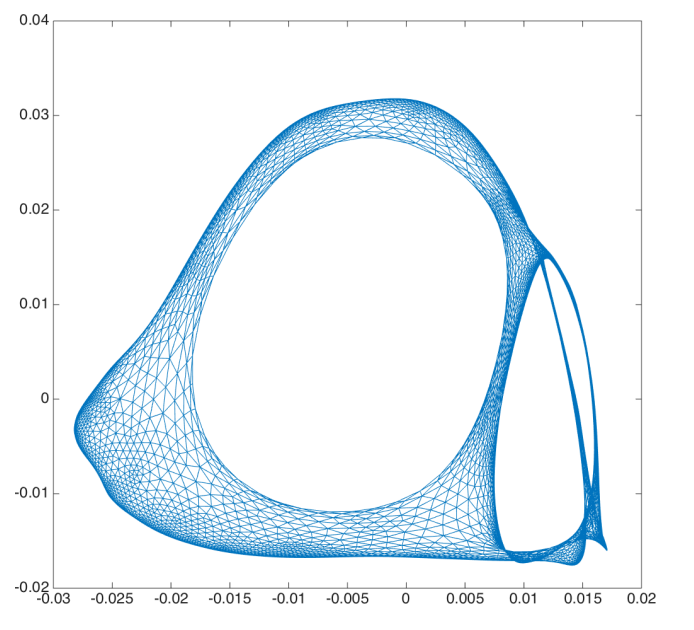
\includegraphics[trim=0cm 0cm 0cm 0cm, clip, width=10cm]{img1.png}
    \caption{First plot with (w,xy).}
    \label{fig:img2}
\end{figure}
\begin{figure}[H]
    \centering
    % Trim 5cm from each side and clip the image
    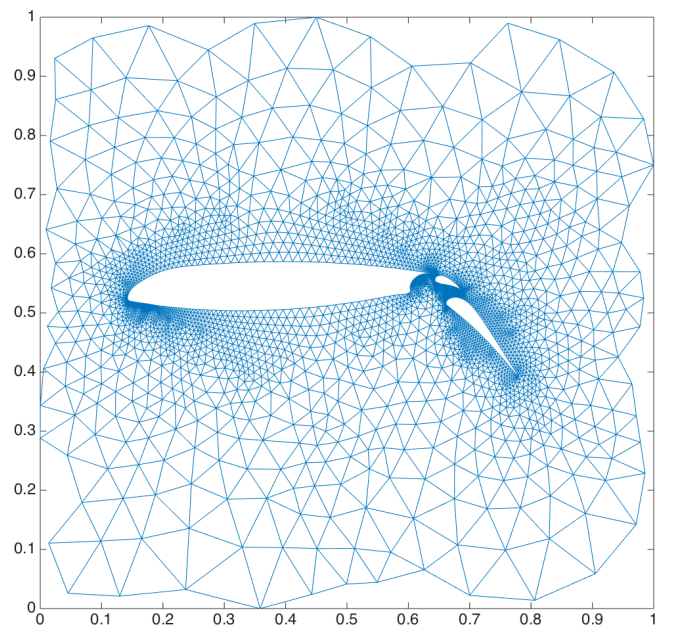
\includegraphics[trim=0cm 0cm 0cm 0cm, clip, width=10cm]{img2.png}
    \caption{Second Plot with (W, V(:, [2,3]))}
    \label{fig:img2}
\end{figure}

\subsection{k-way Spectral Clustering}

\textbf{Recursive Bi-partition:}
\begin{itemize}
    \item \textit{Method:} The method involves recursively applying a bi-partitioning algorithm in a hierarchical, divisive manner to the data set. This process continues until the desired number of clusters (\( k \)) is achieved.

    \item \textit{Advantages:} The main advantage of this approach is its simplicity in terms of the algorithmic concept, making it easy to implement and understand.

    \item \textit{Disadvantages:} However, recursive bi-partitioning can be inefficient and unstable, particularly in terms of maintaining the quality of the clusters as the number of partitions increases.
\end{itemize}

\textbf{Clustering Multiple Eigenvectors:}
\begin{itemize}
    \item \textit{Method:} This approach involves constructing a reduced space from the first \( k \) eigenvectors of the graph Laplacian. The data points are then clustered in this reduced eigenvector space.

    \item \textit{Advantages:} Clustering multiple eigenvectors makes full use of the information provided by these eigenvectors. It generally has less computational complexity compared to other methods, and the clustering results are often quite satisfactory.

    \item \textit{Disadvantages:} A key challenge is determining the appropriate number of eigenvectors to use, as not all eigenvectors contribute equally to the quality of the clustering. Often, only the first few eigenvectors provide satisfactory results, making the selection process critical and not straightforward.
\end{itemize}

In summary, k-way spectral clustering offers different approaches, each with its own set of advantages and challenges. The choice between recursive bi-partitioning and clustering multiple eigenvectors depends on the specific requirements and constraints of the clustering task at hand.


\subsection{Unnormalized Spectral Clustering}

\textbf{Input:} Given a similarity matrix \( S \in \mathbb{R}^{n \times n} \) and a specified number of clusters \( k \) to construct.

\textbf{Procedure:}
\begin{enumerate}
    \item \textit{Construct a Similarity Graph:} Form a similarity graph based on the matrix \( S \). Let \( W \) be its weighted adjacency matrix.

    \item \textit{Compute the Unnormalized Laplacian:} Calculate the unnormalized Laplacian matrix \( L \) using \( L = D - W \), where \( D \) is the degree matrix of the graph.

    \item \textit{Eigenvector Computation:} Compute the first \( k \) eigenvectors \( u_1, \ldots, u_k \) of the Laplacian matrix \( L \).

    \item \textit{Form Matrix \( U \):} Construct matrix \( U \in \mathbb{R}^{n \times k} \) which contains the vectors \( u_1, \ldots, u_k \) as columns. This step represents a dimensionality reduction from \( n \times n \) to \( n \times k \).

    \item \textit{Row Vector Formation:} For each \( i = 1, \ldots, n \), define \( y_i \in \mathbb{R}^k \) as the vector corresponding to the \( i \)-th row of \( U \).

    \item \textit{Clustering:} Apply the k-means algorithm to cluster the points \( (y_i)_{i=1, \ldots, n} \) in \( \mathbb{R}^k \) into \( k \) clusters \( C_1, \ldots, C_k \).
\end{enumerate}

\textbf{Outcome:}
This process results in the partitioning of the data into \( k \) clusters based on the spectral properties of the Laplacian matrix. The unnormalized spectral clustering approach is particularly effective in identifying underlying structures in data that are not immediately apparent in the original space.

\subsection{K-means Clustering}
K-means is one of the most well-known and widely used clustering algorithms. It clusters \( n \) objects based on attributes into \( k \) partitions, where \( k < n \), effectively grouping the objects based on attributes/features into \( k \) distinct groups.

\textbf{Algorithm Process:}
\begin{enumerate}
    \item \textit{Initialization:} Start with some initial cluster centers.
    \item \textit{Iteration:}
    \begin{itemize}
        \item Assign each example to the closest center.
        \item Recalculate the centers as the mean of the points in a cluster.
    \end{itemize}
\end{enumerate}

\textbf{Drawbacks of K-means:}

\textit{1. Euclidean Distance:}
The use of Euclidean distance treats the data space as isotropic, meaning distances remain unchanged by translation or rotation. Data points in each cluster are modeled as lying within a sphere around the cluster centroid. However, this spherical assumption may not always hold, leading to non-intuitive behaviors in clearly identifiable clusters.

\begin{figure}[H]
    \centering
    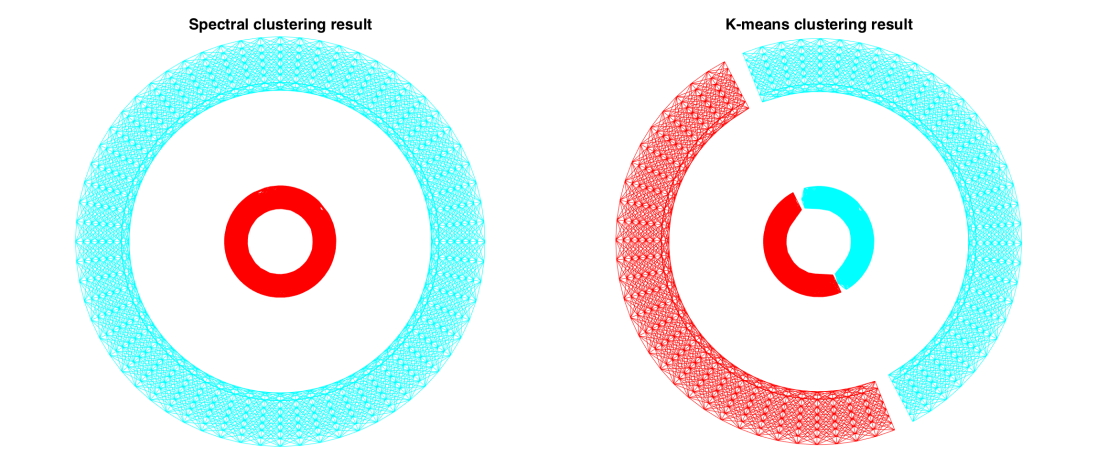
\includegraphics[trim=0cm 0cm 0cm 0cm, clip, width=10cm]{img3.png}
    \caption{K-means clustering with non-intuitive behavior.}
    \label{fig:img3}
\end{figure}

\textit{2. Impact of Outliers:}
In a linear Euclidean space, small changes in data result in proportionally small changes to the position of cluster centroids. This can be problematic when outliers are present, as they can disproportionately influence the centroid location.

\begin{figure}[H]
    \centering
    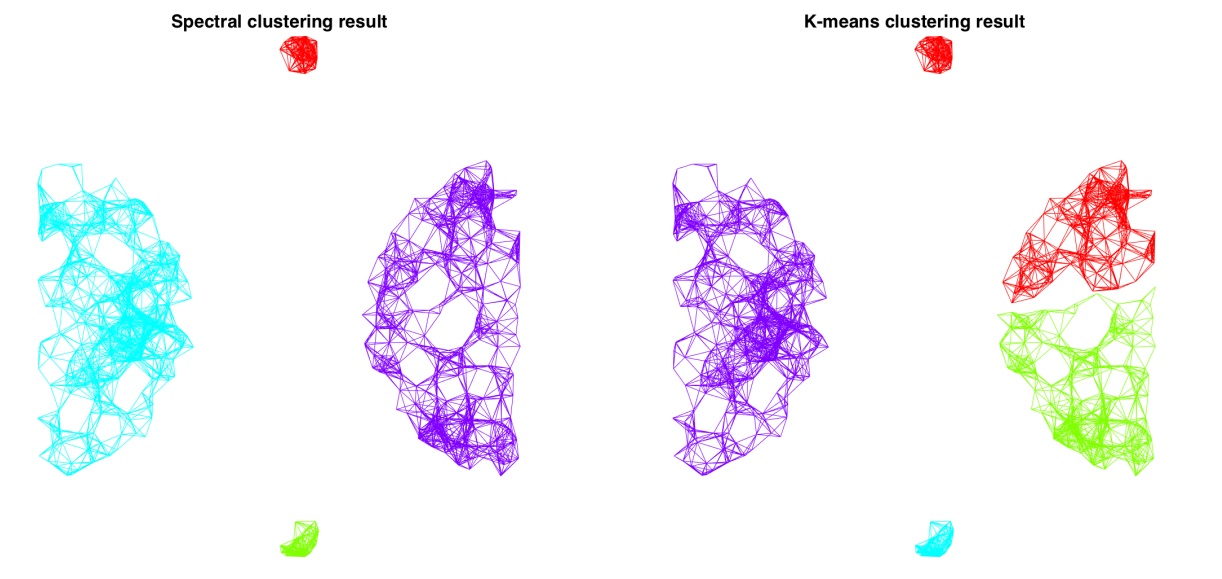
\includegraphics[trim=0cm 0cm 0cm 0cm, clip, width=10cm]{img4.png}
    \caption{Behavior of K-means in the presence of outliers.}
    \label{fig:img4}
\end{figure}

\textit{3. Equal Volume Assumption:}
K-means clusters data points based on their geometric closeness to the cluster centroid and does not account for the varying densities of each cluster. This implicit assumption that each cluster occupies the same volume in data space often leads to clusters containing an equal number of data points, which may not always be ideal.

\begin{figure}[H]
    \centering
    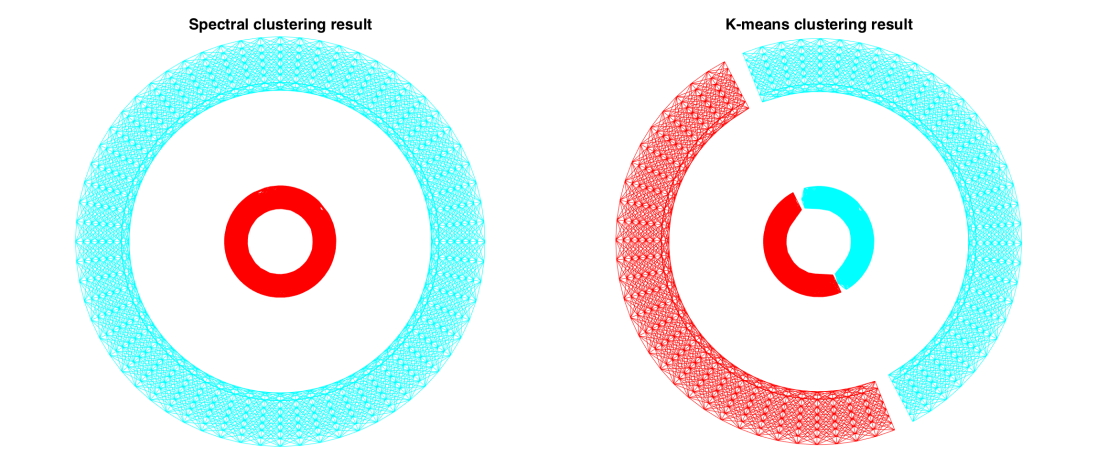
\includegraphics[trim=0cm 0cm 0cm 0cm, clip, width=10cm]{img3.png}
    \caption{K-means clustering with the same quantity of points per cluster.}
    \label{fig:img5}
\end{figure}

Despite these drawbacks, K-means remains a popular choice for clustering due to its simplicity and efficiency, particularly in scenarios where its underlying assumptions align well with the data distribution.


\subsection{Balanced Graph Partitioning Analogy}

The key insight in balanced graph partitioning is to separate points into different groups based on their similarities. The analogy involves partitioning a graph such that the edges between different groups have low weight, and edges within a group have high weight.

For a given number \( k \) of subsets, our goal is to find a partition \( A_1, \ldots, A_k \) that minimizes:
\[
\text{cut}(A_1, \ldots, A_k) = \frac{1}{2}\sum_{i=1}^{k} W(A_i, \bar{A}_i) \quad \text{(Not balanced)}
\]
\[
\text{RatioCut}(A_1, \ldots, A_k) = \sum_{i=1}^{k} \frac{\text{cut}(A_1, \ldots, A_k)}{|A_i|} \quad \text{(Balanced)}
\]

The minimum of \(\sum_{i=1}^{k}(\frac{1}{|A_i|})\) coincides.

\textbf{Example of RatioCut:}
Let \( k = 2 \). Our goal is to solve the minimization problem:
\[
\min \text{RatioCut}(A, \bar{A})
\]
Given a subset \( A \subset V \), we define the vector \( x = (x_1, \ldots, x_n)^T \in \mathbb{R}^n \) with
\[
x_i = \begin{cases}
    \sqrt{\frac{|\bar{A}|}{|A|}}, & \text{if } v_i \in A, \\
    -\sqrt{\frac{|A|}{|\bar{A}|}}, & \text{if } v_i \in \bar{A}.
\end{cases}
\]
The RatioCut objective function can be rewritten using the graph Laplacian:
\[
x^T L x = x^T D x - x^T W x = \sum_{i=1}^{n} d_i x^2_i - \sum_{i,j=1}^{n} x_i x_j w_{ij} = \ldots = \text{Rcut}(A,\bar{A}) \cdot |V|
\]
Additionally, the vector \( x \) is orthogonal to the constant vector \( \mathbf{1} \):
\[
x^T \mathbf{1} = \sum_{i=1}^{n} x_i = |A| \sqrt{\frac{|\bar{A}|}{|A|}} - |\bar{A}| \sqrt{\frac{|A|}{|\bar{A}|}} = 0
\]
And \( x \) measures the cardinality of the entire set:
\[
\|x\|^2 = x^T x = \sum_{i=1}^{n} x^2_i = |A| + |\bar{A}| = n = |V|
\]
The minimization problem
\[
\min \text{RatioCut}(A, \bar{A})
\]
can equivalently be stated as
\[
\min x^T L x \quad \text{subject to } x \perp \mathbf{1}, \|x\|^2 = n
\]

The Rayleigh-Ritz theorem indicates that the solution of this problem is given by the Fiedler eigenvector (the eigenvector corresponding to the second smallest eigenvalue of \( L \)). However, to obtain a partition of the graph, we need to convert the real-valued solution vector \( x \) of the relaxed problem into a discrete indicator vector. In spectral partitioning, we use the sign of \( x \) as an indicator function:
\[
v_i \in \begin{cases}
    A, & \text{if } x_i \geq 0, \\
    \bar{A}, & \text{if } x_i < 0.
\end{cases}
\]

Spectral clustering algorithms instead regard the coordinates \( x_i \) as points in \( \mathbb{R} \) and cluster them into two groups \( C \) and \( \bar{C} \) using a flat clustering algorithm (k-means, in this case). The clustering results are then associated with the underlying data points:
\[
v_i \in \begin{cases}
    A, & \text{if } x_i \in C, \\
    \bar{A}, & \text{if } x_i \in \bar{C}.
\end{cases}
\]

This procedure is referred to as unnormalized spectral clustering for \( k = 2 \) clusters.


\subsubsection{Computational Complexity}

The overall computational complexity of the spectral clustering algorithm is determined by the complexity of its individual components, which include the computation of eigenvalues and eigenvectors, construction of the similarity matrix, and the K-means clustering step.

\begin{itemize}
    \item \textbf{Eigenvalue and Eigenvector Computation:} The computational complexity of calculating eigenvalues and eigenvectors of a matrix is \( O(n^3) \), where \( n \) is the number of nodes in the graph. This step is often the most computationally intensive part of the process.

    \item \textbf{Similarity Matrix Construction:} Constructing the similarity matrix has a computational complexity of \( O(n^2) \). This involves calculating the pairwise similarities between all nodes, which scales quadratically with the number of nodes.

    \item \textbf{K-means Clustering:} The K-means step in spectral clustering has a complexity of \( O(nldk) \), where \( l \) is the number of iterations in the K-means algorithm, \( d \) is the dimensionality of the input data, and \( k \) is the number of clusters to be formed. The complexity depends on both the size of the dataset and the dimensions of the feature space.
\end{itemize}

Understanding these complexities is crucial in evaluating the feasibility and efficiency of spectral clustering, particularly for large-scale datasets. Optimizations and approximations may be necessary in practice to handle large \( n \), high \( d \), or when a large \( k \) is desired.

\subsection{More on Clusters}

Clustering, particularly in the context of graph theory, can be effectively formulated as a graph cut problem. This approach is especially beneficial in scenarios involving non-convex clustering, where traditional clustering methods might struggle.

\begin{itemize}
    \item \textbf{Graph Cut Formulation:} In this formulation, the objective is to partition a graph in such a way that the cut between different clusters (subgraphs) is minimized. This involves finding a balance between minimizing the edges between different clusters while maximizing the connectivity within each cluster.

    \item \textbf{Eigenvalue Decomposition of the Laplacian Matrix:} A key step in solving the graph cut problem is the eigendecomposition of the Laplacian matrix associated with the graph. This decomposition provides a representation of the data in a lower-dimensional space, which is more amenable to clustering.

    \item \textbf{Lower-Dimensional Representation:} By representing the data in a reduced dimensionality, it becomes easier to identify clusters, as the intrinsic structure of the data is more apparent in this space. This approach leverages the spectral properties of the Laplacian matrix to reveal the underlying clustering structure.

    \item \textbf{Empirical Success:} Empirically, this method of clustering has been highly successful, particularly in complex datasets where traditional clustering methods may fail to capture the true data structure. It is especially adept at uncovering the intrinsic grouping in data that is not linearly separable.
\end{itemize}

Overall, clustering as a graph cut problem, solved via eigendecomposition of the Laplacian matrix, offers a powerful and flexible approach for identifying clusters in a wide range of data types and structures.

\subsection{Project 3}

The epsilonSimGraph.mat for generate the similairty matrix of the epsilon-similairty graph.
\begin{lstlisting}
function [G] = epsilonSimGraph(epsilon,Pts)
% Construct an epsilon similarity graph
% Input
% epsilon: size of neighborhood (calculate from Prim's Algorithm)
% Pts    : coordinate list of the sample
%
% Output
% A      : the epsilon similarity matrix
S = similarityfunc(Pts, epsilon);
threshold = 0.5;
G = S >= threshold;
end
\end{lstlisting}

CreateLapl.m for create Laplacian Matrix:
\begin{lstlisting}
 function [L,Diag] = CreateLapl(W)
% Create the Laplacian matrix of a graph
% Input
% W    : Adjacency matrix
% Output
% L    : Laplacian
% Degree matrix
Diag = zeros(size(W,1));
for i = 1:size(W,1)
   Diag(i,i) = sum(W(:,i));
end
% Construct the Laplacian
L = Diag - W;
end
\end{lstlisting}

Create the gaussin similarity function
\begin{lstlisting}
 function [S] = GausSimilarityfunc(Pts, sigma)
% Create the similarity matrix S from the coordinate list of the input points
if nargin < 2
    n = length(Pts(:,1));
    sigma = log(n);
end

S = squareform(pdist(Pts));
S = exp(-S.^2 ./ (2*sigma^2));
end
\end{lstlisting}

Function to perform k-means clustering:
\begin{lstlisting}
 function [D,x] = kmeans_mod(Y,K,n)
% Function to perform k-means clustering
% --------------------------------------
% Input
% Y: data matrix
% K: # of clusters
% n: number of points
% Output
% D: centroids
% x: assignment(indicator) vector


cand = unique(round(10000*Y)/10000,'rows');
c = datasample(cand,K,'Replace',false); % pick K random input pts as initial centroids
D = c;
x = zeros(size(Y,1),1);
D_old = inf*ones(size(D));
count = 1;
while norm(D - D_old) > 0.00001 & count < 500
    D_old = D;
    % Assign points to clusters
    for i = 1:n
        min = inf;
        for k = 1:K
            dist = norm(Y(i,:) - D(k,:));
            if dist < min
                min = dist;
                x(i) = k;
            end
        end
    end

    % Update centroid locations
    for k = 1:K
        ind = find(x == k);
        if length(ind) == 1
            D(k,:) = Y(ind,:);
        else
            D(k,:) = mean(Y(ind,:));
        end
    end

    count = count + 1;
end

for i = 1:n
    min = inf;
    for k = 1:K
        dist = norm(Y(i,:) - D(k,:));
        if dist < min
            min = dist;
            x(i) = k;
        end
    end
end
end

\end{lstlisting}

KNN simalrity graph function:
\begin{lstlisting}
 function [G] = kNNSimGraph(Pts)
% Construct a k-nearest neighbors similarity graph
% Input
% k      : # of neighbors
% Pts    : coordinate list of the sample
%
% Output
% G      : the kNN similarity matrix


n = length(Pts(:,1));
kn = ceil(2*log(n));


fprintf('kNN similarity graph\n');
    for i = 1:n
        s = repmat(Pts(i,:),n,1);
        d = Pts - s;
        e = sum(d.^2,2);
        [~,ind] = sort(e);
        ind(1) = [];
        nbrs = ind(1:kn);
        G(i,nbrs) = 1;
        G(nbrs,i) = 1;
    end
end
\end{lstlisting}
\section{Image Deblurring and Conjugate Gradient Solver}

We explore solving a system of linear equations \( Ax = b \), where \( A \in \mathbb{R}^{n \times n} \) is a nonsingular coefficient matrix, \( b \in \mathbb{R}^n \) is a constant vector, and \( x \in \mathbb{R}^n \) is the unknown solution vector.

\subsection{Direct Methods}
Direct methods are designed to compute the exact solution in a finite number of steps. Their characteristics include:
\begin{itemize}
    \item \textbf{Computational Cost:} The cost for classical Gaussian elimination is \( O(n^3) \). For sparse matrices, this cost reduces to \( O(n^{1.5}) \) or \( O(n^2) \).

    \item \textbf{Memory Consumption:} These methods have a high memory requirement due to additional fill-in elements created during the elimination process.

    \item \textbf{Limitation:} The complexity of Gaussian elimination becomes prohibitively high for large systems of linear equations.
\end{itemize}

This complexity leads to the consideration of alternative approaches, particularly iterative methods.

\subsection{Iterative Methods}
Iterative methods start with an arbitrary initial guess and iteratively compute an approximate solution:
\begin{itemize}
    \item \textbf{Computational Cost:} The cost for the conjugate gradient algorithm ranges between \( O(n) \) and \( O(n^{3/2}) \), making it more scalable for large systems.

    \item \textbf{Memory Efficiency:} These methods do not require additional memory for fill-ins, which is beneficial for large systems.

    \item \textbf{Convergence:} The convergence of iterative methods depends on the properties of matrix \( A \) and typically occurs after a few iterations. This makes them suitable for problems where an exact solution is not necessary, or where the exact solution is computationally infeasible.
\end{itemize}

In summary, while direct methods offer exact solutions, their computational and memory demands make them less viable for large systems. Iterative methods, such as the conjugate gradient algorithm, provide a practical alternative by offering approximate solutions with lower computational and memory requirements.

\subsubsection{Sketch of an Iterative Method}

The algorithm for an iterative method can be structured as follows:

\begin{enumerate}
    \item \textbf{Initialization:} Start with \( m = 0 \) and set \( x^m \) as the initial guess for the solution.

    \item \textbf{Iteration:} Repeat the following steps until the error estimate is less than a predetermined threshold \( \epsilon \):
    \begin{enumerate}
        \item Compute a new solution \( x^{m+1} \).
        \item Update the error estimate based on \( x^{m+1} \).
    \end{enumerate}
\end{enumerate}

\subsubsection{Definition of Error and Residual}

In iterative methods, two important concepts are \textit{Error} and \textit{Residual}, which help in measuring the accuracy of the solution at each iteration.

\begin{itemize}
    \item \textbf{Error:} The error at step \( m \) quantifies the deviation of the approximate solution \( x^(m) \) from the exact solution \( x \). It is defined as:
    \[
    e^(m) = x - x^(m) = A^{-1}b - x^(m)
    \]
    Here, \( e^(m )\) represents the difference between the true solution and the current approximation.

    \item \textbf{Residual:} The residual is a measure of the real error and is relatively easier to compute compared to the error. It is defined as:
    \[
    r^(m) = b - Ax^(m) = Ae^(m)
    \]
    This expression shows that the residual \( r^(m) \) is equivalent to the error transformed by the matrix \( A \) (i.e., \( Ae^(m) \)). The significance of this relationship will be evident in subsequent discussions.

    \item \textbf{Residual Norm:} The norm of the residual, denoted as \( ||r^(m)|| \), quantifies the magnitude of the residual. Additionally, the relative residual norm is defined as \( \frac{||r^(m)||}{||b||} \), which normalizes the residual norm by the norm of the constant vector \( b \) in the system \( Ax = b \).
\end{itemize}

Understanding error and residual, and their respective norms, is crucial in assessing the convergence and accuracy of iterative methods in solving systems of linear equations.
\newline
$x^(m)$ is the approximation in the m-th iteration.

\subsection{Minimization Problem in 1D Case}

The basic idea in this context is to transform the linear equation \( a \cdot x = b \) into an equivalent minimization problem. This approach involves defining a function \( f(x) \) whose minimum we seek to find.

\begin{itemize}
    \item \textbf{Minimization Function:} The function to be minimized is given by:
    \[
    f(x) := \frac{1}{2}a \cdot x^2 - b \cdot x \quad (1)
    \]
    where \( a \) is a scalar coefficient and \( b \) is a constant term.

    \item \textbf{Precondition:} We assume that \( a \) is symmetric and positive definite. In the context of a scalar coefficient, this simply means \( a > 0 \)
    \[
    f'(x) = 2 \cdot \frac{1}{2} x-b = ax-b
    \]

    \item \textbf{Solving the Minimization Problem:} Setting the derivative equal to zero, \( f'(x) = 0 \), leads us back to the original problem:
    \[
    a \cdot x = b
    \]
    This shows that solving the minimization problem \( f(x) \) is equivalent to solving the linear equation \( a \cdot x = b \), under the precondition that \( a \) is positive.
\end{itemize}

\subsubsection{Minimization Problem}
\begin{itemize}
 \item {\textbf{Basic Idea}\newline
 Instead of Ax =b solve an equivalent minimization problem \[f(x) := \frac{1}{2}\langle Ax,x \rangle -\langle b,x\rangle\]
 \item{\textbf{Precondition}, let A be a symmetric positive definite matrix: \newline
 \[
  \langle Ax,x\rangle >0, if x \neq zero vector
 \]
 if we take the derivative of (3) it will lead to: \[
                                                    f'(x) = \frac{1}{2}A^Tx+\frac{1}{2} Ax-b = Ax-b \quad condition: A^t=A\]
}
}
\end{itemize}

\begin{itemize}
 \item Linear equations with solution at the interesection of both lines.
 \item Quadratic From $f(x)$ and gradients $f'(x)$
\end{itemize}

\subsubsection{Method of Steepest Descent}

The method of steepest descent is an iterative approach used for finding the minimum of a function. It involves taking steps proportional to the negative of the gradient of the function at the current point.

\begin{itemize}
    \item \textbf{Basic Idea:} At each iteration, take a step in the direction of the negative gradient at the current point \( x^{(m)} \). This direction is given by \( -f'(x^{(m)}) \).

    \item \textbf{Step Length:} Choose a step length such that the function \( f \) is minimized along this search direction.
\end{itemize}

\textbf{Algorithm:}
\begin{enumerate}
    \item Initialize the residual: \( r^{(0)} = b - Ax^{(0)} \).

    \item Repeat until the norm of the residual \( ||r^{(0)}|| \) is less than a threshold \( \epsilon \):
    \begin{enumerate}
        \item Find a scalar \( \alpha \) that minimizes \( f(x^{(m)} + \alpha r^{(m)}) \).

        \item Update the solution: \( x^{(m+1)} = x^{(m)} + \alpha r^{(m)} \).

        \item Update the residual: \( r^{(m+1)} = b - Ax^{(m+1)} \).
    \end{enumerate}
\end{enumerate}

In this method, the residual not only measures the error but also serves as the search direction for the next iteration.
\newline \newline
The goal is to minimize the function \( f \) along a chosen search vector \( p^{(m)} \).
\newline
\textbf{Approach:}
To find the minimum of \( f \) along \( p^{(m)} \), we consider the function at the point \( x^{(m+1)} = x^{(m)} + \alpha p^{(m)} \). The condition for \( f \) to be minimized at this point is given by setting its derivative with respect to \( \alpha \) to zero:
\[
\frac{d}{d\alpha} f(x^{(m+1)}) = 0
\]

\textbf{Using the Chain Rule:}
By applying the chain rule, we can express this derivative as:
\[
\frac{d}{d\alpha} f(x^{(m+1)}) = \left\langle f'(x^{(m+1)}), \frac{d}{d\alpha}(x^{(m)} + \alpha p^{(m)}) \right\rangle
\]
where \( \langle \cdot, \cdot \rangle \) denotes the inner product. Simplifying further, we get:
\[
\frac{d}{d\alpha} f(x^{(m+1)}) = \langle r^{(m+1)}, p^{(m)} \rangle
\]

\textbf{Steepest Descent Specifics:}
For the method of steepest descent, we specifically choose \( p^{(m)} = r^{(m)} \), where \( r^{(m)} \) is the residual at the \( m \)-th iteration. This choice leads to a descent direction that is steepest in terms of the current position in the function's domain.
\newline
We search for an $\alpha$, such that $r^{(m+1)} \perp p^{(m)}$ \newline
Rearraging for $\alpha$:\newline
\[
 \langle r^{(m+1)}, p^{(m)} \rangle = 0 \newline
 ... \newline
 \alpha = \frac{\langle r^{(m)}, p^{(m)} \rangle}{\langle Ap^{(m)}, p^{(m)} \rangle}
\]
\newline

The algorithm for the method of steepest descent is summarized as follows:

\begin{enumerate}
    \item \textbf{Initialization:} Start with the initial residual computed as \( r^{(0)} = b - Ax^{(0)} \).

    \item \textbf{Iterative Process:} Repeat the following steps until the norm of the residual \( ||r^{(m)}|| \) is less than a predetermined threshold \( \epsilon \):
    \begin{align*}
        \alpha^{(m)} &= \frac{\langle r^{(m)}, r^{(m)} \rangle}{\langle Ar^{(m)}, r^{(m)} \rangle} \\
        x^{(m+1)} &= x^{(m)} + \alpha^{(m)} r^{(m)} \\
        r^{(m+1)} &= r^{(m)} - \alpha^{(m)} Ar^{(m)}
    \end{align*}

    \item \textbf{Efficiency Note:} The computation of \( r^{(m+1)} \) does not require the matrix-vector product \( Ax^{(m)} \). Instead, it utilizes the expression \( r^{(m+1)} = r^{(m)} - \alpha^{(m)} Ar^{(m)} \), enhancing computational efficiency.
\end{enumerate}

This algorithm effectively implements the steepest descent method by iteratively updating the solution vector \( x^{(m)} \) and the residual \( r^{(m)} \) using the calculated step size \( \alpha^{(m)} \).
\begin{figure}[H]
    \centering
    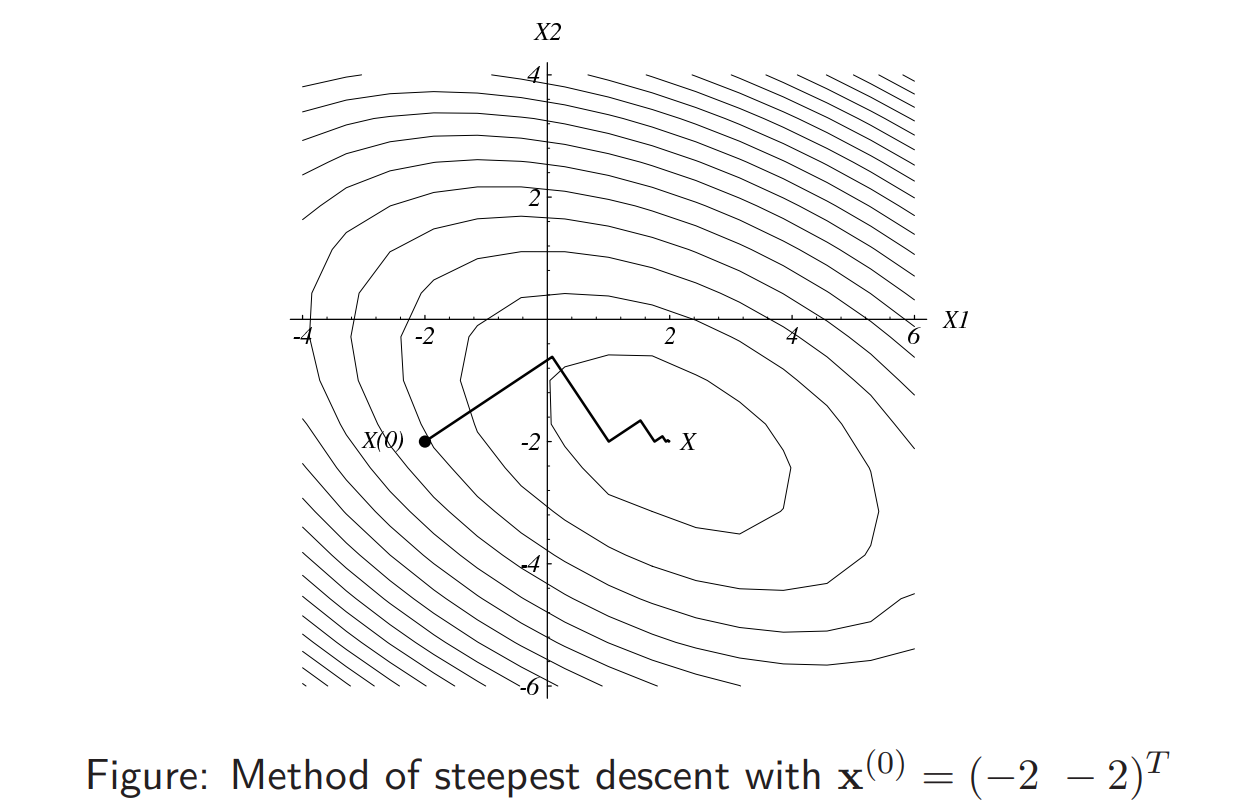
\includegraphics[trim=0cm 5cm 0cm 0cm, clip, width=10cm]{img6.png}
    \caption{Method of steeperst descent with $x^{(0)}=(-2 -2)^T$}
    \label{fig:img6}
\end{figure}
Consider the function \( f(x) = \frac{1}{2} \langle Ax, x \rangle - \langle b, x \rangle \), which we aim to minimize to compute the solution of \( Ax = b \).

\textbf{Example for \( n = 2 \):}
Suppose matrix \( A \) has two orthogonal eigenvectors \( v_1 \) and \( v_2 \) with associated eigenvalues \( \lambda_1 \) and \( \lambda_2 \). Any vector \( x \) can be expressed as a linear combination of these eigenvectors:
\[
x = a_1 \cdot v_1 + a_2 \cdot v_2, \quad a_1, a_2 \in \mathbb{R}
\]

For the case where \( b = 0 \), the function \( f(x) \) can be expanded as follows:
\begin{align*}
f(x) &= \frac{1}{2}x^T A x \\
&= \frac{1}{2}(a_1 v_1 + a_2 v_2)^T (a_1 \lambda_1 v_1 + a_2 \lambda_2 v_2) \\
&= \frac{1}{2}(a_1^2 \lambda_1 + a_2^2 \lambda_2)
\end{align*}

This expression represents the function \( f(x) \) in terms of the eigenvalues and eigenvectors of \( A \).

\begin{figure}[H]
    \centering
    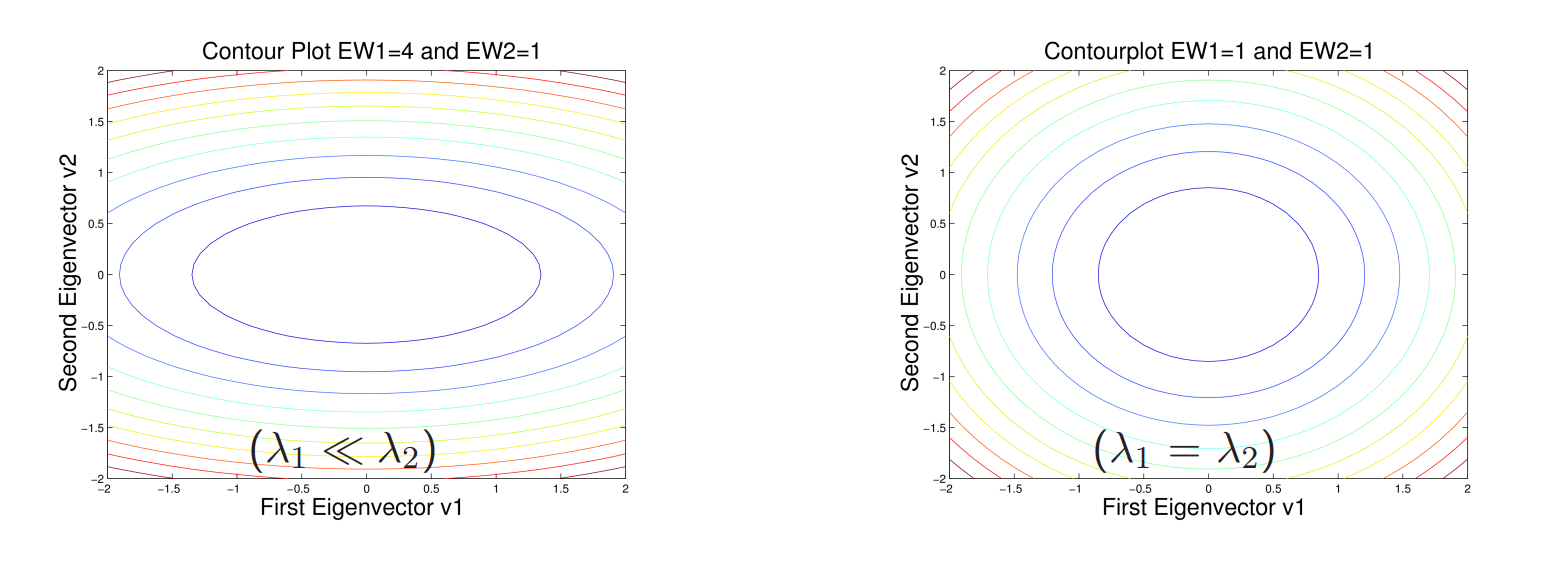
\includegraphics[trim=0cm 0cm 0cm 0cm, clip, width=15cm]{img7.png}
    \caption{Contour lines of the functional.}
    \label{fig:img7}
\end{figure}

\subsubsection{Impact on Convergence}

The condition number of a matrix significantly impacts the convergence behavior of iterative methods like steepest descent. The influence can be summarized as follows:

\begin{itemize}
    \item \textbf{Large Condition Number with Good Starting Point:}
    If the condition number of the matrix is large and the initial guess is by chance close to the true solution, the steepest descent method may converge quickly. However, this fast convergence is more accidental and not guaranteed.

    \item \textbf{Large Condition Number with Bad Starting Point:}
    Conversely, if the condition number is large and the starting point is not close to the solution, the convergence of the steepest descent method can be very slow. This scenario underscores the sensitivity of the method to initial guesses.

    \item \textbf{Small Condition Number:}
    A matrix with a small condition number generally leads to good convergence properties of the steepest descent method, regardless of the starting vector. This consistent performance is one of the reasons why preconditioning (which aims to reduce the condition number) is a valuable approach in iterative methods.
\end{itemize}
\subsection{Conjugate Gradient Method}

\textbf{Basic Idea:}
The Conjugate Gradient Method improves upon the steepest descent method by considering optimal search steps in each iteration.

\textbf{Approach:}
\begin{itemize}
    \item Define \( n \) orthogonal search directions, \( p^{(0)}, p^{(1)}, \ldots, p^{(n-1)} \), allowing for a maximum of \( n \) steps.
    \item The minimization criterion is based on the orthogonality of the error \( e^{(m+1)} \) with the search direction \( p^{(m)} \), such that \( p^{(m)} \perp e^{(m+1)} \).
\end{itemize}
\begin{figure}[H]
    \centering
    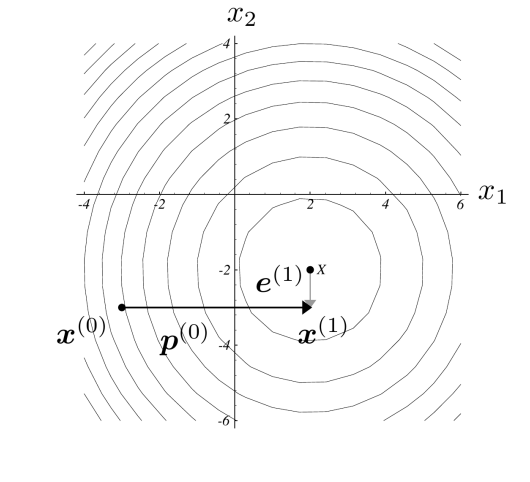
\includegraphics[trim=0cm 0cm 0cm 0cm, clip, width=10   cm]{img8.png}
    \caption{Illustration of the orthogonality in the Conjugate Gradient Method.}
    \label{fig:img8}
\end{figure}

\textbf{Error Elimination:}
Each step eliminates the error component in the current search direction. If \( p^{(m)} \perp e^{(m+1)} \), then the scalar product must be zero:
\[
\langle p^{(m)}, e^{(m+1)} \rangle = 0
\]
\[
\langle p^{(m)}, e^{(m)} + \alpha^{(m)} p^{(m)} \rangle = 0
\]
\[
\alpha^{(m)} = -\frac{\langle p^{(m)}, e^{(m)} \rangle}{\langle p^{(m)}, p^{(m)} \rangle}
\]
However, \( e^{(m)} \) is typically unknown.

\textbf{A-Orthogonality:}
To overcome this, the method uses \( A \)-orthogonal (or conjugate) vectors. Two vectors \( a \) and \( b \) are \( A \)-orthogonal if:
\[
a^T A b = \langle a, Ab \rangle = 0 \quad \Leftrightarrow \quad a \perp_A b
\]
For \( p^{(m)} \perp_A e^{(m+1)} \) and \( r^{(m)} = Ae^{(m)} \):
\[
\langle p^{(m)}, Ae^{(m+1)} \rangle = 0
\]
\[
\langle p^{(m)}, Ae^{(m)} + \alpha^{(m)} Ap^{(m)} \rangle = 0
\]
\[
\alpha^{(m)} = -\frac{\langle p^{(m)}, Ae^{(m)} \rangle}{\langle p^{(m)}, Ap^{(m)} \rangle} = \frac{\langle p^{(m)}, r^{(m)} \rangle}{\langle p^{(m)}, Ap^{(m)} \rangle}
\]


\begin{figure}[H]
    \centering
    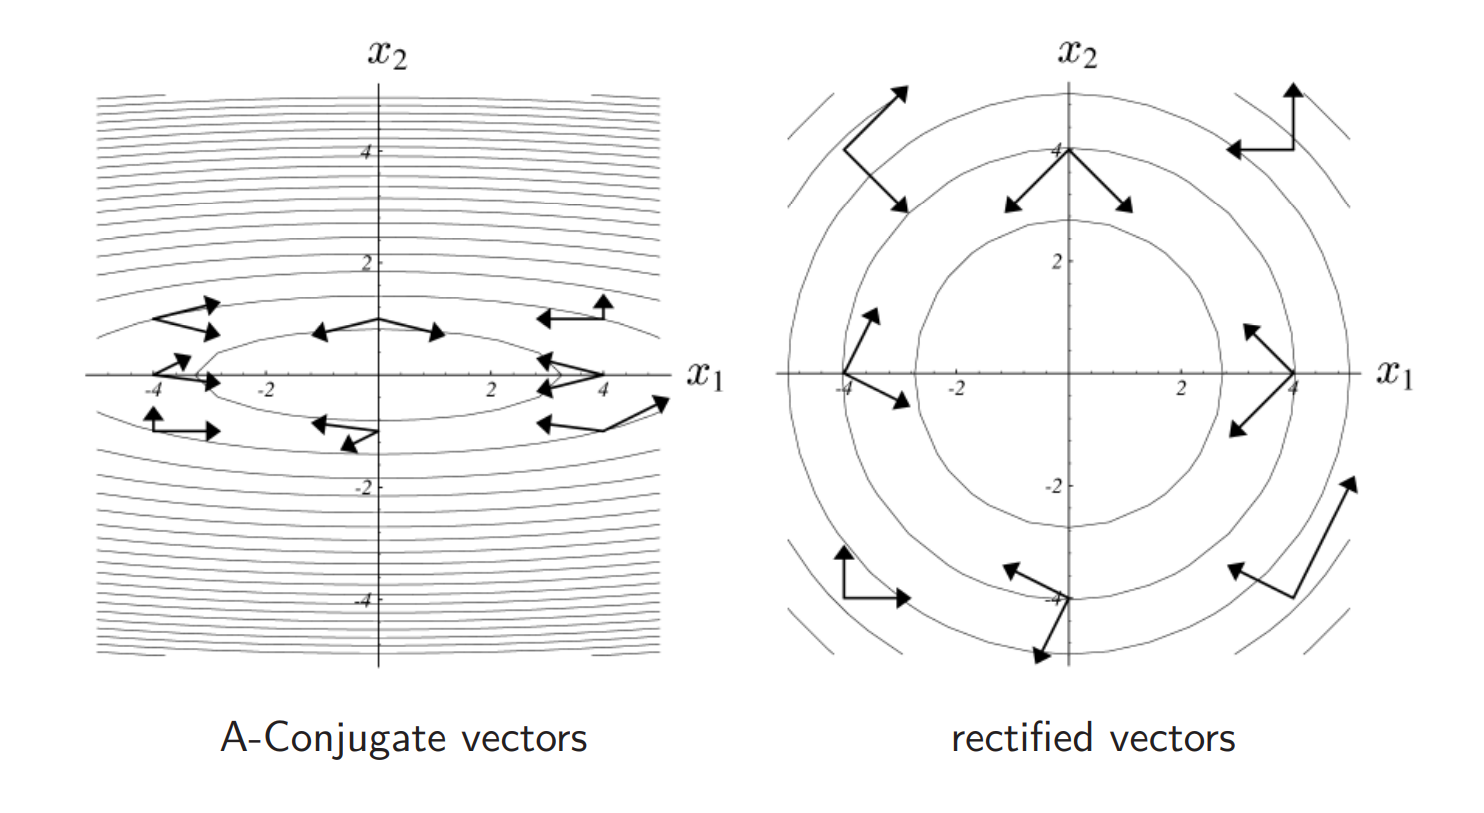
\includegraphics[trim=0cm 0cm 0cm 0cm, clip, width=15cm]{img9.png}
    \caption{Further demonstration of \( A \)-orthogonality in the method.}
    \label{fig:img9}
\end{figure}

\subsection{Conjugate Directions}

\textbf{Conditions:}
For the minimization of \( f'(x^{(m)} + \alpha p^{(m)}) \), the algorithm iteratively follows these steps:

\begin{enumerate}
    \item \textbf{Initialization:} Start with \( r^{(0)} = b - Ax^{(0)} \).

    \item \textbf{Iterative Process:} For all \( m = 1, \ldots, n \):
    \begin{itemize}
        \item Select a search vector \( p^{(m)} \) that is conjugate to all previously computed \( p^{(l)} \) for \( l < m \).
        \item Compute \( \alpha^{(m)} \) and update \( x^{(m+1)} \) and \( r^{(m+1)} \) as:
        \begin{align*}
            \alpha^{(m)} &= \frac{\langle r^{(m)}, p^{(m)} \rangle}{\langle Ap^{(m)}, p^{(m)} \rangle} \\
            x^{(m+1)} &= x^{(m)} + \alpha^{(m)} p^{(m)} \\
            r^{(m+1)} &= r^{(m)} - \alpha^{(m)} Ap^{(m)}
        \end{align*}
    \end{itemize}
\end{enumerate}
\subsubsection{Conjugate Gradient Method}

\textbf{Basic Idea:}
The Conjugate Gradient Method iteratively constructs conjugate search directions using residuals.

\textbf{Search Direction:}
\begin{itemize}
    \item Construct the next search direction \( p^{(m+1)} \) using the residual \( r^{(m+1)} \) and a scaling factor \( \beta^{(m+1)} \):
    \[ p^{(m+1)} = r^{(m+1)} + \beta^{(m+1)} p^{(m)} \]
    \item The factor \( \beta^{(m+1)} \) is chosen to ensure \( A \)-orthogonality:
    \[ \beta^{(m+1)} = -\frac{\langle r^{(m+1)}, Ap^{(m)} \rangle}{\langle p^{(m)}, Ap^{(m)} \rangle} = \frac{\langle r^{(m+1)}, r^{(m+1)} \rangle}{\langle r^{(m)}, r^{(m)} \rangle} \]
    \item The initial search vector is \( r^{(0)} \).
\end{itemize}

\textbf{Krylov-Subspace:}
The method constructs a Krylov-subspace \( U_m \) defined as:
\[ U_m := \text{span}\{p^{(0)}, Ap^{(0)}, A^2p^{(0)}, \ldots, A^mp^{(0)}\} \]

\textbf{Algorithm Steps:}
\begin{enumerate}
    \item \textbf{Initialization:} Start with \( r^{(0)} := b - Ax^{(0)} \), where \( x^{(0)} \) is arbitrary, and set \( p^{(0)} := r^{(0)} \).
    \item \textbf{Iteration:} For \( m = 0, 1, \ldots, n-1 \):
    \begin{itemize}
        \item Calculate step length \( \alpha^{(m)} \) and update solution \( x^{(m+1)} \) and residual \( r^{(m+1)} \):
        \[ \alpha^{(m)} = \frac{\langle r^{(m)}, p^{(m)} \rangle}{\langle Ap^{(m)}, p^{(m)} \rangle} \]
        \[ x^{(m+1)} = x^{(m)} + \alpha^{(m)} p^{(m)} \]
        \[ r^{(m+1)} = r^{(m)} - \alpha^{(m)} Ap^{(m)} \]
        \item Compute \( \beta^{(m+1)} \) and update search direction \( p^{(m+1)} \):
        \[ \beta^{(m+1)} = \frac{\langle r^{(m+1)}, r^{(m+1)} \rangle}{\langle r^{(m)}, r^{(m)} \rangle} \]
        \[ p^{(m+1)} = r^{(m+1)} + \beta^{(m+1)} p^{(m)} \]
    \end{itemize}
\end{enumerate}

\textbf{Elements of the Algorithm:}
\begin{itemize}
    \item \( x^{(m)} \): Approximate solution at step \( m \).
    \item \( r^{(m)} \): Residual at step \( m \).
    \item \( p^{(m)} \): Search direction at step \( m \).
    \item \( \alpha^{(m)} \): Step length in search direction \( p^{(m)} \) for next iterate \( x^{(m+1)} \).
    \item \( \beta^{(m+1)} \): Factor to compute new search direction \( p^{(m+1)} \) from \( r^{(m+1)} \) and \( p^{(m)} \), ensuring \( A \)-orthogonality.
\end{itemize}

The exact solution is theoretically obtained after \( n \) iterations, making the Conjugate Gradient method a direct method. However, in practice, fewer iterations are often sufficient for an approximate solution.

\subsection{Preconditioning in Conjugate Gradient Method}

\textbf{Problem:}
The rate of convergence of the Conjugate Gradient (CG) method is heavily influenced by the condition number of matrix \( A \), denoted as \( k(A) \). The convergence relation is given by:
\[
||x^{(m)} - x^*||_A \leq 2 \left( \frac{\sqrt{k(A)} - 1}{\sqrt{k(A)} + 1} \right)^m ||x_0 - x^*||_A
\]
where the condition number \( k(A) \) is defined as:
\[
k(A) = ||A||_2 ||A^{-1}||_2 = \frac{\lambda_{\text{max}}(A)}{\lambda_{\text{min}}(A)}
\]
If \( k(A) \) is significantly greater than 1, the convergence rate is slow.

\textbf{Basic Idea of Preconditioning:}
To improve the condition number of \( A \) by applying a preconditioner \( M \), such that \( k(M^{-1}A) \) is much smaller than \( k(A) \). The equivalent problem becomes \( M^{-1}Ax = M^{-1}b \), where:
\begin{itemize}
    \item \( M \) should be easy to invert.
    \item The resulting matrix \( M^{-1}A \) must remain symmetric positive definite (SPD) for the CG method to be applicable.
    \item Decompose \( M \) as \( EE^T = M \) to transform \( Ax = b \) into \( E^{-1}AE^{-T}\hat{x} = E^{-1}b \), where \( \hat{x} = E^Tx \) and \( E^{-1}AE^{-T} \) is SPD.
\end{itemize}

\textbf{Methods of Preconditioning:}
\begin{enumerate}
    \item \textbf{Diagonal Preconditioning:} Choose \( M = \text{diag}(A) \).
    \item \textbf{Incomplete LU-decomposition:} Choose \( M = LU \approx A - R \), where it is crucial that the fill-in and the time for factorization are minimized.
\end{enumerate}

Effective preconditioning enhances the performance of the CG method by reducing the condition number, thereby accelerating the convergence rate.


% %
%
% \subsubsection{Jacobi Iteration Method}
% Basic Idea: solve the equation for every component $x_j$ using the current approximation of x:
% - FOr each individual elements of x we will use the following iterations method:
% \[
%  x_j^{(m+1)} = \frac{1}{a_{jj}}(_j-\sum_{k\neq a_{jk}x_k^(m))
% \]
% we will only use elements from the previous iteration. THe order in which the equations are examined is irreelevant since the jacobi method treats them independetly. \newline
% Matrix formulation: split A in: \newline
% $$A = D+E$$
% where D are all diagonal elements of A and E are the off-diagonal elements of A.
% \[
%  Ax = b \newline
%  Dx = -Ex+b \newline
%  x = -D^{-1}Ex+D^{-1}b \newline
%  x = R_{jk}+c_j \newline
%  x^{m+1} = R_jx^{(m)}+c_j
% \]
% The fundametal convergence results can be proven by using an eigenvalue anyles of R.
% We need to remeber the following Definitions:\newline
% - The spectral Radius of matrix A is:
% \[
%  p(A) = max{|\lambda|:\lambda eigenvalue of A}
% \]
% The spectral condition number is given by \[
%                                            k = \lambda_{max}/ \lambda_{min}
%                                           \]
% Let A a symmetric, real $nxn$ matrix. The vector x is called an eigenvector to the scalr eigevalue $\lambda$ if the following eqaution is satisfied: \newline
% $$Ax =\lambda x$$
% geometric interpretation of the matrix-vector multiplication: the multiplication of a matrix A with a vector x is linear operator, which consisits of a scaling and a rotation of a vector x \[
%                                                                                                                                                                                               A = \begin{bmatrix}
%                                                                                                                                                                                         2&1\\1&2                                                                                                                                                                                                  \end{bmatrix}
% , x = \begin{bmatrix}
%        2\\1
%       \end{bmatrix}, y=Ax= \begin{bmatrix}
%       5\\4
%       \end{bmatrix}\]
%
%       The eigenvector x to the associated eigenvalue will scaled with $\lambda$ under the transformation $Ax=\lambda x$. The matrix A has the following eigenvalues and eigenvectors $x_1 = (1 1)^T$ with eigevnalue $\lambda_1 = 3$ and $\x_2 = (1 -1)^T$ with eigenvalue $\lambda_2=1$
%
% \begin{figure}[H]
%     \centering
%     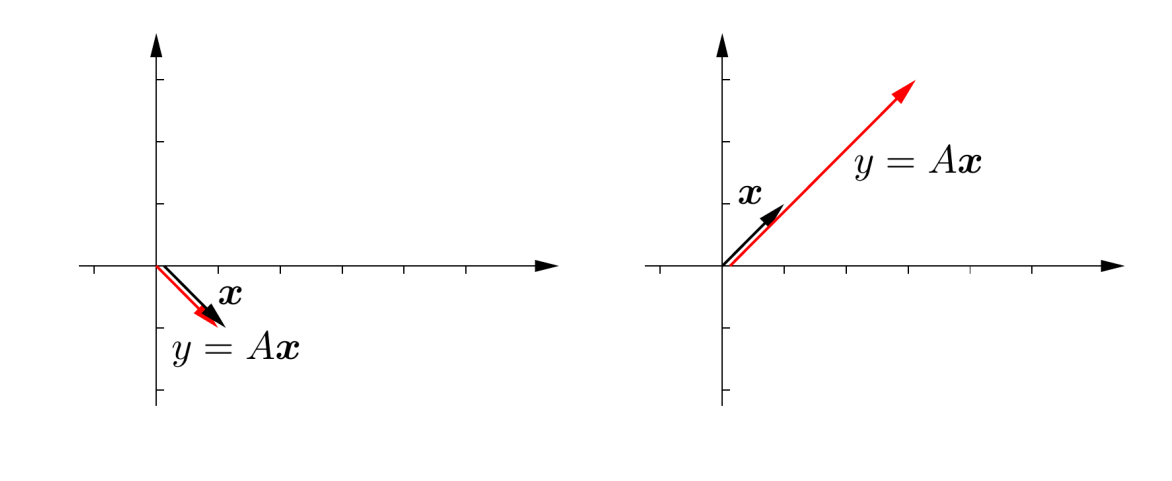
\includegraphics[trim=0cm 0cm 0cm 0cm, clip, width=15cm]{img10.png}
%     \caption{Graphical reresentation of the vectors.}
%     \label{fig:img10}
% \end{figure}
%
% Theorem: A symmetric real matrix of dimension nxn has n eigenvalues $\lambda_k$ with associated eigenvectors $x_k(k=1,..,n)$ the eigenvecotrs ${x_1, x_2,..., x_n}$ build a complete system of n orthonromal vectors: \[
%                                                                                                                                                                                                                        \langle x_i, x_j \rangle = 1 if i=j, \newline
%
%                                                                                                                                                                                                                        and \langle x_i,x_j \rangle = 0 if i\neq j
%                                                                                                                                                                                                                       \]
%



          \subsubsection{Jacobi Iteration Method}
The Jacobi Iteration Method is an iterative process for solving a system of linear equations by updating each variable independently in a systematic manner.

\textbf{Iterative Formula:}
In the Jacobi Iteration Method, each component \( x_j \) of the solution vector is updated using the current approximation of the other components:
\[
 x_j^{(m+1)} = \frac{1}{a_{jj}} \left( b_j - \sum_{k \neq j} a_{jk} x_k^{(m)} \right)
\]
This method treats each equation independently, allowing for parallel computation.

\textbf{Matrix Formulation:}
The matrix \( A \) is decomposed into its diagonal components \( D \) and off-diagonal components \( E \):
\[
 A = D + E
\]
The iterative process can then be expressed in matrix form as:
\[
 Ax = b \Rightarrow Dx = -Ex + b \Rightarrow x = -D^{-1}Ex + D^{-1}b
\]
\[
 x^{(m+1)} = R_j x^{(m)} + c_j
\]
where \( R_j = -D^{-1}E \) and \( c_j = D^{-1}b \).

\textbf{Spectral Radius and Convergence:}
The convergence of the Jacobi method is governed by the spectral radius of the matrix \( R_j \):
\[
 p(R_j) = \max \{ |\lambda| : \lambda \text{ is an eigenvalue of } R_j \}
\]
The Jacobi iteration converges if and only if the spectral radius \( p(R_j) < 1 \).

\textbf{Geometric Interpretation:}
Consider a symmetric, real \( n \times n \) matrix \( A \) with eigenvectors \( x_k \) corresponding to eigenvalues \( \lambda_k \). The multiplication of \( A \) with a vector \( x \) is a linear transformation involving scaling and rotation:
\[
 A = \begin{bmatrix}
 2 & 1 \\
 1 & 2
 \end{bmatrix}, \quad
 x = \begin{bmatrix}
 2 \\
 1
 \end{bmatrix}, \quad
 y = Ax = \begin{bmatrix}
 5 \\
 4
 \end{bmatrix}
\]
The eigenvectors of \( A \) form an orthonormal basis, and any vector can be represented as a linear combination of these eigenvectors.

\textbf{Eigenvector Representation:}
A symmetric real matrix has eigenvalues \( \lambda_k \) with associated orthonormal eigenvectors \( x_k \). These eigenvectors form a complete system of orthonormal vectors:
\[
 \langle x_i, x_j \rangle =
 \begin{cases}
 1 & \text{if } i = j, \\
 0 & \text{if } i \neq j.
 \end{cases}
\]

\begin{figure}[H]
    \centering
    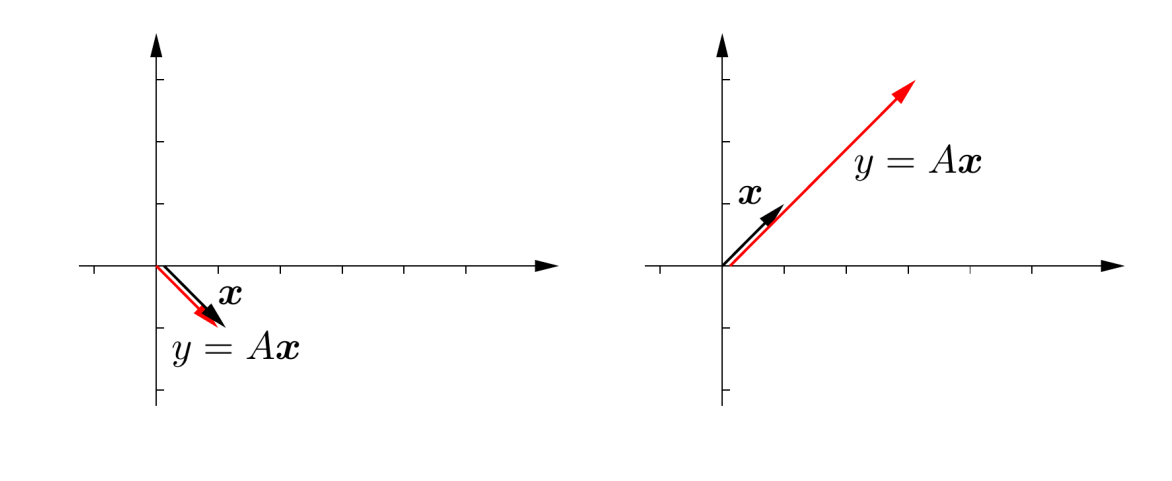
\includegraphics[trim=0cm 0cm 0cm 0cm, clip, width=15cm]{img10.png}
    \caption{Graphical representation of the Jacobi Iteration Method.}
    \label{fig:img10}
\end{figure}

\textbf{Theorem and Convergence Criteria:}
The Jacobi iteration converges for all starting vectors if the spectral radius \( p(R_j) < 1 \). Good convergence is typically observed when the matrix \( A \) is close to the identity matrix or when the spectral condition number is close to 1.

%
% \textbf{Convergence of the jacobi-iteration}
% Theorem, the iteration $x^{(m)} =R_jx^{(m+1)} +c_j$ converges for all starting vectord $x^{(0)}$ againtst a solution $x^*$ ifn and only if $p(R_j)<1$\newline
% Explainantion: every vector $\mathbb{R}^n$ can be written as a liner combination of eigenvectors from R (if R is not singular). If one eigenvaluie is larger that 1, then the jacobi-iteration will not converge. \newline
%
% general criteria for good converge:
% - k ~~ 1, small p
% - A close to the identiy matrix I
% - All these method will convergence in one iteraion of $A =\beta I$
% \newline
% Here we can see how the itearion will effect the error term $e^{(m)}$
% \[
%  x^{(m=1)} = R_jx^{(m)} +c_j\newline
%  = R_j(x+e^{(m)}+c_j \newline
%  = R_jx+c_j + R_je^{(m)} \newline
%  = x + R_je^{(m)}
%  \newline
%
%  e^{(m+1)} = R_je^{(m)} \quad |(x-x^{(m+1)} = e^{(m+1)}
%
% \]
% if p(R) < 1, then the error will converges 0 (with $m -> \infitiy$\newline
% A better but still very easy method is the gaus-seidel-iteration. In pricinple, the idea is very similar to the jacobi method, but it uses immediately new componets $x_j^{(m+1)}$ \[
%                   x_j^{(m+1)} = \frac{1}{a_{jj}}(b_j-\sum_{k=1}^{j=1}a_{jk}x_k^{m+1} - \sum_{k=j+1}^na_{jk}x_k^{(m)}
%                                                                                                                                                                                    \]

\subsubsection{Convergence of the Jacobi Iteration Method}
The convergence of the Jacobi iteration method is crucial for its effectiveness in solving linear systems. This convergence is determined by the spectral properties of the matrix involved in the iterations.

\textbf{Convergence Theorem:}
The Jacobi iteration defined as \( x^{(m+1)} = R_j x^{(m)} + c_j \) converges to the solution \( x^* \) for any initial vector \( x^{(0)} \) if and only if the spectral radius \( p(R_j) < 1 \).

\textbf{Explanation:}
Any vector in \( \mathbb{R}^n \) can be expressed as a linear combination of the eigenvectors of \( R_j \), provided \( R_j \) is not singular. If any eigenvalue of \( R_j \) is greater than 1, the Jacobi iteration will not converge.

\textbf{General Criteria for Good Convergence:}
- The condition number \( k \) should be close to 1.
- The matrix \( A \) should be close to the identity matrix \( I \).
- These methods will converge in one iteration if \( A = \beta I \).

\textbf{Effect on the Error Term:}
The iteration affects the error term \( e^{(m)} \) as follows:
\[
 x^{(m+1)} = R_j x^{(m)} + c_j
 = R_j (x + e^{(m)}) + c_j
 = R_j x + c_j + R_j e^{(m)}
 = x + R_j e^{(m)}
\]
\[
 e^{(m+1)} = R_j e^{(m)} \quad \text{where} \quad e^{(m+1)} = x - x^{(m+1)}
\]
If \( p(R_j) < 1 \), then the error \( e^{(m)} \) converges to zero as \( m \rightarrow \infty \).

\textbf{Comparison with Gauss-Seidel Iteration:}
While the Jacobi method uses only the components from the previous iteration, the Gauss-Seidel iteration method immediately incorporates newly computed components \( x_j^{(m+1)} \):
\[
 x_j^{(m+1)} = \frac{1}{a_{jj}} \left( b_j - \sum_{k=1}^{j-1} a_{jk} x_k^{(m+1)} - \sum_{k=j+1}^n a_{jk} x_k^{(m)} \right)
\]
This approach can lead to faster convergence than the Jacobi method.

\subsection{Project 4}

\subsubsection{Simple Image Deblurring - Problem Definition}
Suppose we have a blurred image B which we want to refine (or deblur) adn we know the transformation that lead to this blurred image. Then how we can efficiently reconstruct the original image? Let $X \in \mathbb{R}^{nxn}$ be the original square, grayscale image matrix, where each matrix entry corresponds to one pixel value. Hence $X$ corresponds to an image with $n$ pixels per side. We can convert the original image matrix $X$ into a column vector $x \in \mathbb{R}^{n^2}$, where the entries of $X$ get stacked into a vector, either row-or-column-wise. This process is referred to as \textit{Vectorization}. If we now define as $b$ the vectorized form of the blurred image B, we can write the following system of equations: \[
                                                                                                                                                                                                                                                                                                                                                                                                                                                                                                                                                                                                                                                                                                                                                          Ax = b
                                                                                                                                                                                                                                                                                                                                                                                                                                                                                                                                                                                                                                                                                                                                                         \]
                                                                                                                                                                                                                                                                                                                                                                                                                                                                                                                                                                                                                                                                                                                                                         Here, $A\in \mathbb{R}^{n^2xn^2}$ indicates the transformation matrix coming from the repeated application of what is referred to as the \textit{Image Kernel} which in our case produces a blurring effect.\newline The The goal is to solve the linear system $Ax=b$ for the original vectorized image $x$, where the transformation matrix $A$ and the blurred image $B$ (and hence $b$) are known. By solving the system, we can recover the original image, getting rid of the blurring effect applied on top of it.
                                                                                                                                                                                                                                                                \newline\newline\textbf{Image Kernels}
Image kernels, also known as convolution kernels, play a significant role in image processing and machine learning. They are small matrices that are used to apply various effects to images. The application of these kernels to an image is known as \textit{convolution}.

\textbf{Applications of Image Kernels:}
\begin{itemize}
    \item \textbf{Blurring:} Softening the image by reducing the intensity variations between adjacent pixels.
    \item \textbf{Sharpening:} Enhancing the edges in the image, making it appear more crisp.
    \item \textbf{Outlining:} Detecting the edges within the image by highlighting the boundaries of objects.
    \item \textbf{Embossing:} Creating a 3D effect by emphasizing edges and texture in the image.
\end{itemize}

\textbf{Role in Feature Extraction:}
In the realm of machine learning, image kernels are utilized for \textit{Feature Extraction}. This process involves identifying and isolating the most important parts of an image, which is essential for tasks such as image recognition and classification. The application of kernels in this context is a critical step in preparing the image data for machine learning algorithms.
\newline
\textbf{Convolution Process:}
Convolution refers to the process of applying the kernel to the image. This involves sliding the kernel over the image, usually from top-left to bottom-right, and at each position, multiplying the overlapping pixel values with the corresponding kernel values, then summing these products. The result of this sum replaces the pixel value at the current position. This process is repeated for every pixel in the image, thus applying the desired effect comprehensively.

\subsubsection{Simple Image Deblurring - Visualization and Vectorization of Black and White Images}
In image processing, particularly with black and white images, two key steps are visualization and vectorization. These processes allow us to manipulate and analyze the image data effectively.
\newline\newline
\textbf{Visualization with \textit{imshow}:}
The black and white image under consideration is stored as a matrix, where each element represents the intensity of a pixel. To visualize this image matrix, MATLAB's \textit{imshow} function is used. This function interprets the matrix values as pixel intensities and displays the corresponding image. The command \textit{imshow(ImageMatrix)} renders the image on the screen, allowing us to observe the effects of any processing like blurring or filtering.
\newline\newline
\textbf{Vectorization Process:}
Vectorization is the process of converting the 2D image matrix into a 1D vector. This is crucial for certain image processing techniques, particularly when interfacing with algorithms that expect input data in a linear format. In MATLAB, this can be achieved using the \textit{(:)} operator. For a given matrix \textit{B}, representing the blurred image, vectorization is done by \textit{B(:)}. This operation stacks the columns of \textit{B} into a single column vector.
\newline\newline
\textbf{Customizing Vectorization Order:}
The default vectorization in MATLAB is column-wise. However, if a different ordering is required (for example, row-wise), it can be achieved by first transposing the matrix. For instance, if we need to vectorize the image matrix \textit{B} row by row, we first transpose \textit{B} using \textit{B = B'}, and then apply the vectorization: \textit{b = B(:)}. This sequence of operations converts the 2D image matrix into a 1D vector, where the elements are ordered according to the rows of the original matrix.
\newline\newline
\textbf{Importance of Consistent Vectorization:}
It is essential to ensure that the vectorization ordering is consistent with the format expected by any algorithms or operations applied to the image data. Inconsistent vectorization can lead to incorrect data interpretation and processing results.


\subsubsection{Simple Image Deblurring - Understanding the Transformation Matrix}
In image processing, deblurring involves reversing the effect of a blur, which is typically represented by a kernel matrix. This process can be better understood by examining the roles of the kernel and the transformation matrix.
\newline \newline
\textbf{Kernel Matrix (\( K \)) in Image Blurring:}
- The kernel matrix \( K \in \mathbb{R}^{d \times d} \) represents the blurring effect. Each element in this matrix specifies the weight given to neighboring pixels.
- When an image is blurred, each pixel's new value becomes a weighted average of its own and its neighbors' values, based on \( K \).
\newline \newline
\textbf{Construction of Transformation Matrix (\( A \)):}
- The transformation matrix \( A \) models the blurring process over the entire image. While \( K \) deals with local pixel neighborhoods, \( A \) applies the blur effect across the entire image.
- \( A \) is constructed so that each row corresponds to a pixel in the vectorized image, and the non-zero elements in each row of \( A \) are derived from the kernel \( K \).
- The size of \( A \) is much larger than \( K \), specifically \( n^2 \times n^2 \) for an image with \( n \times n \) pixels.
\newline \newline
\textbf{Characteristics of Transformation Matrix (\( A \)):} \newline
- \textit{Borders Handling:} \( A \) is designed to handle image borders appropriately. It ignores contributions from outside the image borders, indicated by conditions like \( \max(i, j) > n \). \newline
- \textit{Banded Matrix:} Since \( A \) is derived from a smaller kernel \( K \), it is a \( d^2 \)-banded matrix, implying sparsity. Most elements in \( A \) are zero, reflecting the localized influence of each pixel. \newline
- \textit{Memory Considerations:} The sparsity of \( A \) is crucial for memory efficiency. Defining a dense matrix of size \( n^2 \times n^2 \) is often impractical due to high memory requirements.
\newline \newline
\textbf{Example Kernel for Assignment:}
In this assignment, the provided transformation matrix \( A \) is generated from a normalized blur image kernel \( K \), as shown below:

\[
K = \frac{1}{605} \cdot
\begin{bmatrix}
 100 & 9 & 9 & 9 & 9 & 9 & 100 \\
 9 & 1 & 1 & 1 & 1 & 1 & 9 \\
 9 & 1 & 1 & 1 & 1 & 1 & 9 \\
 9 & 1 & 1 & 1 & 1 & 1 & 9 \\
 9 & 1 & 1 & 1 & 1 & 1 & 9 \\
 9 & 1 & 1 & 1 & 1 & 1 & 9 \\
 100 & 9 & 9 & 9 & 9 & 9 & 100 \\
\end{bmatrix}
\]

This kernel is applied to a row-vectorized image matrix. The transformation matrix \( A \) that you will use is derived from this kernel and reflects the combined effect of these weights on the entire image.


\subsubsection{Understanding the Conjugate Gradient Method}
The Conjugate Gradient (CG) method is an algorithm for efficiently solving systems of linear equations of the form \( Ax = b \), where the matrix \( A \) is symmetric and positive-definite.
\newline \newline
\textbf{Characteristics of the Conjugate Gradient Method:}\newline\newline
- \textit{Direct vs. Iterative Method:} Theoretically, CG can be seen as a direct method since it computes the exact solution within a finite number of iterations, not exceeding the size of \( A \). However, in practice, due to round-off errors and other perturbations, the directions in the algorithm may not remain precisely conjugate, and the exact solution is seldom reached.\newline \newline
- \textit{Iterative Nature:} Despite this, CG is highly effective as an iterative method. It produces increasingly accurate approximations \( x_k \) to the exact solution, often reaching an acceptable level of accuracy in a number of iterations much smaller than the problem size.\newline\newline
- \textit{Rate of Convergence:} The convergence rate is generally linear and heavily influenced by the condition number \( k(A) \) of the matrix \( A \). A higher \( k(A) \) typically results in slower convergence.
\newline\newline
\textbf{Algorithmic Steps:}
The CG algorithm begins with an initial guess \( x_0 \) and iteratively refines this guess through a series of operations until the desired tolerance is met. The essential steps of the CG algorithm are as follows:
\newline \newline
\begin{lstlisting}[language=Matlab, numbers=left]
% Initialize variables
r = b - A * x0; % Residual
d = r; % Direction
p_old = dot(r, r);

% Iterative process
for i = 0, 1, ..., n-1
    s = A * d;
    alpha = p_old / dot(d, s);
    x = x + alpha * d;
    r = r - alpha * s;
    p_new = dot(r, r);
    beta = p_new / p_old;
    d = r + beta * d;
    p_old = p_new;
end
\end{lstlisting}
Each iteration of the algorithm performs matrix-vector and vector-vector operations to progressively refine the solution. The variables \( r \), \( d \), and \( x \) represent the residual, the direction, and the current solution estimate, respectively. The coefficients \( \alpha \) and \( \beta \) are computed to ensure the efficiency and accuracy of the algorithm.

\subsubsection{Conjugate Gradient - Symmetrix And Positivity}
In the specific case of image deblurring, the transformation matrix \( A \) we encounter is symmetric and of full rank. However, it may not be positive-definite, which is a prerequisite for applying the Conjugate Gradient (CG) method directly. To address this, we can transform the original system into a form that meets the requirements for CG.

\textbf{Augmented System Approach:}
We construct an augmented system that is positive-definite by pre-multiplying the original equation \( Ax = b \) by the transpose of \( A \). This results in a new system of equations:

\[
 A^TAx = A^Tb
\]

In this formulation, the new transformation matrix \( \tilde{A} = A^TA \) is symmetric and positive-definite. The right-hand side of the equation becomes \( \tilde{b} = A^Tb \). This augmented system is suitable for applying the CG method.

\textbf{Characteristics of the Augmented System:}\newline\newline
- \textit{Symmetry:} The matrix \( \tilde{A} \) is symmetric since it is a product of \( A^T \) and \( A \).\newline\newline
- \textit{Positive-Definiteness:} The matrix \( \tilde{A} \) is guaranteed to be positive-definite as it is the product of a matrix and its transpose.\newline \newline
- \textit{Suitability for CG:} With \( \tilde{A} \) being symmetric and positive-definite, the augmented system \( \tilde{A}x = \tilde{b} \) is now suitable for the Conjugate Gradient method.
\newline \newline
By solving the augmented system instead of the original one, we effectively utilize the CG method's advantages even when the initial matrix \( A \) does not satisfy all the necessary conditions for the method's direct application.

\subsubsection{Conjugate Gradient - Condition Number}
The effectiveness of the Conjugate Gradient (CG) method in solving a linear system \( Ax = b \) is significantly influenced by the system's condition number, denoted as \( k(A) \). The condition number essentially measures the sensitivity of the solution \( x \) to changes in \( b \). In scenarios where minor variations in \( b \) lead to substantial fluctuations in \( x \), the system is termed \textit{ill-conditioned}, characterized by a large condition number.
\newline\newline
\textbf{Condition Number and CG Method:}
- \textit{Effect on CG Convergence:} A high condition number adversely affects the convergence rate of the CG method. Although the total number of iterations required for an exact solution correlates to the count of unique eigenvalues of \( A \), the condition number impacts the rate of convergence within these iterations.\newline\newline
- \textit{Definition and Calculation:} For a square matrix \( A \), the condition number is defined as:
  \[
  k(A) = \frac{\sigma_{\text{max}}}{\sigma_{\text{min}}}
  \]
  Here, \( \sigma \) represents the singular values of \( A \). In the context of a real symmetric matrix like \( A \), these singular values are equivalent to the absolute values of the eigenvalues, i.e., \( \sigma = |\lambda| \).
\newline\newline
\textbf{Specifics in Our Case:}
- \textit{Real Symmetric Matrix:} Given that \( A \) is symmetric and real, the condition number is determined by the ratio of the largest to the smallest eigenvalue magnitudes.\newline\newline
- \textit{Estimating Condition Number:} To estimate \( A \)'s condition number in MATLAB, the command \textit{condest} (or \textit{cond} for dense matrices) is utilized. However, this computation can be time-consuming for large matrices.\newline\newline
- \textit{Augmented System:} In our image deblurring scenario, we are dealing with the augmented system \( A^TAx = A^Tb \), where the condition number is squared, \( k(A^TA) = k(A)^2 \), potentially exacerbating the issue of slow convergence.\newline\newline
- \textit{Preconditioning as a Solution:} Despite these challenges, preconditioning techniques can be employed to partially mitigate the effects of a high condition number and enhance the convergence rate of the CG method in our deblurring application.

\subsubsection{Conjugate Gradient - Preconditioning}
Preconditioning is a crucial technique in the Conjugate Gradient (CG) method, particularly when dealing with a system where the matrix \( \tilde{A} \) is not ideally conditioned. The goal is to transform the original system into one that has a more favorable condition number, thereby enhancing the efficiency of the CG method.
\newline\newline
\textbf{Concept of Preconditioning:}\newline\newline
- \textit{Objective:} We introduce a symmetric positive-definite preconditioner \( P \) with the aim of approximating the inverse of \( \tilde{A} \), such that \( P^{-1}\tilde{A} \approx I \). In essence, \( P^{-1} \) should closely resemble \( \tilde{A}^{-1} \).\newline\newline
- \textit{Cholesky Factorization:} The preconditioner \( P \) can be decomposed into \( P = LL^T \), where \( L \) is the Cholesky factor. This decomposition facilitates solving the preconditioned augmented system.
\newline\newline
\textbf{Preconditioned Augmented System:}\newline\newline
- \textit{Transformation:} We aim to solve the system \( P^{-1}\tilde{A}x = P^{-1}\tilde{b} \). By applying the Cholesky decomposition, this system can be re-expressed as:
  \[
  (L^{-1}\tilde{A}L^{-T})(Lx) = L^{-1}\tilde{b}
  \]
  Simplifying this, we arrive at a transformed system \( Ax = b \), where \( A \) and \( b \) have been preconditioned to improve the condition number.
- \textit{Impact:} This transformation reduces the condition number \( k(\tilde{A}) \) and narrows the range of eigenvalues, thereby enhancing the convergence rate of the CG method.
\newline\newline
\textbf{Incomplete Cholesky (IC) Factorization:}
- \textit{Approach:} A common strategy for preconditioning involves using Incomplete Cholesky factorization. In this method, we only compute the Cholesky factors for the non-zero elements of \( \tilde{A} \). This approach yields a cost-effective approximation of \( \tilde{A} \), represented by the preconditioner \( P = F^TF \), where \( F \) is the sparse IC factor.\newline\newline
- \textit{Challenges and Solutions:} However, the existence of \( F \) is not always guaranteed due to its enforced sparsity. To overcome this, a diagonal shift is often applied to \( P \), ensuring its positive-definiteness and making \( F \) computable.\newline\newline
- \textit{Implementation:} The MATLAB function \textit{ichol} can be used for performing IC factorization, providing an effective and computationally efficient preconditioner.
\newline\newline
In summary, preconditioning in the CG method is a powerful tool to address ill-conditioned systems, particularly in applications like image deblurring, where the transformation matrix may have an unfavorable condition number. By wisely choosing and implementing a preconditioner, we can significantly enhance the performance of the CG algorithm.

\subsubsection{Project - General Questions}
\subsubsection{Project - Determining the Size of the Matrix \( A \)}
In the context of image processing, particularly for operations like blurring, it's essential to understand the dimensions of the involved matrices.\newline

\textbf{Background:}
- \textit{Matrix \( B \):} Consider \( B \) as an \( n \times n \) matrix representing a blurred image.
- \textit{Matrix \( A \):} Matrix \( A \) is the transformation matrix responsible for the blurring effect applied on the original image.

\textbf{Vectorization and Dimensionality:}\newline
- \textit{Vectorized Form:}  In the equation \( Ax = b \), both \( x \) and \( b \) are vectorized forms of the matrices representing the original image (\( X \)) and the blurred image (\( B \)), respectively.
- \textit{Size of \( x \) and \( b \):} Since \( X \) and \( B \) are \( n \times n \) matrices, their vectorized forms, \( x \) and \( b \), will each have a size of \( n^2 \). This is due to the flattening of the \( n \times n \) matrix into a single column vector.
\newline\newline
\textbf{Size of Matrix \( A \):}
- \textit{Calculation:} Given that \( Ax = b \) and both \( x \) and \( b \) are vectors of length \( n^2 \), the matrix \( A \) must therefore be an \( n^2 \times n^2 \) matrix to conform with the rules of matrix multiplication.
- \textit{Practical Computation:} In MATLAB, you can compute the dimension of \( A \) using the size of \( B \). The code snippet below demonstrates this calculation:
  \begin{lstlisting}[language=Matlab]
  dim = size(B, 1);
  dim = dim * dim;
  \end{lstlisting}
  This code first retrieves the size of one dimension of \( B \) and then squares it to find the total number of elements in the vectorized form, which corresponds to the dimensions of \( A \).
\newline\newline
\textbf{Implications:}
- The resulting dimensionality of \( A \) highlights the computational complexity involved in image processing tasks, such as deblurring. The significantly large size of \( A \) in practical applications necessitates efficient computational techniques and algorithms for image restoration.
\newline\newline

                                                                                                                                                                                                                                                             \subsubsection{Project - Determining the Number of Diagonal Bands in Matrix \( A \)}
Understanding the structure of the transformation matrix \( A \), particularly in terms of its diagonal bands, is crucial for image processing applications like blurring.

\textbf{Kernel Matrix and Transformation Matrix:}
- \textit{Kernel Matrix \( K \):} The kernel matrix \( K \) used for blurring the image is normalized and has dimensions \( 7 \times 7 \). It is represented as:
  \[
  K = \frac{1}{605} \cdot
  \begin{bmatrix}
  100 & 9 & 9 & 9 & 9 & 9 & 100 \\
  9 & 1 & 1 & 1 & 1 & 1 & 9 \\
  9 & 1 & 1 & 1 & 1 & 1 & 9 \\
  9 & 1 & 1 & 1 & 1 & 1 & 9 \\
  9 & 1 & 1 & 1 & 1 & 1 & 9 \\
  9 & 1 & 1 & 1 & 1 & 1 & 9 \\
  100 & 9 & 9 & 9 & 9 & 9 & 100 \\
  \end{bmatrix}
  \]
- \textit{Transformation Matrix \( A \):} Matrix \( A \) is derived from \( K \), where each non-zero element of \( K \) contributes to a diagonal in \( A \).

\textbf{Number of Diagonal Bands:}
- \textit{Calculation:} The number of diagonal bands in \( A \) is determined by the dimension of \( K \). Given that \( K \) is a \( 7 \times 7 \) matrix, the transformation matrix \( A \) will have \( d^2 \) diagonal bands, where \( d \) is the dimension of \( K \).
- \textit{Result:} Therefore, with \( d = 7 \), matrix \( A \) will have \( 7^2 = 49 \) diagonal bands.

\textbf{Implications:}
- The structure of \( A \) as a banded matrix is significant because it implies that \( A \) is sparse. This sparsity is beneficial for computational efficiency, especially when dealing with large images and matrices in image processing tasks.
- Each diagonal band in \( A \) corresponds to a particular offset in the image blur effect, as defined by the kernel \( K \).
\newline\newline
\subsubsection{Project - What is the length of the vectorized blurred image $b$?}
Understanding the size of the vectorized blurred image \( b \) is fundamental in image processing, especially when working with linear systems in the form \( Ax = b \).
\newline
\textbf{Matrix-to-Vector Conversion:}
- \textit{Original Blurred Image Matrix \( B \):} The blurred image is initially represented as a matrix \( B \), which is typically a square matrix of size \( n \times n \).
- \textit{Vectorization Process:} The process of vectorization transforms the matrix \( B \) into a vector \( b \). This involves rearranging all elements of \( B \) into a single column vector.
\newline
\textbf{Calculating the Length of \( b \):}
- \textit{Formula:} The length of the vector \( b \) is determined by the total number of elements in the matrix \( B \). For a matrix of size \( n \times n \), this is calculated as \( n^2 \).
- \textit{Example:} If \( B \) is a \( 250 \times 250 \) matrix, the length of \( b \) will be \( 250^2 = 62500 \).
\newline
\textbf{Implications in Linear Algebra:}
- In the context of solving the linear system \( Ax = b \) for image deblurring, understanding the size of \( b \) is crucial. It directly influences the dimensions of matrix \( A \) and the solution vector \( x \).
- The size of \( b \) also has implications for computational requirements, especially in terms of memory allocation and processing power needed for matrix operations.
\newline\newline

\subsubsection{Project - If $A$ is not symmetric, how would this affect $\tilde{A}$?}
When dealing with image deblurring and solving the corresponding linear system, it is important to consider the properties of the transformation matrix \( A \), especially its symmetry.
\newline\newline
\textbf{Symmetry in Transformation Matrices:}
- \textit{Non-Symmetric Matrix \( A \):} If \( A \) is not symmetric, this attribute in itself does not hinder the formulation of the augmented transformation matrix \( \tilde{A} \).
- \textit{Augmented Matrix \( \tilde{A} \):} The augmented matrix \( \tilde{A} \), defined as \( A^TA \), inherently becomes symmetric regardless of the symmetry of \( A \). This is a direct result of the matrix multiplication properties.
\newline\newline
\textbf{Characteristics of \( \tilde{A} \):}
- \textit{Symmetry:} The matrix multiplication \( A^TA \) results in a symmetric matrix since \( (A^TA)^T = A^T(A^T)^T = A^TA \), demonstrating the symmetry of \( \tilde{A} \).
- \textit{Positive-Definiteness:} Although symmetry is ensured, the positive-definiteness of \( \tilde{A} \) is not guaranteed by the non-symmetry of \( A \) alone. Additional properties of \( A \) may influence this aspect.
\newline\newline
\textbf{Implications for Image Deblurring:}
- In the context of image deblurring, if \( A \) is originally not symmetric, the constructed \( \tilde{A} \) will still be symmetric, which is favorable for certain numerical methods, such as the Conjugate Gradient method.
- However, the solver's effectiveness and the nature of the solution may be influenced by the characteristics of \( A \) and subsequently \( \tilde{A} \), particularly regarding its positive-definiteness and condition number.

\subsubsection{Project - Effect of Non-Symmetric \( A \) on Augmented Matrix \( \tilde{A} \)}
When dealing with image deblurring and solving the corresponding linear system, it is important to consider the properties of the transformation matrix \( A \), especially its symmetry.
\newline
\textbf{Symmetry in Transformation Matrices:}
- \textit{Non-Symmetric Matrix \( A \):} If \( A \) is not symmetric, this attribute in itself does not hinder the formulation of the augmented transformation matrix \( \tilde{A} \).
- \textit{Augmented Matrix \( \tilde{A} \):} The augmented matrix \( \tilde{A} \), defined as \( A^TA \), inherently becomes symmetric regardless of the symmetry of \( A \). This is a direct result of the matrix multiplication properties.
\newline
\textbf{Characteristics of \( \tilde{A} \):}
- \textit{Symmetry:} The matrix multiplication \( A^TA \) results in a symmetric matrix since \( (A^TA)^T = A^T(A^T)^T = A^TA \), demonstrating the symmetry of \( \tilde{A} \).
- \textit{Positive-Definiteness:} Although symmetry is ensured, the positive-definiteness of \( \tilde{A} \) is not guaranteed by the non-symmetry of \( A \) alone. Additional properties of \( A \) may influence this aspect.
\newline
\textbf{Implications for Image Deblurring:}
- In the context of image deblurring, if \( A \) is originally not symmetric, the constructed \( \tilde{A} \) will still be symmetric, which is favorable for certain numerical methods, such as the Conjugate Gradient method.
- However, the solver's effectiveness and the nature of the solution may be influenced by the characteristics of \( A \) and subsequently \( \tilde{A} \), particularly regarding its positive-definiteness and condition number.


\subsubsection{Project - Explain why $Ax=b$ for $x$ is equivalent to minimizing $\frac{1}{2}x^TAx-b^Tx$ over $x$, assuming that $A$ is symmetric positive-definite.}
\textbf{Objective Function:}
- Consider the quadratic form \( f(x) = \frac{1}{2}x^TAx - b^Tx \) as our objective function.
- The goal is to find the value of \( x \) that minimizes this function.
\newline\newline
\textbf{Differentiation and Critical Points:}
- To find the minimum, we differentiate \( f(x) \) with respect to \( x \) and set the derivative to zero.
- The derivative is \( f'(x) = \frac{1}{2}(A^T + A)x - b \).
\newline\newline
\textbf{Symmetry of \( A \):}
- Since \( A \) is symmetric, \( A^T = A \).
- Therefore, \( f'(x) \) simplifies to \( Ax - b \).
\newline\newline
\textbf{Finding the Minimum:}
- Setting \( f'(x) = 0 \), we get the equation \( Ax - b = 0 \) or equivalently \( Ax = b \).
- The critical point where \( f'(x) = 0 \) corresponds to the solution of the linear system \( Ax = b \).
\newline\newline
\textbf{Conclusion:}
- Since \( A \) is positive-definite, the quadratic form \( f(x) \) is convex, and any critical point is a global minimum.
- Thus, solving \( Ax = b \) is equivalent to finding the minimum of \( \frac{1}{2}x^TAx - b^Tx \) over \( x \) when \( A \) is symmetric and positive-definite.
\subsubsection{Conjugate Gradient - Conjugate Gradient Solver}
Function CG solver $[x,rvec]=myCG(A,b,x0,max_itr,tol]$ where $x$ and $rvec$ are, respectively the solution value and a vector containing the residual at every iteration.
\begin{lstlisting}
 function [x, rvec] = myCG(coeff_matrix, right_hand_side, initial_guess, max_iterations, tolerance)
    x = initial_guess;
    residual = right_hand_side - coeff_matrix * x;
    search_direction = residual;
    rvec = zeros(max_iterations, 1);

    for k = 1:max_iterations
        alpha = (residual' * residual) / (search_direction' * coeff_matrix * search_direction);
        x = x + alpha * search_direction;
        residual_old = residual;
        residual = residual - alpha * coeff_matrix * search_direction;
        beta = (residual' * residual) / (residual_old' * residual_old);
        search_direction = residual + beta * search_direction;
        rvec(k) = norm(residual);

        if norm(residual) < tolerance
            break;
        end
    end
    rvec = rvec(1:k);
end
\end{lstlisting}
\section{Project 5 - Linear Programming and the Simplex Method}

\subsection{Inequalities and System of Inequalities}
We are given the following system of inequalities:
\begin{equation}
\begin{cases}
x + 2y \leq 8 \\
3x - 5y \leq 13 \\
x \geq 0, y \geq 0
\end{cases}
\end{equation}
To determine the solution region on the plane, we need to find the set of all points \((x, y)\) that satisfy these inequalities.
\newline
\textbf{Rearranging Inequalities:}
- The first inequality, \(x + 2y \leq 8\), can be rearranged to \(y \leq -\frac{1}{2}x + 4\).
- The second inequality, \(3x - 5y \leq 13\), can be rearranged to \(y \geq \frac{3}{5}x - \frac{13}{5}\).
\newline
\textbf{Graphical Interpretation:}
- These inequalities represent regions in the xy-plane.
- The first inequality represents the area below the line \(y = -\frac{1}{2}x + 4\).
- The second inequality represents the area above the line \(y = \frac{3}{5}x - \frac{13}{5}\).
\newline
\textbf{Non-Negative Constraints:}
- The constraints \(x \geq 0\) and \(y \geq 0\) limit the solution to the first quadrant of the plane.
\newline
\textbf{Identifying the Solution Region:}
- The solution region is the intersection of these areas, considering all inequalities.
- It is a bounded region, defined by the overlapping areas of the inequalities.
\newline
\textbf{Possible Cases:}
- In some cases, systems of inequalities might not have a solution (incompatible constraints).
- In other cases, the solution region could be unbounded, allowing any values within the constraints.

\begin{figure}[H]
    \centering
    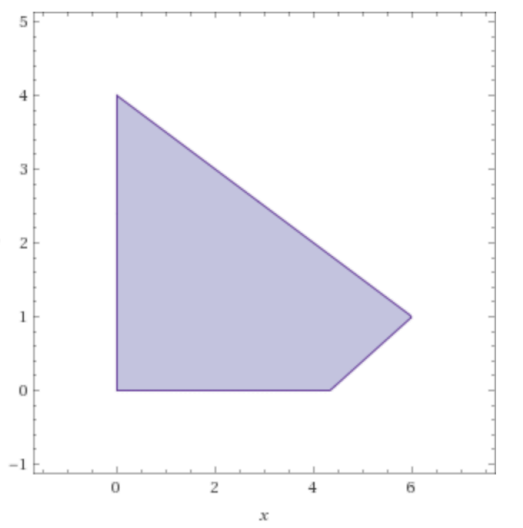
\includegraphics[trim=0cm 0cm 0cm 0cm, clip, width=7cm]{img11.png}
    \caption{Graphical representation of the solution region for the given system of inequalities.}
    \label{fig:img11}
\end{figure}


\subsection{Linear Programming}
Linear programming is a method used in mathematical optimization, where the goal is to maximize or minimize a linear objective function. This method finds applications in diverse fields for optimizing various processes, such as minimizing costs or maximizing profits.
\newline
\textbf{Objective Function:}
The objective function in linear programming is a linear equation of the form:
\[
 z = c_1x_1 + c_2x_2 + \ldots + c_nx_n
\]
where \( c_i \) are coefficients and \( x_i \) are variables.
\newline
\textbf{Constraints:}
The optimization is subject to a set of linear constraints, typically expressed as inequalities. These can be represented as:
\[
 \begin{aligned}
 a_{1,1}x_1 + a_{1,2}x_2 + \ldots + a_{1,n}x_n &\geq h_1 \\
 \vdots \\
 a_{m,1}x_1 + a_{m,2}x_2 + \ldots + a_{m,n}x_n &\leq h_m
 \end{aligned}
\]
\newline
\textbf{Matrix Notation:}
To express the problem in a compact form, we define the following quantities:
\[
 \begin{aligned}
 c &\in \mathbb{R}^n: \text{Coefficient vector} \\
 A &\in \mathbb{R}^{m \times n}: \text{Constraint coefficients matrix} \\
 h &\in \mathbb{R}^m: \text{Constraint values vector} \\
 x &\in \mathbb{R}^n: \text{Solution vector}
 \end{aligned}
\]

\subsubsection{Standard Form of Linear Programming:}
For convenience, we convert all inequalities to either upper bounds (for maximization problems) or lower bounds (for minimization problems), and include non-negativity constraints. The standard forms are:

\textbf{Maximization Problem:}
\[
 \begin{aligned}
 &\text{maximize} \quad z = c^T x \\
 &\text{s.t.} \quad Ax \leq h \\
 &x \geq 0
 \end{aligned}
\]

\textbf{Minimization Problem:}
\[
 \begin{aligned}
 &\text{minimize} \quad z = c^T x \\
 &\text{s.t.} \quad Ax \geq h \\
 &x \geq 0
 \end{aligned}
\]

In these forms, the non-negativity constraint \( x \geq 0 \) is explicitly stated, ensuring that the solution vector \( x \) contains only non-negative values.

\subsubsection{Fundamental Theorem of Linear Programming}
The Fundamental Theorem of Linear Programming provides critical insights into the solution of linear programming problems. It states:

\begin{itemize}
    \item If a linear programming problem has a solution, this solution is guaranteed to occur at a vertex (corner point) of the feasible solution set. This feasible solution set is defined by the constraints of the problem.
    \item In the scenario where multiple solutions exist, at least one of these solutions will be found at a vertex of the feasible solution set. This implies that while multiple solutions might span across the edges of the feasible region, they all intersect at the vertices.
    \item Regardless of whether there is a single solution or multiple solutions, the value of the objective function at these optimal solutions remains unique.
\end{itemize}

%\subsubsection{Graphical Solution of a Linear Program}
A graphical solution method can be effectively used for linear programming problems involving two variables. The steps are as follows:

\begin{enumerate}
    \item Solve the system of inequalities defined by the constraints of the problem.
    \item Identify the feasible region on a plane. This region is a polygonal area where all points satisfy the given constraints. According to the Fundamental Theorem of Linear Programming, at least one optimal solution will be located at a vertex of this feasible region.
    \item Evaluate the objective function at each vertex of the feasible region. Choose the vertex that optimizes (maximizes or minimizes) the value of the objective function. If the feasible region is bounded, both the maximum and minimum values of the objective function can be determined.
\end{enumerate}

Consider the following example of a maximization problem:

\[
 \begin{aligned}
 &\text{maximize} \quad z = 4x + 6y \\
 &\text{s.t.} \quad \\
 &-x + y \leq 11, \\
 &x + y \leq 27, \\
 &2x + 5y \leq 90, \\
 &x, y \geq 0.
 \end{aligned}
\]

This system of inequalities can be rewritten as:

\[
 \begin{cases}
  y \leq x + 11, \\
  y \leq -x + 27, \\
  y \leq -\frac{2}{5}x + 18, \\
  x, y \geq 0.
 \end{cases}
\]

\begin{figure}[H]
    \centering
    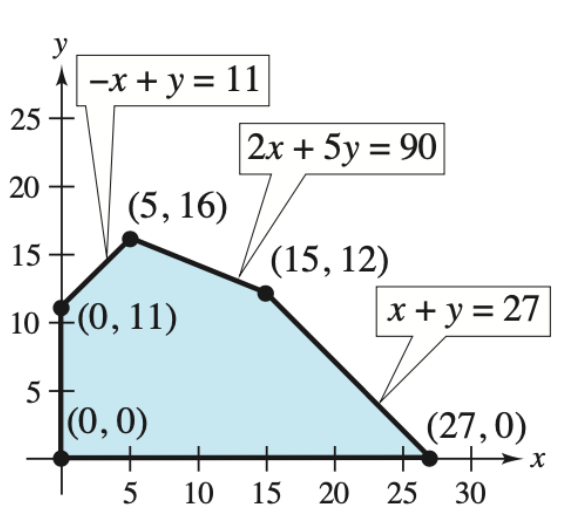
\includegraphics[trim=0cm 0cm 0cm 0cm, clip, width=7cm]{img12.png}
    \caption{Graphical representation of the feasible region.}
    \label{fig:img12}
\end{figure}

To find the optimal solution, evaluate the objective function at each vertex of the feasible region:

\begin{itemize}
    \item At Vertex $(0,0): z=0$,
    \item At Vertex $(0,11): z=66$,
    \item At Vertex $(5,16): z=116$,
    \item At Vertex $(15,12): z=132$ (Optimal),
    \item At Vertex $(27,0): z=108$.
\end{itemize}

The optimal value of the objective function, $z^*$, is achieved at the vertex $(15,12)$.
\subsubsection{Formulating a Problem as Linear Program}
The liquid portion of a diet is to provide at least \textcolor{blue}{300 calories}, \textcolor{red}{36 units of vitamin A}, and \textcolor{orange}{90 units of vitamic C} daily. A cup of dietary drink X provides \textcolor{blue}{60 calories},\textcolor{red}{12 units of vitamin A}, and \textcolor{orange}{10 units of vitamin C}. A cup of dietary drink Y provides \textcolor{blue}{60 calories},\textcolor{red}{6 units of vitamin A}, and \textcolor{orange}{30 units of vitamin C}. Now, suppose that dietary \textcolor{cyan}{drink X cost \$0.12 per cup} and \textcolor{cyan}{drink Y cost \$0.15 per cup}. How many cups of each drink should be conmed each day to minimise the cost and still meet the state daily requirements?
\newline
We obtain the minimization problem:\
\[
 \begin{aligned}
 &\text{min} \quad z = \textcolor{cyan}{0.12}x + \textcolor{cyan}{0.15}y \\
 &\text{s.t.} \quad \textcolor{blue}{60}x + \textcolor{blue}{60}y \geq \textcolor{blue}{300}, \\
 &\textcolor{red}{12}x +\textcolor{red}{6} y \geq \textcolor{red}{36}, \\
 &\textcolor{orange}{10}x + \textcolor{orange}{30}y \geq \textcolor{orange}{90}, \\
 &x, y \geq 0.
 \end{aligned}
\]

\[
 \begin{cases}
  60x +60y \geq 300 \quad \Rightarrow \quad y \geq -x+5 \\
  12x +6y \geq36 \quad \Rightarrow \quad y \geq + -2x+6\\
  10x+30y \leq 90 \quad \Rightarrow \quad y \geq -\frac{1}{3}x+3
  x, y \geq 0.
 \end{cases}
\]

\begin{figure}[H]
    \centering
    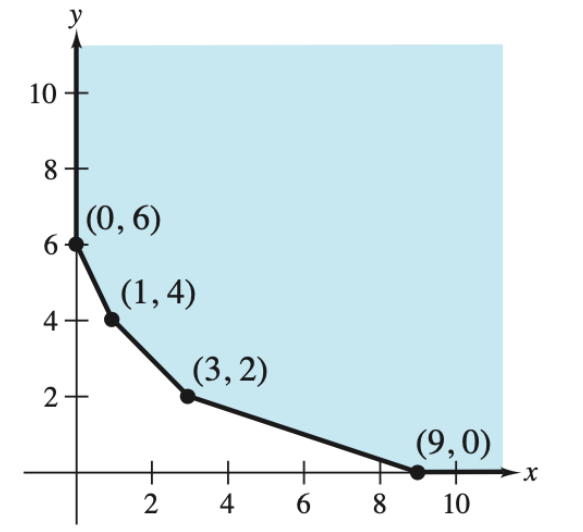
\includegraphics[trim=0cm 0cm 0cm 0cm, clip, width=7cm]{img13.png}
    \caption{Graphical representation of the feasible region.}
    \label{fig:img13}
\end{figure}

To find the optimal solution, evaluate the objective function at each vertex of the feasible region:

\begin{itemize}
    \item At Vertex $(0,6): z=0.90$,
    \item At Vertex $(1,4): z=0.72$,
    \item At Vertex $(3,2): z=0.66$,
    \item At Vertex $(9,0): z=1.08$ ,
\end{itemize}
    The optimal is at Vertex $(3,2): z^*=0.66$.
%%
\subsubsection{The Simplex Method}
The Simplex Method, introduced by George Dantzig in 1947, is an algorithm designed for efficiently solving linear programming problems, especially useful for scenarios with a large number of variables and constraints. However, in the worst-case scenario, the Simplex Method can have exponential complexity due to the potentially enormous number of candidate solutions that need to be examined to find the optimal value.
\newline \newline
\textbf{Formulating the Problem:}
To utilize the Simplex Method, the linear programming problem must first be expressed in standard form. This involves transforming all inequality constraints into equalities by introducing slack variables in a maximization problem or surplus variables in a minimization problem. These additional variables, which have zero coefficients in the objective function, represent the deviation from the constraint's right-hand side value in the optimal solution.
\newline\newline
\textbf{Dimensionality and Variables:}
The coefficient vector is now expanded to \( c \in \mathbb{R}^{n+m} \), where \( m \) is the number of constraints. Similarly, the unknowns vector expands to \( x \in \mathbb{R}^{n+m} \), encompassing both the original variables \( x_1, \ldots, x_n \) and the slack/surplus variables \( s_1, \ldots, s_m \). The coefficient matrix \( A \) also changes accordingly to \( A \in \mathbb{R}^{m \times (n+m)} \).
\newline\newline
\textbf{Algorithm Overview:}
The Simplex Method begins by identifying a basis of the extended coefficient matrix \( A \), which is a square matrix with full rank comprising a mix of original and newly added variables. Variables outside this basis are termed \textit{nonbasic variables}. By setting nonbasic variables to zero, a \textit{basic solution} is derived. It is crucial to verify that all basic solutions satisfy the non-negativity condition to ensure feasibility.
\newline
According to the Fundamental Theorem of Linear Programming, the existence of a feasible solution implies the existence of a feasible basic solution, and likewise, an optimal solution implies the existence of an optimal basic solution. The Simplex algorithm iterates through basic solutions, starting from a feasible one, and progressing towards the optimum. The worst-case number of iterations equals the total number of basic solutions, given by:

\[
 N = \frac{(m+n)!}{m! \cdot n!}.
\]

This number grows exponentially with the increase in variables and constraints, highlighting the potential complexity issue of the Simplex Method. Despite this, under typical conditions, the Simplex Method often reaches the optimal solution in a practical number of iterations.

In summary, the Simplex Method is a powerful tool for solving linear programming problems but requires careful formulation of the problem and an understanding of its potential complexity in scenarios with a large number of variables and constraints.

%%%
\subsubsection{The Simplex Method - Maximization Problem}
For the maximization problem in standard linear programming form, we can introduce slack variables to convert inequality constraints into equalities. From the original set of constraints:

\[
\begin{aligned}
a_{1,1}x_1 + a_{1,2}x_2 + \cdots + a_{1,n}x_n &\leq h_1 \\
\vdots \\
a_{m,1}x_1 + a_{m,2}x_2 + \cdots + a_{m,n}x_n &\leq h_m
\end{aligned}
\]

We transform them to:

\[
\begin{aligned}
a_{1,1}x_1 + a_{1,2}x_2 + \cdots + a_{1,n}x_n + s_1 &= h_1 \\
\vdots \\
a_{m,1}x_1 + a_{m,2}x_2 + \cdots + a_{m,n}x_n + s_m &= h_m
\end{aligned}
\]

Here, \(s_1, s_2, \ldots, s_m\) are the slack variables. The problem is then reformulated as:

\[
c = \begin{bmatrix}
c_1 \\ \vdots \\ c_n \\ 0 \\ \vdots \\ 0
\end{bmatrix},
\quad
x = \begin{bmatrix}
x_1 \\ \vdots \\ x_n \\ s_1 \\ \vdots \\ s_m
\end{bmatrix},
\quad
A = \begin{bmatrix}
a_{1,1} & \cdots & a_{1,n} & 1 & 0 & \cdots & 0 \\
a_{2,1} & \cdots & a_{2,n} & 0 & 1 & \cdots & 0 \\
\vdots & \ddots & \vdots & \vdots & \vdots & \ddots & \vdots \\
a_{m,1} & \cdots & a_{m,n} & 0 & 0 & \cdots & 1
\end{bmatrix},
\quad
h = \begin{bmatrix}
h_1 \\ \vdots \\ h_m
\end{bmatrix}
\]

Additionally, non-negativity constraints are applied to both the decision variables (\(x_1, \ldots, x_n\)) and the slack variables (\(s_1, \ldots, s_m\)).

\subsubsection{The Simplex Method - Minimization Problem}
In the minimization version of a linear programming problem, we address standard form inequalities by introducing \textit{surplus variables}. This transformation converts inequality constraints into equalities, shifting from the original constraints:

\[
\begin{aligned}
a_{1,1}x_1 + a_{1,2}x_2 + \cdots + a_{1,n}x_n &\geq h_1, \\
\vdots \\
a_{m,1}x_1 + a_{m,2}x_2 + \cdots + a_{m,n}x_n &\geq h_m
\end{aligned}
\]

to the following system:

\[
\begin{aligned}
a_{1,1}x_1 + a_{1,2}x_2 + \cdots + a_{1,n}x_n - s_1 &= h_1, \\
\vdots \\
a_{m,1}x_1 + a_{m,2}x_2 + \cdots + a_{m,n}x_n - s_m &= h_m
\end{aligned}
\]

Here, \(s_1, s_2, \ldots, s_m\) are the surplus variables. The problem is then reformulated with the following parameters:

\[
c = \begin{bmatrix}
c_1 \\ \vdots \\ c_n \\ 0 \\ \vdots \\ 0
\end{bmatrix},
\quad
x = \begin{bmatrix}
x_1 \\ \vdots \\ x_n \\ s_1 \\ \vdots \\ s_m
\end{bmatrix},
\quad
A = \begin{bmatrix}
a_{1,1} & \cdots & a_{1,n} & -1 & 0 & \cdots & 0 \\
a_{2,1} & \cdots & a_{2,n} & 0 & -1 & \cdots & 0 \\
\vdots & \ddots & \vdots & \vdots & \vdots & \ddots & \vdots \\
a_{m,1} & \cdots & a_{m,n} & 0 & 0 & \cdots & -1
\end{bmatrix},
\quad
h = \begin{bmatrix}
h_1 \\ \vdots \\ h_m
\end{bmatrix}
\]

Additionally, non-negativity constraints are imposed on both the decision variables (\(x_1, \ldots, x_n\)) and the surplus variables (\(s_1, \ldots, s_m\)).

\subsubsection{Basic and Nonbasic Variables}
In linear programming, the matrix \( A \) can be rearranged by freely swapping its rows and corresponding elements of vector \( h \), and by swapping its columns and corresponding elements of vector \( x \). We partition \( A \) into two sub-matrices:

\[
A = \begin{bmatrix}
    B & D
\end{bmatrix}
\]

Here, \( B \in \mathbb{R}^{mxm} \) consists of \( m \) linearly independent columns from \( A \), ensuring full rank and invertibility. \( D \in \mathbb{R}^{mx(n-m)} \) contains the remaining columns. Similarly, vectors \( x \) and \( c \) are partitioned as:

\[
x = \begin{bmatrix}
    x_B \\
    x_D
\end{bmatrix}, \quad
c = \begin{bmatrix}
    c_B \\
    c_D
\end{bmatrix}
\]

with \( x_B, c_B \in \mathbb{R}^{m} \) and \( x_D, c_D \in \mathbb{R}^{n-m} \).

The constraint system \( Ax = h \) can be rewritten using this decomposition:

\[
Bx_B + Dx_D = h \quad \Rightarrow \quad Bx_B = h - Dx_D
\]

Variables in \( x_B \) are known as \textit{basic variables}, while those in \( x_D \) are \textit{nonbasic variables}.

Inverting the matrix \( B \) (which is always nonsingular due to its full rank), we obtain:

\[
x_B = B^{-1}h - B^{-1}Dx_D
\]

This equation represents a general solution of the problem, with the values of basic variables \( x_B \) depending on the values assigned to the nonbasic variables \( x_D \). Note that \( x_B \) can include both the original unknowns \( x_1, \ldots, x_n \) and the slack variables \( s_1, \ldots, s_m \).

\textbf{Basic Solution:}

A \textit{basic solution} is obtained by setting \( x_D = 0 \):

\[
x_B = B^{-1}h
\]

If the non-negativity condition \( x_B \geq 0 \) is satisfied, the basic solution is feasible. If one or more components of \( x_B \) are zero, the solution is degenerate. Basic solutions correspond to vertices of the feasible region polytope, defined by the intersections of constraints.



\subsubsection{The Simplex Method: Algorithm}
The Simplex method is a systematic procedure for solving linear programming problems. The algorithm can be summarized as follows:

\begin{enumerate}
    \item Convert the given problem into its standard form by adding slack or surplus variables as needed.
    \item Identify a feasible starting basic solution. This can often be achieved by solving an auxiliary problem if a clear starting solution is not immediately apparent.
    \item \textbf{While} the optimality criterion is not met:
    \begin{enumerate}
        \item Apply the iteration rule, which involves exchanging one of the basic variables with a nonbasic variable. This step moves the solution from one vertex of the feasible region to another, seeking to improve the objective function value.
    \end{enumerate}
    \item \textbf{End While}
    \item Return the basic solution that satisfies the optimality criterion.
\end{enumerate}

This method iteratively moves towards the optimal solution by navigating the vertices of the feasible region defined by the constraints.


\subsubsection{Optimal Basic Solution}
The existence of a feasible solution, as stated by the Fundamental Theorem of Linear Programming, guarantees the existence of a feasible basic solution. Similarly, if an optimal solution exists, there must also be an optimal basic solution. The Simplex method navigates through the vertices (corners) of the polytope defined by the constraints of the program until the optimality criterion is met.

\textbf{Downside:} The potential number of basic solutions increases exponentially with the number of variables and constraints. The maximum possible number of iterations can be calculated as:
\[
 N = \frac{(m+n)!}{m!n!}
\]
where \(m\) is the number of constraints and \(n\) is the number of variables.

The optimality condition at each iteration is evaluated using the \textbf{Reduced Cost Coefficients}:
\[
 r_D = c^T_D - c^T_B B^{-1}D
\]
Here, \(c_D\) represents the coefficients of the nonbasic variables in the objective function, \(c_B\) represents the coefficients of the basic variables, \(B^{-1}\) is the inverse of the basic matrix, and \(D\) is the matrix of nonbasic columns.

The optimality conditions for the Simplex method are:
\begin{itemize}
    \item \textbf{Maximization:} \( r_D \leq 0 \)
    \item \textbf{Minimization:} \( r_D \geq 0 \)
\end{itemize}

\textbf{Iterative Rule:}
If the optimality condition is not satisfied, select the variable with the highest (for maximization) or lowest (for minimization) reduced cost coefficient \( r_D \) to enter the basis. Determine the departing variable by calculating the ratio:
\[
 \frac{B^{-1}h}{B^{-1}D}
\]
for the column associated with the entering variable and select the variable with the smallest \textbf{positive} value. This step ensures the maintenance of a feasible solution while seeking improvement in the objective function value.
\subsubsection{Feasible Starting Basic Solution: Auxiliary Problem}
To initiate the Simplex method, a feasible starting basic solution is required, which is typically obtained by solving an \textbf{auxiliary problem}. The initial step involves ensuring that all the elements of the right-hand side vector \(h\) are positive. This condition is achieved by either adding slack variables or subtracting surplus variables to/from the original constraints, ensuring \(h_i \geq 0\) for all \(i\).

The constraints are modified as follows:

\[
\begin{aligned}
a_{1,1}x_1 + a_{1,2}x_2 + \cdots + a_{1,n}x_n \pm s_1 &= h_1, \\
\vdots \\
a_{m,1}x_1 + a_{m,2}x_2 + \cdots + a_{m,n}x_n \pm s_m &= h_m,
\end{aligned}
\]

where the sign of \(s_i\) is chosen to ensure non-negativity of \(h_i\).

To construct the auxiliary problem, we add artificial variables \(u_1, \ldots, u_m\) to each constraint:

\[
\begin{aligned}
a_{1,1}x_1 + a_{1,2}x_2 + \cdots + a_{1,n}x_n \pm s_1 + u_1 &= h_1, \\
\vdots \\
a_{m,1}x_1 + a_{m,2}x_2 + \cdots + a_{m,n}x_n \pm s_m + u_m &= h_m.
\end{aligned}
\]

The auxiliary problem's objective function is then defined as the sum of these artificial variables:

\[
 z_{aux} = u_1 + u_2 + \cdots + u_m.
\]

This auxiliary problem is inherently a \textbf{minimization} problem. The initial feasible basic solution corresponds to the case where \(z_{aux} = 0\). If \(z_{aux}\) cannot be minimized to zero, it implies that neither the auxiliary problem nor the original linear programming problem has a feasible solution.

% \subsubsection{Simplex Method: Minimization}
% Let us consider the following linear programming problem:
%
%
% \[
%  \begin{aligned}
%  &\text{min} \quad z = 9x_1 + 11x_2 +8x_3 \\
%  &\text{s.t.} \quad \\
%  & 2x_1 + 2x_2 +3x_3\geq 210, \\
%  & 3x_1+4x_2+2x_3\geq 360, \\
%  & x_1,x_2,x_3 \geq 0
%  \end{aligned}
% \]
% The problem is already in standard form for a minimization so we can directly subtract the surplus variables to turn the inequalities into equalities contraints.
%
% after substracting the surplus variables, the problem becomes:
% \[
%  \begin{aligned}
%  &\text{min} \quad z = 9x_1 + 11x_2 +8x_3 \\
%  &\text{s.t.} \quad \\
%  & 2x_1 + x_2 +3x_3 -s_1 = 210, \\
%  & 3x_1+ 4x_2 +2x_3 -s_2=  360, \\
%  & x_1,x_2,x_3 \geq 0; \quad s_1,s_2\geq0
%  \end{aligned}
% \]
%
% \[
% c = \begin{bmatrix}
% 9 \\11 \\ 8\\0\\0
% \end{bmatrix},
% \quad
% x = \begin{bmatrix}
% x_1 \\ x_2 \\ x_3 \\ s_1  \\ s_2
% \end{bmatrix},
% \quad
% A = \begin{bmatrix}
% 2 & 1& 3& -1&0 \\
% 3 & 4 & 2 & 0 & -1
% \end{bmatrix},
% \quad
% h = \begin{bmatrix}
% 210 \\ 360
% \end{bmatrix}
% \]
%
% we can split the matrices in the following basic variables:
%
% \[
% c_B = \begin{bmatrix}
% 8 \\ 0
% \end{bmatrix},
% \quad
% x_B = \begin{bmatrix}
% x_3 \\ s_1
% \end{bmatrix},
% \quad
% B = \begin{bmatrix}
% 3 & -1 \\
% 2 & 0
% \end{bmatrix},
% \quad
% h = \begin{bmatrix}
% 210 \\ 360
% \end{bmatrix}
% \]
% and nonbasic variables:
%
%
% \[
% c_D = \begin{bmatrix}
% 8 \\11 \\ 0
% \end{bmatrix},
% \quad
% x_D = \begin{bmatrix}
% x_1 \\ x_2 \\ s_2
% \end{bmatrix},
% \quad
% B = \begin{bmatrix}
% 2 & 1 & 0 \\
% 3 & 4 & -1
% \end{bmatrix}
% \]
%
% We obtain the following basic solution (remeber to set $x_D =0$):
% \[
%  x_B=B^{-1}h-B^{-1}Dx_D= \begin{bmatrix}
%                           0 & 0.5 \\
%                           -1 & 1.5
%                          \end{bmatrix}
%                          \begin{bmatrix}
%                           210 \\
%                           360
%                          \end{bmatrix}
%                          =
%                          \begin{bmatrix}
%                           180\\
%                           330
%                          \end{bmatrix}
%
% \]
% which is feasible since also the non negativity constraint is satisfied. The correspodning value of the objective function is given by:
% \[
%  z = c^T_Bx_B = \begin{bmatrix}
%                  8 & 0
%                 \end{bmatrix}
%                 \begin{bmatrix}
%                  180 & 330
%                 \end{bmatrix}
%                 = 1440
% \]
%
% is the solution optimal?
% let apply the simplex method to find it out.
%
% we start by computing the reduced coeffiecints
% \[
%  r_D = c^T_D - c^T_BB^{-1}D=\begin{bmatrix}
%                              9 & 11 & 0
%                             \end{bmatrix}
%                             -
%                             \begin{bmatrix}
%                              8 & 0
%                             \end{bmatrix}
%                             \begin{bmatrix}
%                              1.5 & 2 & -0.5 \\
%                              2.5 & 5 & -1/5
%                             \end{bmatrix}
%                             =
%                             \begin{bmatrix}
%                              -3 & -5 & 4
%                             \end{bmatrix}
%
%
%
% \]
%
% According to the iterative rule, we pick the coffeicint with the smallest value, since we are dealing with a minimization (-5 in this case). in othber words, the entiring variable will be $x_2$ since - according to the algorithm - it should improve the vlaue of the obkective function.
%
% which should be the deprting variable?
% we keep applying the iterative tule by computing the ratios for the second column: \[
%                                                                                     \frac{B^{-1}h}{B^{-1}D} = \begin{bmatrix}
%                                                                                                                90 \\ 66
%                                                                                                               \end{bmatrix}
%
%                                                                                    \]
%                                                                                    and by sleecting the smallest positive value (in this case 66). The correspoding variable is $s_1$ whihc will now leaving the basis.
%
%                                                                                    How is our new system (basic and nonbasic) defined?
%
%                                                                                    The basic variables are
% \[
% c_B = \begin{bmatrix}
% 8 \\ 11
% \end{bmatrix},
% \quad
% x_B = \begin{bmatrix}
% x_3 \\ x_2
% \end{bmatrix},
% \quad
% B = \begin{bmatrix}
% 3 & -1 \\
% 2 & 4
% \end{bmatrix},
% \quad
% h = \begin{bmatrix}
% 210 \\ 360
% \end{bmatrix}
% \]
%
% while the non basic variables are
% \[
% c_D = \begin{bmatrix}
% 9 \\ 0 \\ 0 \\0
% \end{bmatrix},
% \quad
% x_D = \begin{bmatrix}
% x_1 \\ s_1 \\ s_2
% \end{bmatrix},
% \quad
% D = \begin{bmatrix}
% 2 & -1 & 0 \\
% 3 & 0 & -1
% \end{bmatrix},
% \]
%
% we obtain the following basic solution (remeber to set $x_D=0$)
% \[
%  x_B=B^{-1}h-B^{-1}Dx_D = \begin{bmatrix}
%                            0.4& -0.1 \\
%                            -0.2 & 0.33
%                           \end{bmatrix}
%                           \begin{bmatrix}
%                            210 \\
%                            360
%                           \end{bmatrix}
%                           =
%                           \begin{bmatrix}
%                            48\\66
%                           \end{bmatrix}
%
%
%
% \]
% whihc is again feasible as guaranteed by the algorithm The correspodnign value of the objective function is given by
% \[
%  z = c^T_Bx_B=\begin{bmatrix}
%                8 & 11
%               \end{bmatrix}
%               \begin{bmatrix}
%                48 \\ 66
%               \end{bmatrix}
%               = 1100
%
%
% \]
%
% The value is lower thna the one obtained before (1440) so the objective function value is improving. let us check if it is the otpimal solution by computing the reduced cost coeffiecints. The reduced cost coeffiect are given by
% \[
%  r_D= c_D^T-c_B^TB^{-1}D = \begin{bmatrix}
%                             9 & 0 & 0
%                            \end{bmatrix}
%                            -
%                            \begin{bmatrix}
%                             8 & 11
%                            \end{bmatrix}
%                            \begin{bmatrix}
%                             0.5 & -0.4 & 0.1 \\
%                             0.5 & 0.2 & -0.33
%                            \end{bmatrix}
%                            =
%                            \begin{bmatrix}
%                             -0.5  & 1 & 2.5
%                            \end{bmatrix}
% \]
% The solution is still not optimal since we have a negative reduced cost coeffiecint. The entiering variable will be $x_1$, which corresponds to the only n egative value (-0.5)
%
% whihc should be the departing variable?
% we keep applying the iterative rule by computing the ratios for the first column
% \[
%  \frac{B^{-1}h}{B^{-1}D} = \begin{bmatrix}
%                             96 // 132
%                            \end{bmatrix}
%
% \]
% and by selecting the smallest positive value (int his case 96). the correspoding variable is $x_3$ which will be now leaving the basis.
%
% How is our new system (basic and non basic variables) defined?
%                                                                                The basic variables are
% \[
% c_B = \begin{bmatrix}
% 9 \\ 11
% \end{bmatrix},
% \quad
% x_B = \begin{bmatrix}
% x_1 \\ x_2
% \end{bmatrix},
% \quad
% B = \begin{bmatrix}
% 2 & -1 \\
% 3 & 4
% \end{bmatrix},
% \quad
% h = \begin{bmatrix}
% 210 \\ 360
% \end{bmatrix}
% \]
%
% while the non basic variables are
% \[
% c_D = \begin{bmatrix}
% 8 \\ 0 \\ 0
% \end{bmatrix},
% \quad
% x_D = \begin{bmatrix}
% x_3 \\ s_1 \\ s_2
% \end{bmatrix},
% \quad
% D = \begin{bmatrix}
% 3 & -1 & 0 \\
% 2 & 0 & -1
% \end{bmatrix},
% \]
%
% we obtain the following basic solution (remeber to set $x_D=0$)
% \[
%  x_B=B^{-1}h-B^{-1}Dx_D = \begin{bmatrix}
%                            0.8& -0.2 \\
%                            -0.66 & 0.4
%                           \end{bmatrix}
%                           \begin{bmatrix}
%                            210 \\
%                            360
%                           \end{bmatrix}
%                           =
%                           \begin{bmatrix}
%                            96\\18
%                           \end{bmatrix}
%
%
%
% \]
%
% whihc is again feasible as guaranteed by the algorithm The correspodnign value of the objective function is given by
% \[
%  z = c^T_Bx_B=\begin{bmatrix}
%                9 & 11
%               \end{bmatrix}
%               \begin{bmatrix}
%                96 \\ 18
%               \end{bmatrix}
%               = 1062
%
%
% \]
%
% WE obtained an even lower value of the objective function (1062 < 1100). can we still do better or we reached the otpimal soluton?
%
% the reduced cost coefficient are given by
% \[
%  r_D= c&T_D-c^T_BB^{-1}D = \begin{bmatrix}
%                             9 & 0 & 0
%                            \end{bmatrix}
%                            -
%                            \begin{bmatrix}
%                             9 & 11
%                            \end{bmatrix}
%                            \begin{bmatrix}
%                             2 & -0.8 & 0.2 \\
%                             -1 & 0.66 & -0.4
%                            \end{bmatrix}
%                            \begin{bmatrix}
%                             1 & 0.6 & 2.6
%                            \end{bmatrix}
%
%
%
%
% \]
%
%
% all theredued cost coefficnt are postive and the algorithm stops: the simpex metho converged to the otpimal solution:
% \[
%  x^*=\begin{bmatrix}
%       96 \\ 18 \\ 9
%      \end{bmatrix}
%      with z^*=1062
%
% \]

\subsubsection{Simplex Method: Minimization Example}
Consider the following linear programming problem for minimization:

\[
 \begin{aligned}
 &\text{min} \quad z = 9x_1 + 11x_2 + 8x_3, \\
 &\text{s.t.} \\
 & 2x_1 + 2x_2 + 3x_3 \geq 210, \\
 & 3x_1 + 4x_2 + 2x_3 \geq 360, \\
 & x_1, x_2, x_3 \geq 0.
 \end{aligned}
\]

To transform inequalities into equalities, surplus variables are subtracted:

\[
 \begin{aligned}
 & 2x_1 + 2x_2 + 3x_3 - s_1 = 210, \\
 & 3x_1 + 4x_2 + 2x_3 - s_2 = 360, \\
 & x_1, x_2, x_3, s_1, s_2 \geq 0.
 \end{aligned}
\]

Vectors and matrices are defined as:

\[
c = \begin{bmatrix} 9 \\ 11 \\ 8 \\ 0 \\ 0 \end{bmatrix}, \quad
x = \begin{bmatrix} x_1 \\ x_2 \\ x_3 \\ s_1 \\ s_2 \end{bmatrix}, \quad
A = \begin{bmatrix} 2 & 2 & 3 & -1 & 0 \\ 3 & 4 & 2 & 0 & -1 \end{bmatrix}, \quad
h = \begin{bmatrix} 210 \\ 360 \end{bmatrix}.
\]

Separating into basic (\(B\)) and non-basic (\(D\)) components:

\[
c_B = \begin{bmatrix} 8 \\ 0 \end{bmatrix}, \quad
x_B = \begin{bmatrix} x_3 \\ s_1 \end{bmatrix}, \quad
B = \begin{bmatrix} 3 & -1 \\ 2 & 0 \end{bmatrix}, \quad
h = \begin{bmatrix} 210 \\ 360 \end{bmatrix},
\]

\[
c_D = \begin{bmatrix} 9 \\ 11 \\ 0 \end{bmatrix}, \quad
x_D = \begin{bmatrix} x_1 \\ x_2 \\ s_2 \end{bmatrix}, \quad
D = \begin{bmatrix} 2 & 1 & 0 \\ 3 & 4 & -1 \end{bmatrix}.
\]

Computing the basic solution with \(x_D = 0\):

\[
x_B = B^{-1}h = \begin{bmatrix} 0.5 & -0.25 \\ -0.5 & 0.75 \end{bmatrix} \begin{bmatrix} 210 \\ 360 \end{bmatrix} = \begin{bmatrix} 180 \\ 330 \end{bmatrix}.
\]

This feasible solution has an objective function value of \(z= c^T_Bx_B = 1440\). To determine if it is optimal, compute the reduced cost coefficients:

\[
r_D = c^T_D - c^T_BB^{-1}D = \begin{bmatrix} -3 & -5 & 4 \end{bmatrix}.
\]

Since there are negative coefficients in \(r_D\), the solution is not optimal for a minimization problem. The entering variable is \(x_2\), corresponding to the smallest value in \(r_D\). For the departing variable, calculate the ratios:

\[
\frac{B^{-1}h}{B^{-1}D} = \begin{bmatrix} 90 \\ 66 \end{bmatrix}.
\]

Selecting the smallest positive value indicates \(s_1\) as the departing variable. Reformulating the basic and non-basic variables:

\[
c_B = \begin{bmatrix} 8 \\ 11 \end{bmatrix}, \quad
x_B = \begin{bmatrix} x_3 \\ x_2 \end{bmatrix}, \quad
B = \begin{bmatrix} 3 & 1 \\ 2 & 4 \end{bmatrix},
\]

\[
c_D = \begin{bmatrix} 9 \\ 0 \\ 0 \end{bmatrix}, \quad
x_D = \begin{bmatrix} x_1 \\ s_1 \\ s_2 \end{bmatrix}, \quad
D = \begin{bmatrix} 2 & -1 & 0 \\ 3 & 0 & -1 \end{bmatrix}.
\]

The new basic solution yields \(x_B = \begin{bmatrix} 48 \\ 66 \end{bmatrix}\) with \(z = 1100\). Further iterations involve computing new \(r_D\), identifying entering and departing variables, and recalculating \(x_B\) until all reduced cost coefficients are non-negative, indicating an optimal solution has been found.

\subsection{Project 5}
\subsubsection{Project 5 - Graphical Solution of Linear Pogramming Problems}
\begin{enumerate}
	\item[(1)] \begin{equation*}
		\begin{aligned}
		& \text{min}  &  z=4x&+y\\
		& \text{ s.t.} &  x+2y &\leq 40 \\
		& &   x+y &\geq 30\\
		& &   2x+3y &\geq 72 \\
		& &  x,\,y &\geq0 \\
		\end{aligned}
		\end{equation*}
	\item[(2)] A tailor plans to sell two types of trousers, with production costs of 25 CHF and 40 CHF, respectively. The former type can be sold for 85 CHF, while the latter for 110 CHF. The tailor estimates a total monthly demand of 265 trousers. Find the number of units of each type of trousers that should be produced in order to maximise the net profit of the tailor, if we assume that the he cannot spend more than 7000 CHF in raw materials.
\end{enumerate}
Start by writing problem (2) as a linear programming problem. Then complete the following tasks:
\begin{itemize}
	\item Solve the system of inequalities.
	\item Plot the feasible region identified by the constraints.
	\item Find the optimal solution and the value of the objective function in that point.
\end{itemize}

\subsection{Solve the system of inequalities.}
1. \newline
\begin{equation*}
		\begin{aligned}
		& \text{min}  &  z=4x&+y\\
		& \text{ s.t.} &  x+2y &\leq 40 \\
		& &   x+y &\geq 30\\
		& &   2x+3y &\geq 72 \\
		& &  x,\,y &\geq0 \\
		\end{aligned}
\end{equation*}


\begin{figure}[H]
    \centering
    % Trim 5cm from each side and clip the image
    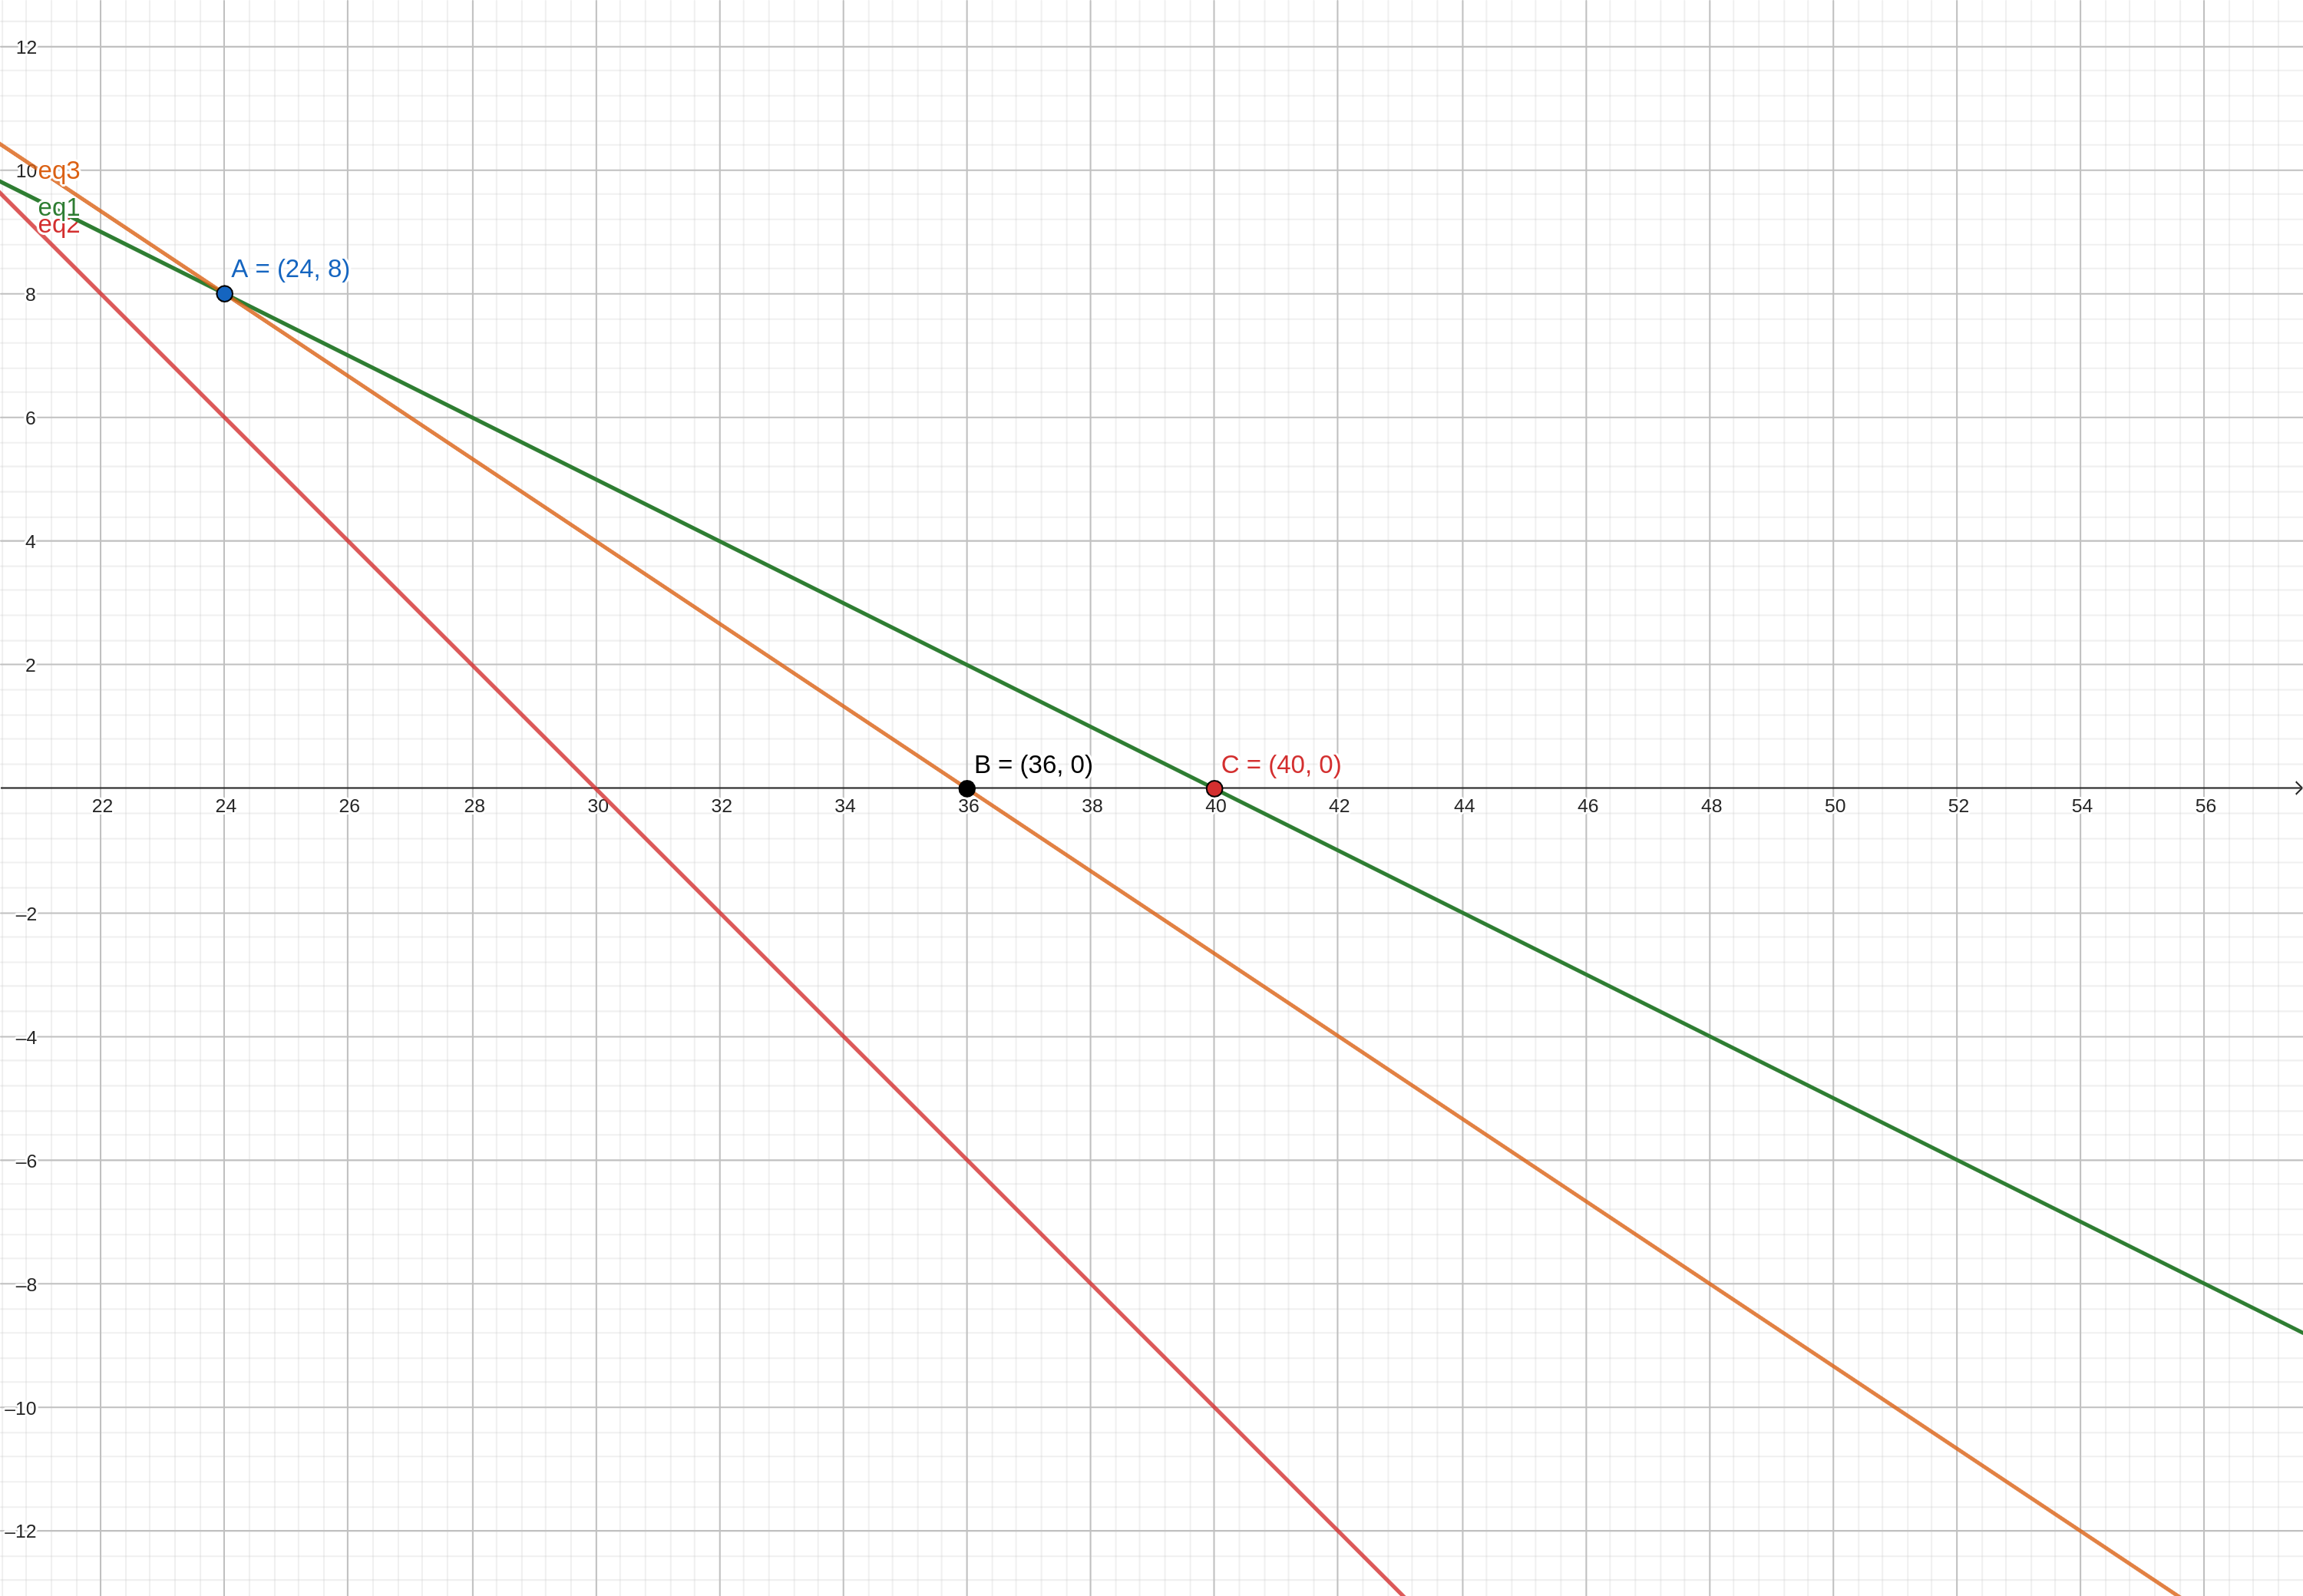
\includegraphics[trim=0cm 10cm 10cm 2cm, clip, width=\textwidth]{geogebra-export.png}
    \caption{Graphical Illustration of the equations with geogebra.}
    \label{fig:img1}
\end{figure}

In Figure \ref{fig:img1}, the graphical representation of each inequality constraint has been transformed into its equivalent equality for visualization purposes. The line for the inequality $x + 2y \leq 40$ is accompanied by shading in the area below it, whereas for the inequalities $x + y \geq 30$ and $2x + 3y \geq 72$, shading is applied above their respective lines.

The intersections of these lines form the vertices of the feasible region, identifiable as points:
\begin{itemize}
 \item $A = (24, 8)$
 \item $B = (36, 0)$
 \item $C = (40, 0)$
\end{itemize}

To determine the minimum value of $z$, the equation $z = 4x + y$ is solved at each of these points.


For A = (24, 8) \newline
\begin{equation*}
		\begin{aligned}
 z_1 = 4 (24) + 1 (8) \\
 z_1 = 96 + 8 \\
 z_1 = 104 \\
 		\end{aligned}
\end{equation*}
\newline
For A = (36, 0)
\newline
\begin{equation*}
		\begin{aligned}
 z_1 = 4 (36) + 1 (0) \\
 z_1 =  144 + 0 \\
 z_1 = 144\\
 		\end{aligned}
\end{equation*}
\newline
For A = (40, 0)
\newline
\begin{equation*}
		\begin{aligned}
 z_1 = 4 (40) + 1 (0) \\
 z_1 =  160 + 0 \\
 z_1 = 160	\\
 		\end{aligned}
\end{equation*}
\newline

The minimum value achieved for $z$ is \textbf{$z_1 = 104$}.

\bigskip
\noindent 2. \newline
Consider $x$ as the quantity of the first type of trousers and $y$ as the quantity of the second type. The tailor's objective is to maximize the net profit, which is calculated as the difference between the selling price and the production cost.

\medskip
\noindent The net profit per unit for the first type of trousers is calculated as:
\[ 85 - 25 = 60 \text{ CHF per unit} \]

\noindent Similarly, the net profit per unit for the second type of trousers is:
\[ 110 - 40 = 70 \text{ CHF per unit} \]

\noindent Consequently, the objective function to be maximized is:
\[ z = 60x + 70y \]


The constraints:
\begin{itemize}
 \item Estimate total monthly demand is: $x+y \leq 265$
 \item Budget for raw materials: $25x + 40y \leq 7000 chf$
 \item Non-negativity: $x \geq 0 \quad y \geq 0$
\end{itemize}

\begin{equation*}
		\begin{aligned}
		& \text{max}  &  z=60x + 70y\\
		& \text{s.t.} &  x+y \leq 265\\
		& &   25x+40y \leq 7000 \\
		& &  x,\,y \geq0 \\
		\end{aligned}
\end{equation*}


\begin{figure}[H]
    \centering
    % Trim 5cm from each side and clip the image
    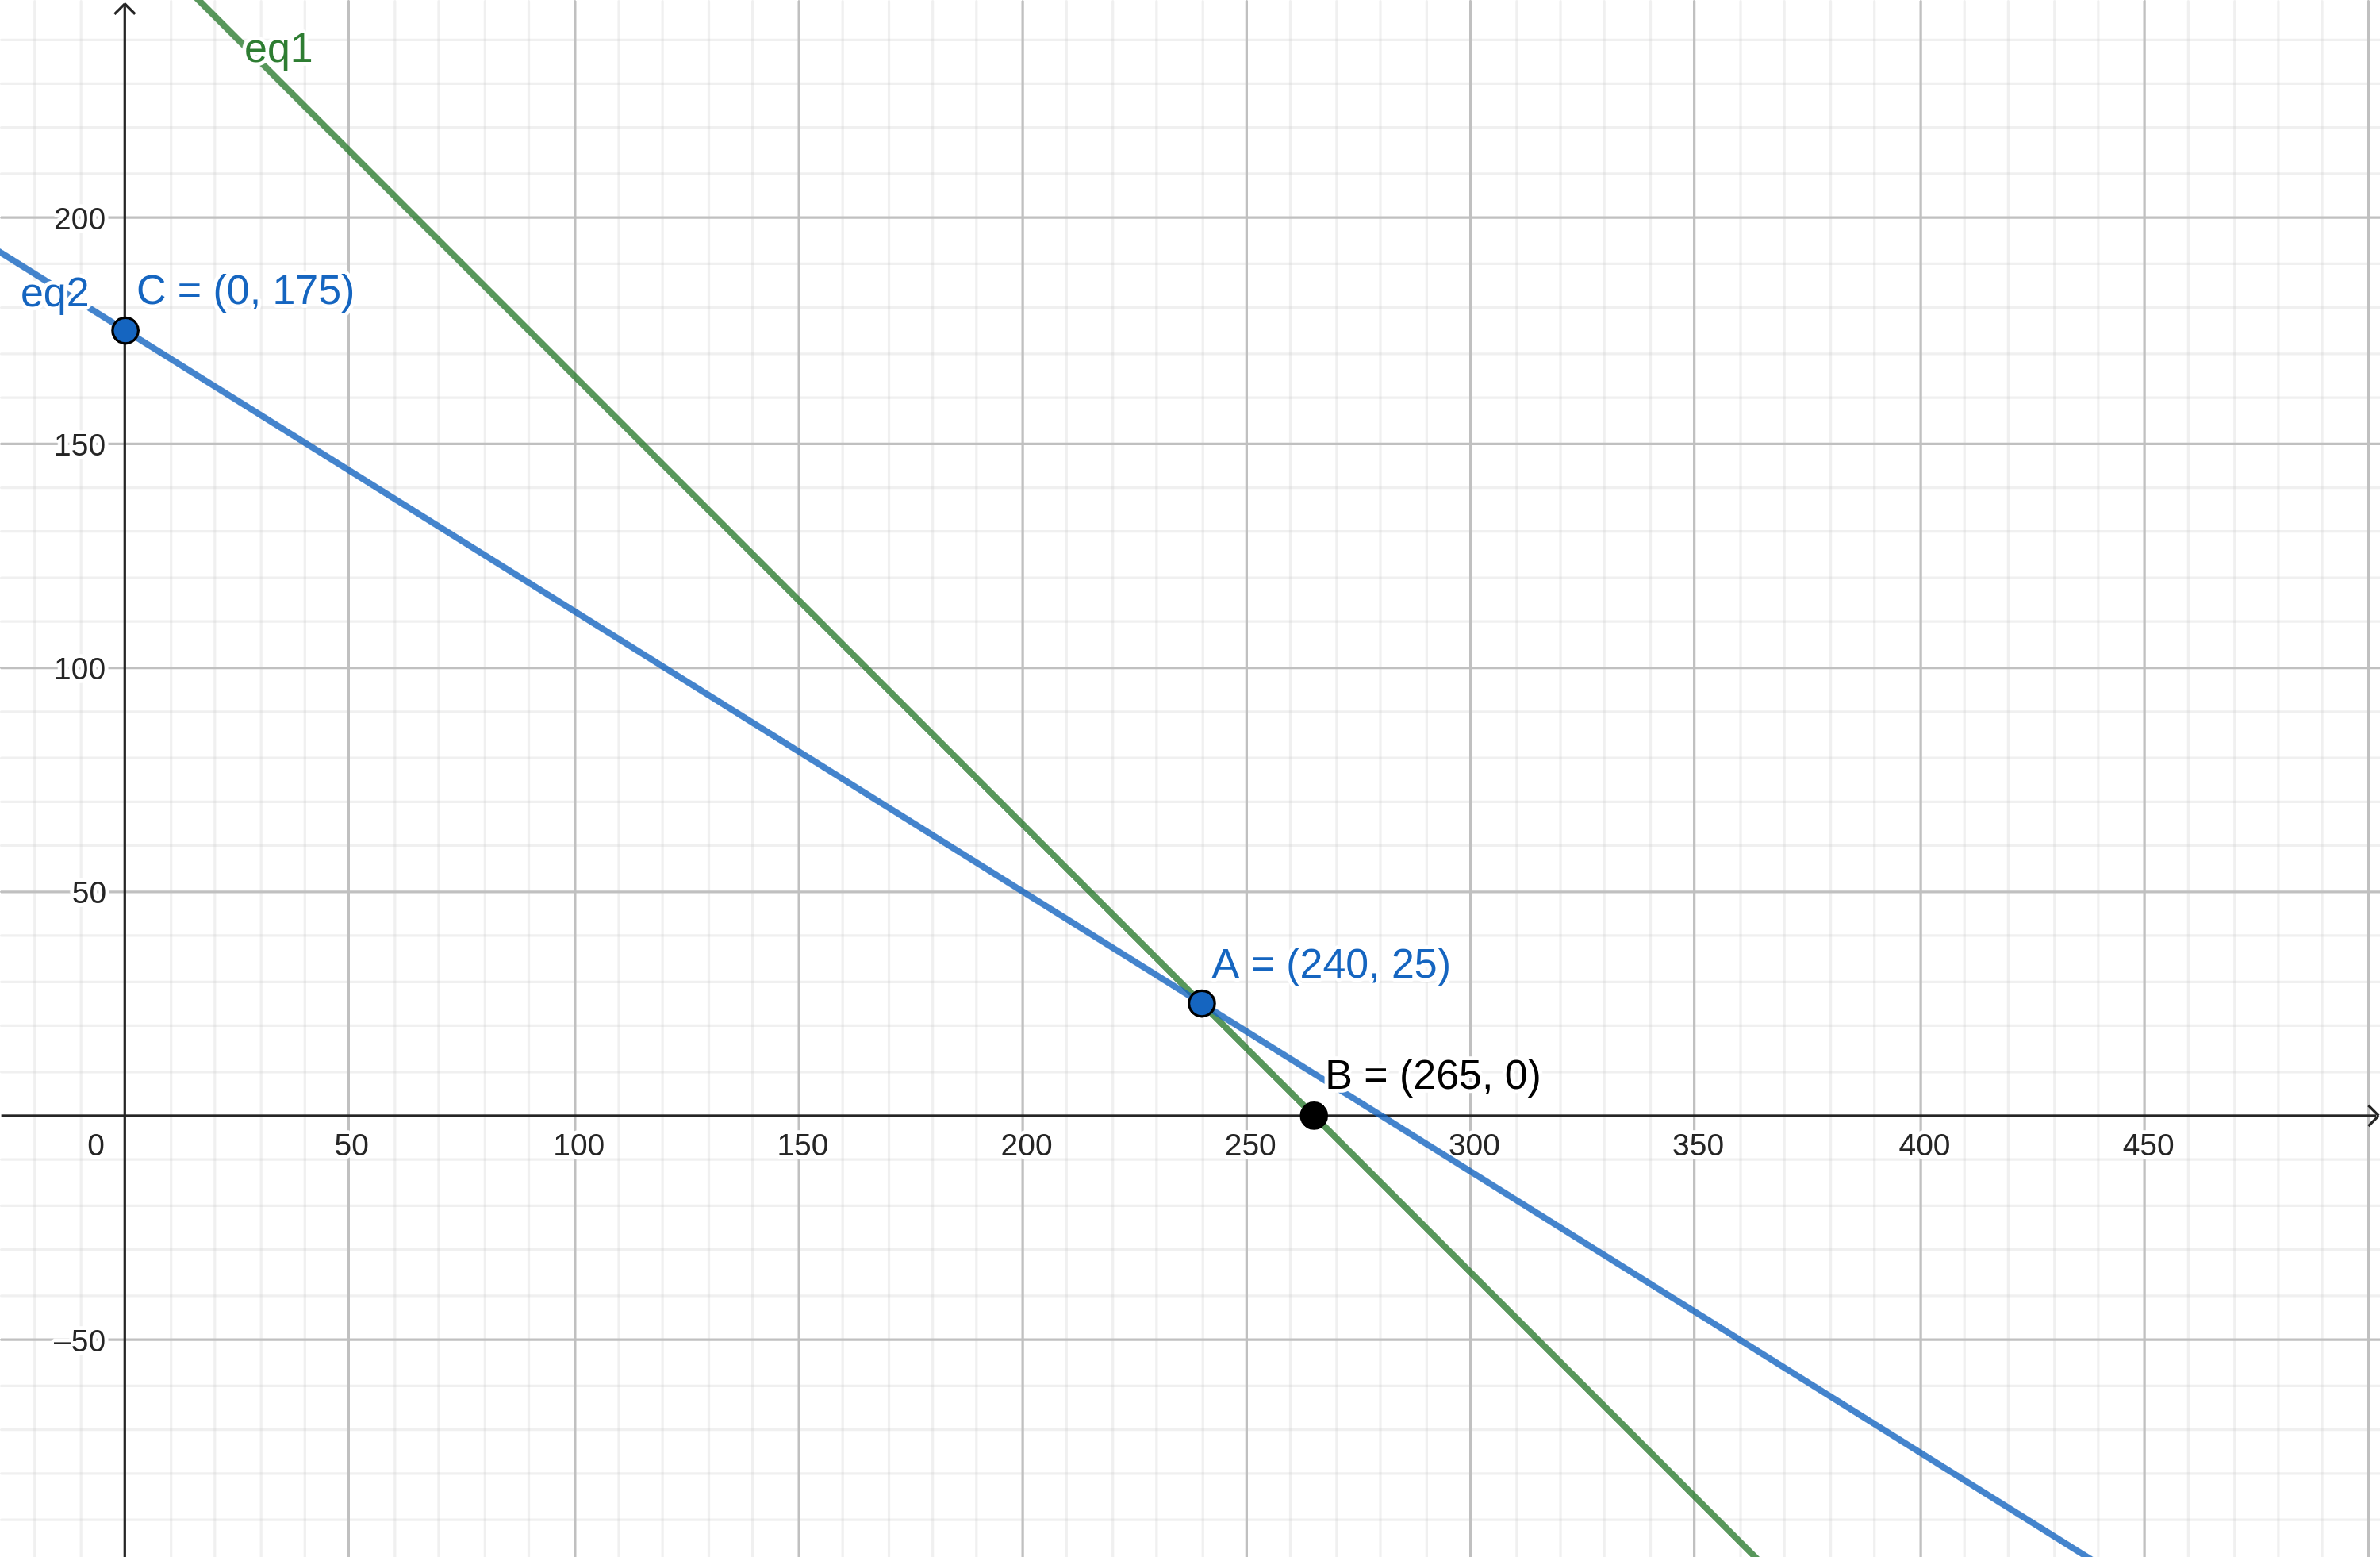
\includegraphics[trim=0cm 10cm 10cm 2cm, clip, width=\textwidth]{geogebra-export2.png}
    \caption{Graphical Illustration of the equations with geogebra.}
    \label{fig:img2}
\end{figure}
It is possibile to get three points on the vertices of the feasibile region: \newline
\begin{itemize}
 \item $A = (240, 25)$
 \item $B = (265, 0)$
 \item $C = (0, 175)$
\end{itemize}

It is possibile to find the minimum z from all the points trough solving the $z = 60x + 70y$.
\newline

For A = (240, 25) \newline
\begin{equation*}
		\begin{aligned}
 z_1 = 60 (240) + 70 (25) \\
 z_1 = 14400 + 1750 \\
  z_1 = 16150\\
 		\end{aligned}
\end{equation*}
\newline
For A = (265, 0)
\newline
\begin{equation*}
		\begin{aligned}
 z_1 = 60 (265) + 70 (0) \\
 z_1 =  15900 \\
 		\end{aligned}
\end{equation*}
\newline
For A = (280, 0)
\newline
\begin{equation*}
		\begin{aligned}
 z_1 = 60 (0) + 70 (175) \\
 z_1 =  12250 \\
		\end{aligned}
\end{equation*}
\newline
The Minimum of Z is \textbf{$z_1 = 16150$}.
\newline\newline

\subsection{Project 5 - Implementation of the Simplex Method}
SimplexSolve.m - which solves a maximisation or minimisation problem using the simplex method.
\begin{lstlisting}
 function [x_B,c_B,index_B] = simplexSolve (type,B,D,c_B,c_D,h,x_B,x_D,index_B,index_D,itMax)
% Solving a maximization problem with the simplex method

% Initialize the number of iterations
nIter = 0;

% Compute B^{-1}*D and B^{-1}*h
BiD = B\D;
Bih = B\h;

% Compute the reduced cost coefficients
r_D = c_D - c_B * BiD;

tol = max(size(r_D)); % the optimality condition is satisfied if all reduced cost coefficients are positive or negative (depending on the problem)

% Check the optimality condition, in order to skip the loop if the solution is already optimal)
if(strcmp(type,'max'))
    optCheck = sum(r_D <= 0);
elseif(strcmp(type,'min'))
    optCheck = sum(r_D >= 0);
else
    error('Incorrect type specified. Choose either a maximisation (max) or minimisation (min) problem.')
end

while(optCheck~=tol)

    % TODO: Find the index of the entering variable
    if(strcmp(type,'max'))
        [~, idxIN]= max(r_D);
    elseif(strcmp(type,'min'))
        [~, idxIN] = min(r_D);
    else
        error('Incorrect type specified. Choose either a maximisation (max) or minimisation (min) problem.')
    end

    in = D(:,idxIN);
    c_in = c_D(1,idxIN);
    index_in = index_D(1,idxIN);

    % Evaluate the coefficients ratio for the column corresponding to the entering variable
    ratio = Bih ./ BiD(:, idxIN);

    % Find the smallest positive ratio
    idxOUT = find(ratio == min(ratio(ratio >= 0)), 1);
    out = B(:,idxOUT);
    c_out = c_B(1,idxOUT);
    index_out = index_B(1,idxOUT);

    % Update the matrices by exchanging the columns
    B(:,idxOUT) = in;
    D(:,idxIN) = out;
    c_B(1,idxOUT) = c_in;
    c_D(1,idxIN) = c_out;
    index_B(1,idxOUT) = index_in;
    index_D(1,idxIN) = index_out;

    % Compute B^{-1}*D and B^{-1}*h
    BiD = B\D;
    Bih = B\h;

    % Compute the reduced cost coefficients
    r_D = c_D - c_B * BiD;

    %  Check the optimality condition
    if(strcmp(type,'max'))
        optCheck = sum(r_D <= 0);
    elseif(strcmp(type,'min'))
        optCheck = sum(r_D >= 0);
    else
        error('Incorrect type specified. Choose either a maximisation (max) or minimisation (min) problem.')
    end

    % Detect inefficient looping if nIter > total number of basic solutions
    nIter = nIter + 1;
    if(nIter>itMax)
       error('Incorrect loop, more iterations than the number of basic solutions');
    end

    % compute the new x_B
    x_B = Bih - BiD*x_D;


    fprintf('x_B: %d \n', x_B);


end

end
\end{lstlisting}

simplex.m - is a wrapper which calls all the functions necessary to find a solution to the linear program.
\begin{lstlisting}
 function [z,x_B,index_B] = simplex (type,A,h,c,sign)
% Simplex method solver for a linear programming problem
% Input arguments:
%   type = 'max' for maximization, 'min' for minimization
%   A    = matrix holding the constraints coefficients
%   h    = coefficients of the constraints inequalities (rhs vector)
%   c    = coefficients of the objective function
%   sign = vector holding information about the constraints if the system
%          needs to be standardized (-1: less or equal, 0: equal, 1:vgreater or equal)

m = size(A,1);
n = size(A,2);

% Compute the maximum number of basic solutions of the original problem (i.e., the maximum number of iterations necessary to solve the problem)
itMax = nchoosek(m+n, n);
% Writing the problem in standard form
[A_aug,h,c_aug] = standardize(type,A,h,c,m,sign);

% Determining a starting feasible initial basic solution
[B,D,c_B,c_D,x_B,x_D,index_B,index_D] = auxiliary(A_aug,c_aug,h,m,n);

% Solving the linear programming problem with the Simplex method
[x_B,c_B,index_B] = simplexSolve(type,B,D,c_B,c_D,h,x_B,x_D,index_B,index_D,itMax);

% Compute the value of the objective function
z = round(c_B * x_B);

% Output of the solution
[x_B,index_B] = printSol(z,x_B,index_B,m,n);

end
\end{lstlisting}

standardize.m - which writes a maximisation or minimisation input problem in standard form.
\begin{lstlisting}
 function [A_aug,h,c_aug] = standardize(type,A,h,c,m,sign)
% return arguments are:
% (1) A_aug = augmented matrix A, containing also the surplus and slack variables
% (2) c_aug = augmented coefficients vector c (check compatibility of dimensions with A)
% (3) h, right hand side vector (remember to flip the signs when changing the inequalities)

aug_matrix = eye(m); % matrix corresponding to the slack/surplus variables

if(strcmp(type,'max'))
    for i = 1:m
        if(sign(i)==1)
            % Using a surplus instead of a slack variable
            aug_matrix(i,:) = -aug_matrix(i,:);
        end
    end
elseif(strcmp(type,'min'))
    for i = 1:m
        if(sign(i)==-1)
            % Using a slack instead of a surplus variable
            aug_matrix(i,:) = -aug_matrix(i,:);
        end
    end
else
    error('Incorrect type specified. Choose either a maximisation (max) or minimisation (min) problem.')
end

% Correction on the sign of h for auxiliary problem (we want to ensure that h>=0, but we need to flip all the signs)
for i = 1:m
    if(h(i)<0)
        A(i,:) = -A (i, : );
        h(i,:) = -h(i);
        aug_matrix(i,:) = - aug_matrix(i,:);
    end
end

c_aug = [c, zeros(1,m)];
if(strcmp(type,'max'))
    % Extend matrix A by adding the slack variables
    A_aug = [A, aug_matrix];
elseif(strcmp(type,'min'))
	% Extend matrix A by adding the surplus variables
    A_aug = [A, - aug_matrix];
else
    error('Incorrect type specified. Choose either a maximisation (max) or minimisation (min) problem.')
end

end
\end{lstlisting}

auxiliary.m - solves the auxiliary problem to find a feasible starting basic solution of the linear program.
\begin{lstlisting}
 function [B,D,c_B,c_D,x_B,x_D,index_B,index_D] = auxiliary (A_aug,c_aug,h,m,n)
% The auxiliary problem is always a minimization problem

% The output will be: B and D (basic and nonbasic matrices), c_B and c_D (subdivision of the coefficient vector in basic and nonbasic parts), x_B
% and x_D (basic and nonbasic variables) and index_B and index_D (to keep track of the variables indices)

% Redefine the problem by introducing the artificial variables required by
% the auxiliary problem (the objective function has to reach value 0)
A_aug = [A_aug, eye(m)];
c_aug = [c_aug, zeros(1,m)];  % original objective function coefficients
c_aux = [zeros(1,n+m), ones(1,m)];  % auxiliary c of minimization problem
index = 1:n+2*m;    % index to keep track of the different variables

% Defining the basic elements and the nonbasic elements
B   = A_aug(:,(n+m+1):(n+2*m));   % basic variables
D   = A_aug(:,1:(n+m));           % nonbasic variables
c_Baux = c_aux(1,(n+m+1):(n+2*m));
c_Daux = c_aux(1,1:(n+m));
c_B = c_aug(1,(n+m+1):(n+2*m));
c_D = c_aug(1,1:(n+m));
x_B = h;
x_D = zeros((n+m),1);
index_B = index(1,(n+m+1):(n+2*m));
index_D = index(1,1:(n+m));

nIter = 0;
z = c_Baux*x_B;
itMax = factorial(2*m+n)/(factorial(n+m)*factorial(m));

% Compute B^{-1}*D and B^{-1}*h
BiD = B\D;
Bih = B\h;

% Compute reduced cost coefficients
r_D = c_Daux - c_Baux*BiD;

while(z~=0)

    % Find nonnegative index
    idxIN = find(r_D==min(r_D));
    % Using Bland's rule to avoid cycling
    if(size(idxIN,2)>1)
        idxIN = min(idxIN);
    end
    in = D(:,idxIN);
    c_inaux = c_Daux(1,idxIN);
    c_in = c_D(1,idxIN);
    index_in = index_D(1,idxIN);

    % Evaluating the coefficients ratio
    inRatio = BiD(:,idxIN);
    ratio = Bih./inRatio;

    % Find the smallest ratio
    for i = 1:size(ratio,1) % Eliminating negative ratios
        if(ratio(i,1)<0)
            ratio(i,1) = Inf;
        end
    end
    idxOUT = find(ratio==min(ratio));
    % Using Bland's rule to avoid cycling
    if(size(idxOUT,1)>1)
        idxOUT = min(idxOUT);
    end
    out = B(:,idxOUT);
    c_outaux = c_Baux(1,idxOUT);
    c_out = c_B(1,idxOUT);
    index_out = index_B(1,idxOUT);

    % Update the matrices by exchanging the columns
    B(:,idxOUT) = in;
    D(:,idxIN) = out;
    c_Baux(1,idxOUT) = c_inaux;
    c_Daux(1,idxIN) = c_outaux;
    c_B(1,idxOUT) = c_in;
    c_D(1,idxIN) = c_out;
    index_B(1,idxOUT) = index_in;
    index_D(1,idxIN) = index_out;

    % Compute B^{-1}*D and B^{-1}*h
    BiD = B\D;
    Bih = B\h;

    % Compute reduced cost coefficients
    r_D = c_Daux - c_Baux*BiD;

    % Detect inefficient loop if nIter > total number of basic solutions
    nIter = nIter + 1;
    if(nIter>itMax)
       error('The original LP problem does not admit a feasible solution.');
    end

    x_B = Bih - BiD*x_D;
    z = c_Baux*x_B;

end

check = index_D<(n+m+1);
D = D(:,check);
index_D = index_D(1,check);
c_D = c_D(1,check);
x_D = x_D(check,1);

end
\end{lstlisting}

\subsection{Project 5 - Applications to Real-life Example Cargo Aircraft}

\subsection{Linear program, objective function.}
\text{Profit Calculations:}
\begin{equation*}
\begin{aligned}
& \textbf{For Cargo } C_1 (135 \text{ CHF/t}): \\
& p_{11} = 135 \cdot 1 = 135, \quad p_{12} = 135 \cdot 1.1 = 148.5, \\
& p_{13} = 135 \cdot 1.2 = 162, \quad p_{14} = 135 \cdot 1.3 = 175.5 \\
& \textbf{For Cargo } C_2 (200 \text{ CHF/t}): \\
& p_{21} = 200 \cdot 1 = 200, \quad p_{22} = 200 \cdot 1.1 = 220, \\
& p_{23} = 200 \cdot 1.2 = 240, \quad p_{24} = 200 \cdot 1.3 = 260 \\
& \textbf{For Cargo } C_3 (410 \text{ CHF/t}): \\
& p_{31} = 410 \cdot 1 = 410, \quad p_{32} = 410 \cdot 1.1 = 451, \\
& p_{33} = 410 \cdot 1.2 = 492, \quad p_{34} = 410 \cdot 1.3 = 533 \\
& \textbf{For Cargo } C_4 (520 \text{ CHF/t}): \\
& p_{41} = 520 \cdot 1 = 520, \quad p_{42} = 520 \cdot 1.1 = 572, \\
& p_{43} = 520 \cdot 1.2 = 624, \quad p_{44} = 520 \cdot 1.3 = 676
\end{aligned}
\end{equation*}
\textbf{Objective Function:}
\[
\begin{aligned}
\text{Maximize } Z = & 135x_{11} + 148.5x_{12} + 162x_{13} + 175.5x_{14} + \\
                    & 200x_{21} + 220x_{22} + 240x_{23} + 260x_{24} + \\
                    & 410x_{31} + 451x_{32} + 492x_{33} + 533x_{34} + \\
                    & 520x_{41} + 572x_{42} + 624x_{43} + 676x_{44}
\end{aligned}
\]

\textbf{Constraint - Compartment Weight Capacity:}
\[
\begin{aligned}
& x_{11} + x_{21} + x_{31} + x_{41} \leq 18 \quad (\text{Capacity of } S_1) \\
& x_{12} + x_{22} + x_{32} + x_{42} \leq 32 \quad (\text{Capacity of } S_2) \\
& x_{13} + x_{23} + x_{33} + x_{43} \leq 25 \quad (\text{Capacity of } S_3) \\
& x_{14} + x_{24} + x_{34} + x_{44} \leq 17 \quad (\text{Capacity of } S_4)
\end{aligned}
\]

\textbf{Constraint - Compartment Volume Capacity:}
\[
\begin{aligned}
& 320x_{11} + 510x_{21} + 630x_{31} + 125x_{41} \leq 11930 \quad (\text{Volume Capacity of } S_1) \\
& 320x_{12} + 510x_{22} + 630x_{32} + 125x_{42} \leq 22552 \quad (\text{Volume Capacity of } S_2) \\
& 320x_{13} + 510x_{23} + 630x_{33} + 125x_{43} \leq 11209 \quad (\text{Volume Capacity of } S_3) \\
& 320x_{14} + 510x_{24} + 630x_{34} + 125x_{44} \leq 5870  \quad (\text{Volume Capacity of } S_4)
\end{aligned}
\]

\textbf{Constraint - Cargo Weight Availability:}
\[
\begin{aligned}
& x_{11} + x_{12} + x_{13} + x_{14} \leq 16 \quad (\text{Availability of Cargo } C_1) \\
& x_{21} + x_{22} + x_{23} + x_{24} \leq 32 \quad (\text{Availability of Cargo } C_2) \\
& x_{31} + x_{32} + x_{33} + x_{34} \leq 40 \quad (\text{Availability of Cargo } C_3) \\
& x_{41} + x_{42} + x_{43} + x_{44} \leq 28 \quad (\text{Availability of Cargo } C_4)
\end{aligned}
\]

\textbf{Constraint - Non-Negativity:}
\[
\begin{aligned}
& x_{ij} \geq 0 \quad \text{for all } i = 1, 2, 3, 4 \text{ and } j = 1, 2, 3, 4.
\end{aligned}
\]



Calculated the adjusted profit for each type of cargo when placed in different compratments, the profit per ton for each cargo increases depending on the storage compartment.
\newline
The objective function, denoted as Z is the maximum total profit to maximize. It is the sum of products of the profit per ton of each cargo in each compartment and the corresponding amount of cargo placed in that compartment: \[
\sum_{i=1}^{4}\sum_{j=1}^{4} p_{ij}x_{ij}                                                                                                                                                                                                                                  \]
Where $p_{ij}$ is the profit per ton for Cargo $i$ in Compartment $j$ and $x_{ij}$ is the total of Cargo $i$ in Compartment $j$.


\end{document}
